\chapter{\Dijet Events with a Jet Veto}
\label{chap:gbj}

\chapterquote{If you ask me to compromise on principle, I will get out the veto
pen.}{Bill Owens}

\section{Introduction}
The production of \dijet{s} in which a veto is placed on additional radiation in
the rapidity interval between the jets has previously been studied at HERA~\cite{ZEUS:1996:RapidityGaps,HERA:2002:RapidityGaps,ZEUS:2006:RapidityGaps}
and the Tevatron~\cite{D0:1994:RapidityGaps,CDF:1995:RapidityGaps,CDF:1998:RapidityGaps,D0:1998:ColorSinglet,CDF:1998:ColorSinglet}.
At the \LHC, however, it is possible to study this process with an increased centre-of-mass
energy and a greater rapidity coverage, allowing for wider gaps to be studied. In
previous measurements, the main purpose of such measurements has been to search for evidence of colour
singlet exchange. In order to do this, colour octet exchange contributions have to
be suppressed, typically by imposing a low cut, of the order of \unit{1}{\GeV},
on the total radiation between the jets.

This level of veto is not feasible for jets in the \ATLAS environment due to the effects of underlying event;
instead, this analysis examines \dijet systems in which radiation in the rapidity interval between the
jets is suppressed using a third-jet veto. This allows a variety of different \QCD
phenomena to be examined. In the case in which the rapidity separation between the
jets is large, \BFKL-like dynamics\footnote{Balitsky-Fadin-Kuraev-Lipatov (\BFKL) dynamics propose an evolution
in $\ln{(1/x)}$, where $x$ is the Bjorken variable, as opposed to the DGLAP
evolution in $\ln{(Q^2)}$, where $Q^2$ is the parton virtuality~\cite{Kuraev:1977:BFKL,Balitsky:1978:BFKL}.} are expected
to become more important~\cite{Andersen:2010:AllOrderCorrections,Andersen:2010:MultipleHardJets,Forshaw:2005:GapsBetweenJets};
conversely, in the limit that the average \dijet transverse momentum is much
larger than the veto scale, the effects of wide-angle soft-gluon radiation can be
examined~\cite{Forshaw:2006:SuperLeadingLogs,Forshaw:2009:JetVeto}. In summary,
this measurement aims to study the effects of \QCD radiation in regions of phase
space which standard event generators sometimes struggle to describe adequately.

Jet veto studies are also relevant to Higgs boson production: searches for Higgs
production via vector boson fusion, for example the Higgs-plus-two-jet analysis,
often use jet vetoes as a method to reject background events, and this measurement provides
an early test of the technique. In the long term, when extracting
the couplings of the Higgs boson, the contribution from gluon fusion has a large
theoretical uncertainty~\cite{Campbell:2006:NLOHiggs,SMNLOMWG:2010:Summary} and jet
veto studies provide one way to constrain the theoretical modelling.

\section{Measurement Definition}
For all data, \MC and theoretical distributions, the jets used are created using
the \akt algorithm with distance parameter $R=0.6$, one of the standard \ATLAS jet
collections. Jets are required to have transverse momentum $\pT \geq \unit{20}{\GeV}$
and rapidity, $|\rap| < 4.4$, ensuring that they are in a region in which the jet
energy scale has been validated (see \SectionRef{sec:gbj:jes_uncertainty}). 

In order to study the radiation in the rapidity region bounded by
a \dijet system, a scheme must be defined by which the \dijet{s} are identified.
The analysis is performed using two different definitions of these ``boundary''
\dijet{s}, with the aim of probing different physics in the two cases. The first
approach, referred to here as ``selection A'', identifies the boundary jets as
the two highest transverse momentum jets in the event. The second approach,
``selection B'', identifies the boundary jets as the most forward and most
backward in rapidity among all jets in the event with $\pT \geq \unit{30}{\GeV}$.
 
\section{Event Selection}
\label{sec:gbj:event_selection}
As discussed in \SectionRef{sec:analysis-tools:data_selection}, events are required to
belong to a good run and to have at least one good primary vertex. As for the \etaint measurement in \ChapterRef{chap:eta-intercalibration},
only events with exactly one good primary vertex are considered in order to cut
down on the number of events affected by in-time pile-up. The fraction of events
retained by this single vertex requirement is 92\% in the first periods of data
taking, falling to 20\% in the last period. Events are rejected if they contain
any jets with $\pT \geq \unit{20}{\GeV}$ that are flagged as ``bad'' or ``ugly'' by
the standard loose jet cleaning cuts.

After applying these cuts, the inclusive sample of events is defined as those
for which both boundary jets satisfy $\pT \geq \unit{30}{\GeV}$ and additionally
the average transverse momentum, \pTbar, of the boundary jets is greater than
\unit{60}{\GeV}.

Gap events are defined as that subset of inclusive events that do not contain an
additional jet with \pT greater than the veto scale, \Qnought. The default value
of $\Qnought = \unit{20}{\GeV}$ was chosen because jets with \pT lower than this
are not fully accounted for by the \ATLAS jet energy scale uncertainty tools.
For the selection B criteria, the case $\Qnought = \pTbar$ is also considered.

The major focus of study in this analysis is the gap fraction, the fraction of
inclusive events which do not possess a third jet with $\pT \geq \Qnought$. The
gap fraction is investigated as a function of \pTbar and of the rapidity separation
between the boundary jets, \DeltaY.

Using the gap fraction has the advantage that some of the most important
experimental uncertainties cancel out; in particular the jet energy scale
uncertainty does not have such as large effect as, for instance, in a jet \xs
measurement. This fact allows the use of the forward part of the calorimeter,
where the jet energy scale uncertainty is larger than in the central part.

\section{Trigger Strategy}
\label{sec:gbj:triggers}
For this analysis, data are taken using the jet trigger system. As discussed in
\SectionRef{sec:analysis-tools:jet_selection_evolution}, L1 calorimeter triggers were
used for early data and L2 triggers for later periods. Due to the regions of phase
space considered, it is likely that most events considered here will include at
least one central jet. Given this fact, only central jet triggers are used for
this analysis in order to simplify the trigger strategy. Tests using \MC demonstrate
that the inefficiency caused by this strategy is negligible.

Since the analysis is performed in distinct slices of \pTbar, the mean transverse
momentum of the two boundary jets, the trigger strategy is specified in terms of
this variable. For each \pTbar bin, only events passing the appropriate trigger
are used in the analysis. The \pTbar bin boundaries are determined by requiring
the trigger to be on the 99\% efficiency plateau over the whole \DeltaY region
under consideration. In other words, \pTbar is calculated for each event, using
the two leading jets, and this quantity is used to define a single trigger requirement
for the event: if this trigger is passed then the event is accepted. The \pTbar
regions and corresponding trigger items are given in \TableRef{tab:gbj:triggers}.
Since this measurement studies ratios, there is no need to determine luminosities
or to use weighted events.

\begin{table}
\begin{center}
  \begin{tabular}{ l l l l }
  \pTbar range $[\GeV]$ & Period B--D & Period E5--F     & Period G--I      \\
  \midrule
  50--70                & L1\_J5      & EF\_j20\_NoCut   & EF\_j20\_NoEF    \\
  70--90                & L1\_J10     & EF\_j30\_NoCut   & EF\_j30\_NoEF    \\
  90--120               & L1\_J15     & EF\_j35\_NoCut   & EF\_j35\_NoEF    \\
  120--150              & L1\_J35     & EF\_j50\_NoCut   & EF\_j50\_NoEF    \\
  150--180              & L1\_J55     & EF\_j75\_NoCut   & EF\_j75\_NoEF    \\
  180--210              & L1\_J75     & EF\_j95\_NoCut   & EF\_j95\_NoEF    \\
  210+                  & L1\_J95     & EF\_L1J95\_NoAlg & EF\_L1J95\_NoAlg \\
  \end{tabular}
  \caption{The trigger chains used for the gaps between jets analysis. Trigger items
           are used exclusively in specific regions of \pTbar. Periods E1--4 were
           not used due to problems with the FCAL.} 
  \label{tab:gbj:triggers}
\end{center}
\end{table}

\section{Systematic Uncertainties}
Several sources of systematic uncertainties are investigated for this measurement.
The most important of these uncertainties are those associated with the absolute
and relative jet energy scale (see \SectionRef{sec:gbj:jes_uncertainty}) and
with the detector unfolding (see \SectionRef{sec:gbj:unfolding}).

The effectiveness of the single vertex requirement at reducing the influence of
pile-up is also studied. Despite a marked increase in pile-up activity in the
latter data taking periods, the gap fraction is observed to be independent
of data taking period. In addition, cosmic and beam related backgrounds are estimated
using events from appropriate data streams and their effects on the final measurement
found to be small in comparison to signal events (see \FigureRef{fig:gbj:backgrounds}).
The three different sets of jet cleaning cuts discussed in
\SectionRef{sec:analysis-tools:jet_cleaning} are compared and the choice of jet
cleaning is found to have no impact on the final measurement
(see \FigureRef{fig:gbj:quality_comparison}). Finally, the bias due to the 
central-only trigger strategy is evaluated using data taken by the minimum bias
trigger stream and found to be negligible in all regions of phase space.

\begin{figure}[htpb]
  \subfloat[Background contribution, inclusive events]{
    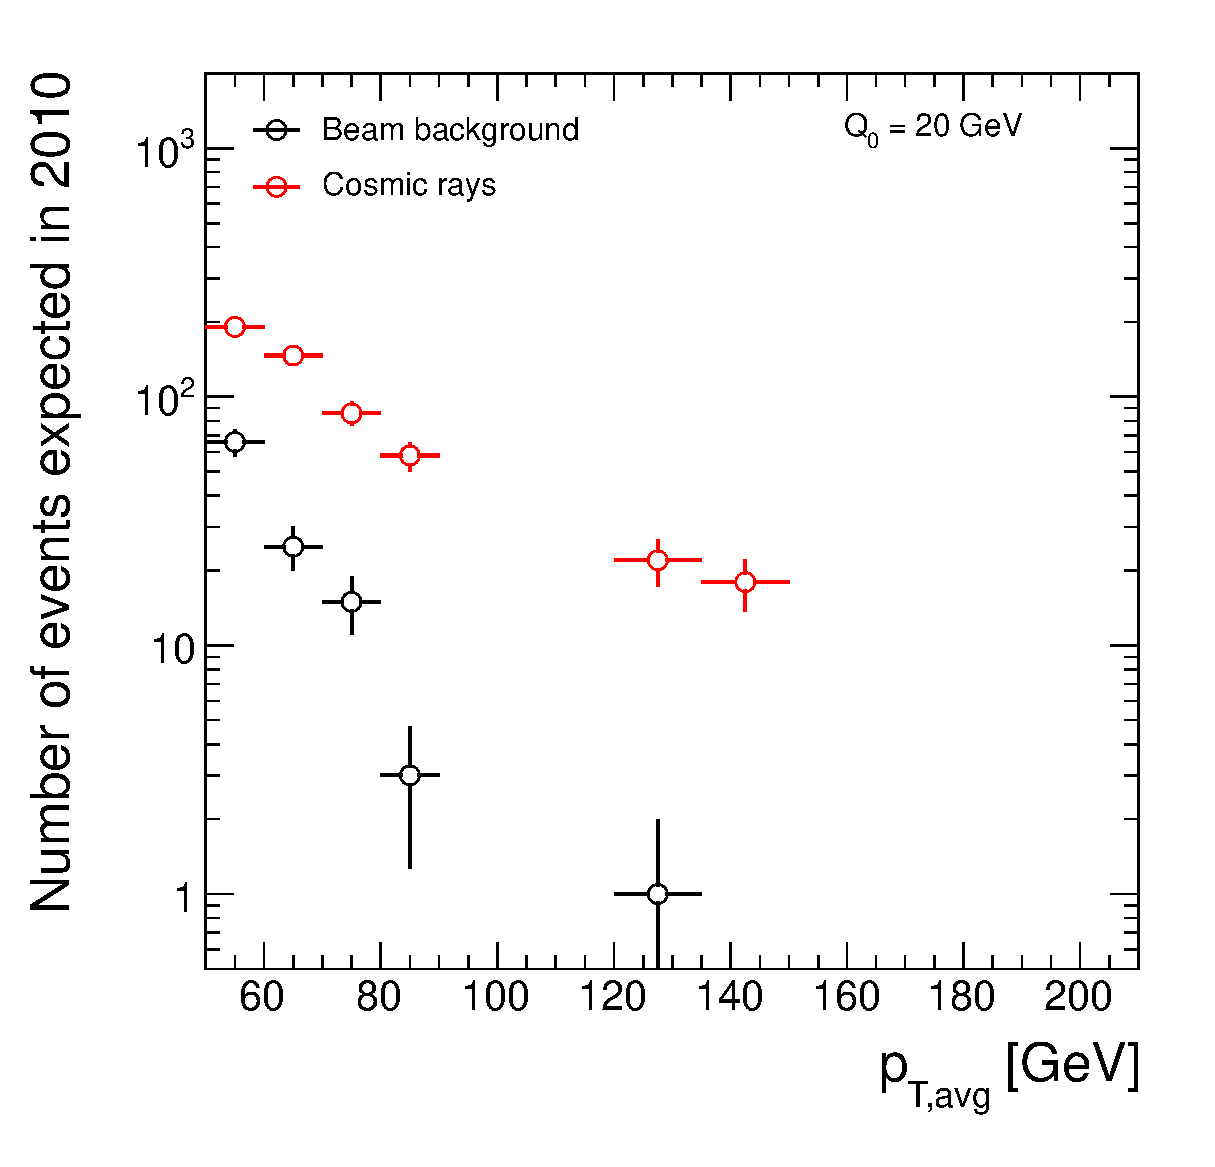
\includegraphics[width=\smallfigwidth]{chapters/gbj/Backgrounds.SelectionA.pTbar.eps}
    \label{fig:gbj:backgrounds}}
  \quad
  \subfloat[Effect of jet cleaning cuts on gap fraction]{
    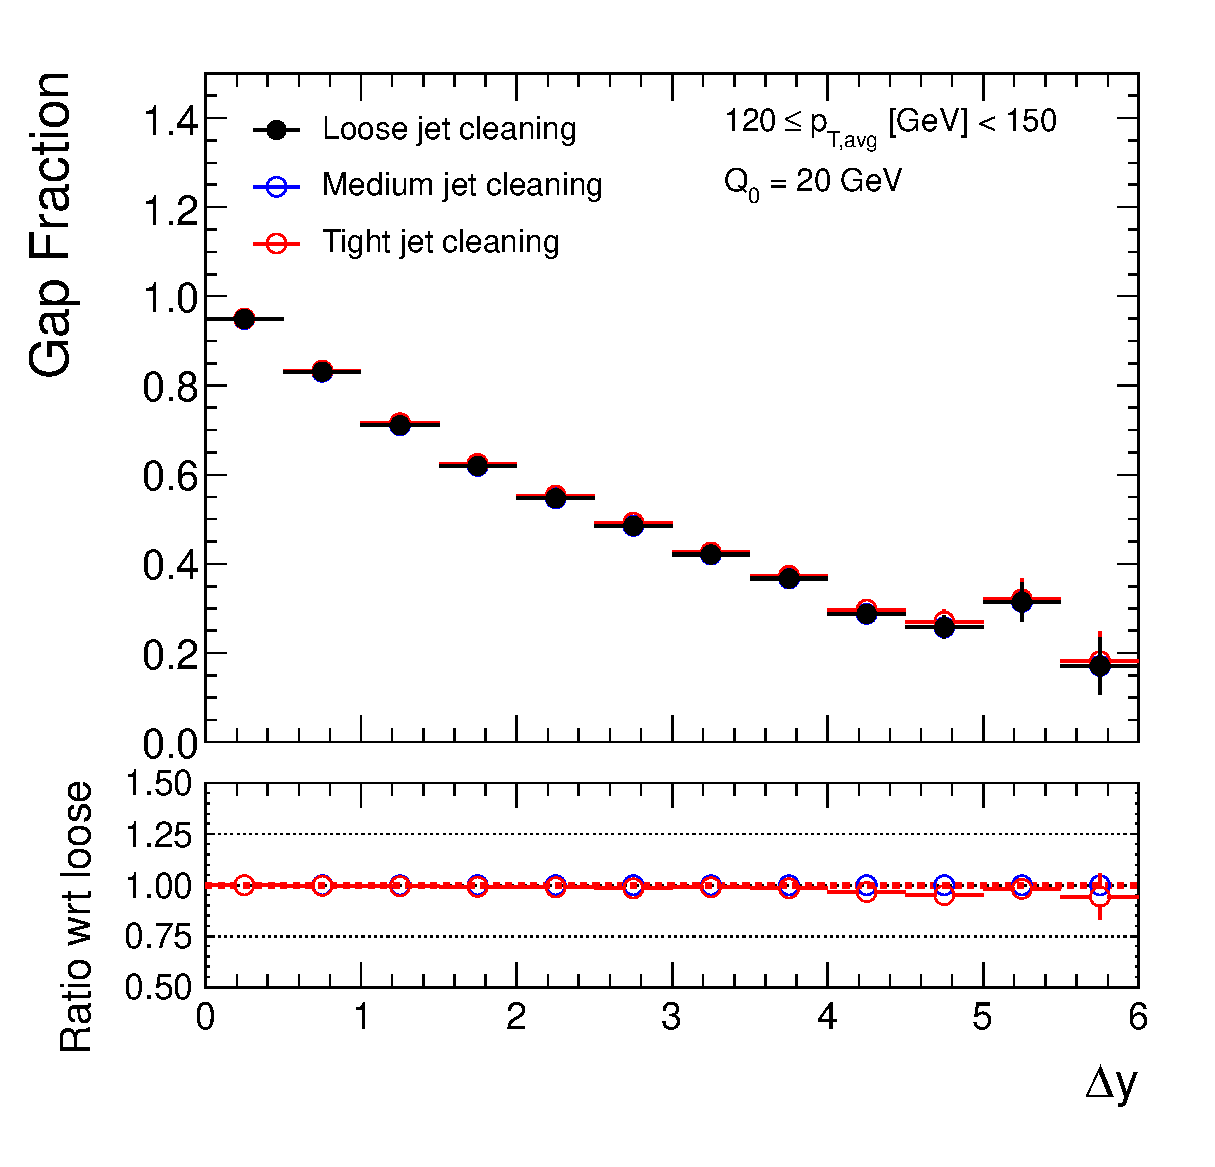
\includegraphics[width=\smallfigwidth]{chapters/gbj/QualityComparison.GapFraction.SelectionA.120pT150.dYBins.eps}
    \label{fig:gbj:quality_comparison}}
  \caption{Control distributions, used to demonstrate the effects of some potential sources of systematic error. \protect\subref{fig:gbj:backgrounds} shows the \DeltaY distribution of events arising from beam background and cosmic rays. The overall number of accepted signal events was approximately $5 \times 10^{5}$ inclusive and $4 \times 10^{5}$ gap events, so these backgrounds represent only a small perturbation and do not need to be explicitly corrected for. \protect\subref{fig:gbj:quality_comparison} shows the effect on the gap fraction as a function of \Qnought of applying different jet cleaning cuts; the differences arising in the final distributions are found to be negligible.}
  \label{fig:gbj:control_distributions}
\end{figure}

The final systematic uncertainty is obtained by summing each of these components in quadrature.
\FigureRef{fig:gbj:systematics_summary} shows an example of how the relative systematic
uncertainty changes with the \DeltaY of the boundary jets, both for the gap fraction
and the mean number of jets in the rapidity interval between the boundary jets.

\begin{figure}[htpb]
  \subfloat[Gap fraction systematics]{
    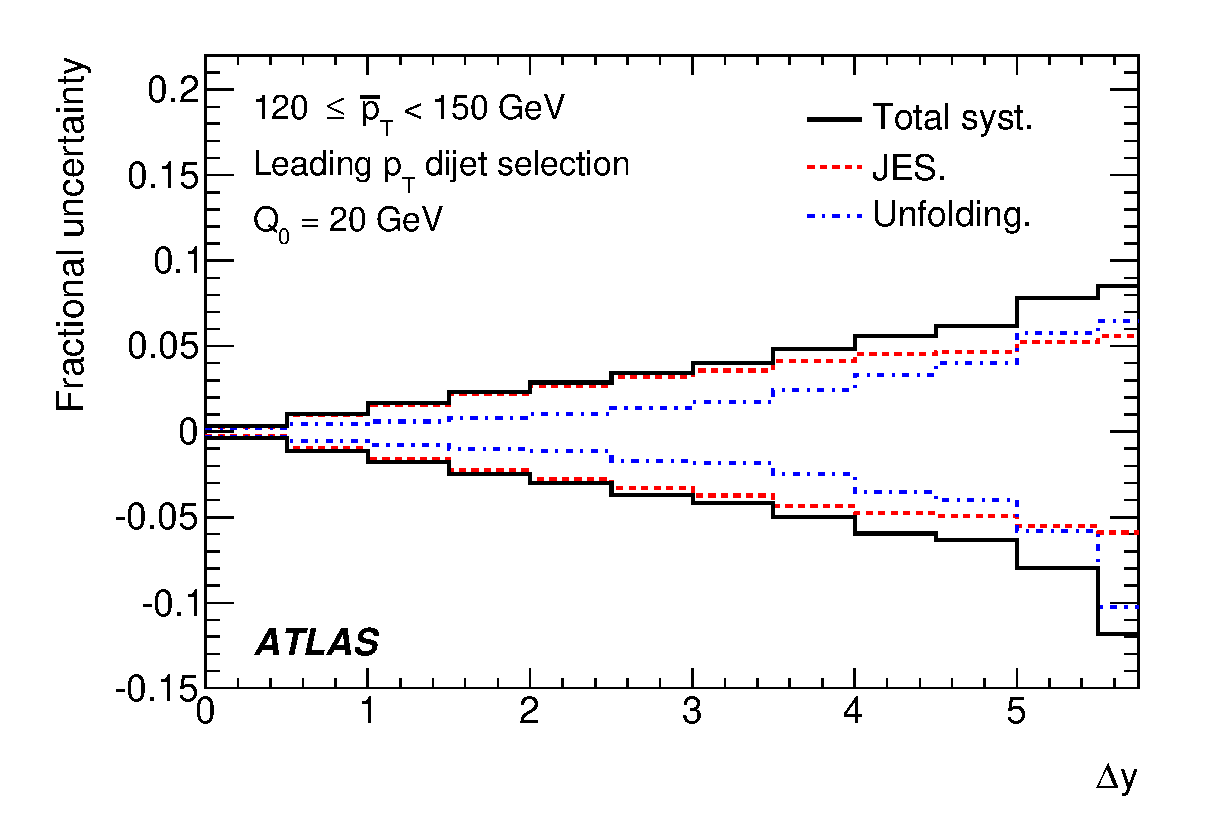
\includegraphics[width=\smallfigwidth]{chapters/gbj/Systematics_GapFraction_YDist_gap_Q0_selA_PtBar_120_150.eps}
    \label{fig:gbj:systematics_gap_fraction}}
  \quad
  \subfloat[\pTbar systematics]{
    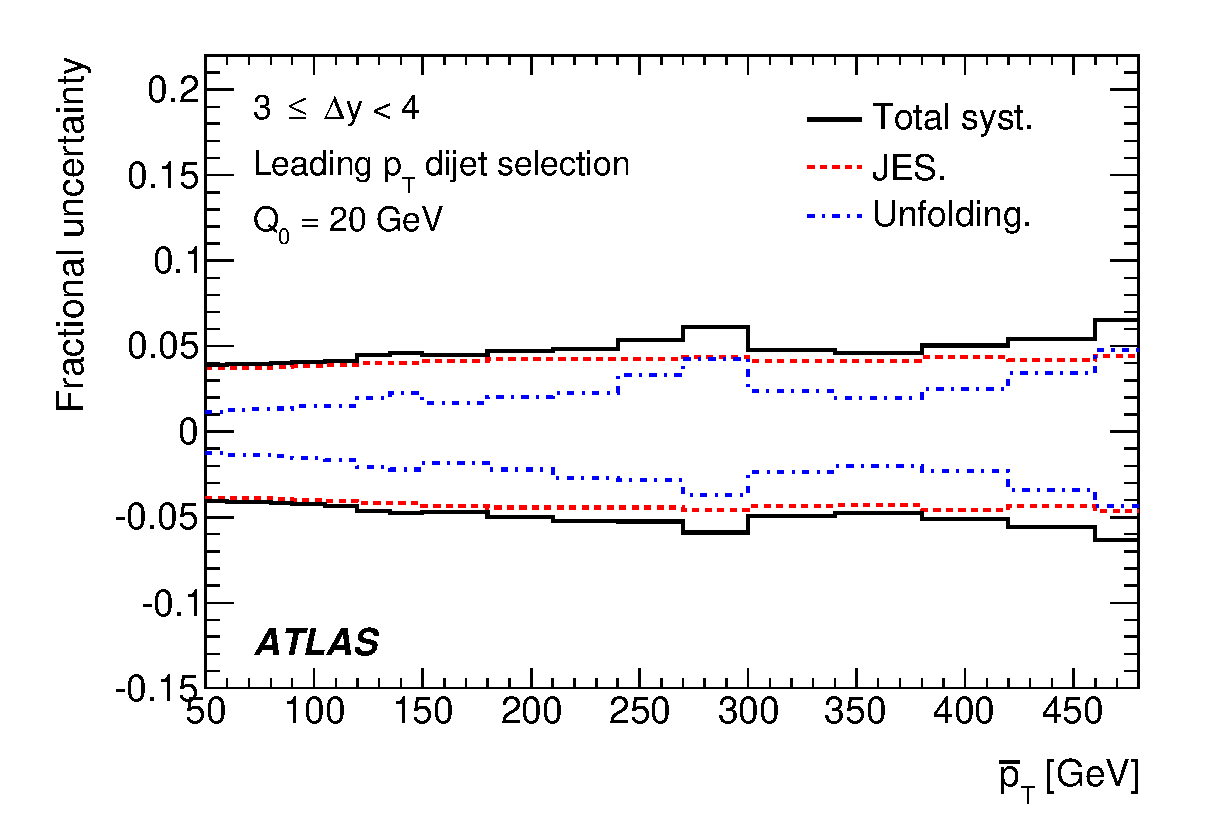
\includegraphics[width=\smallfigwidth]{chapters/gbj/Systematics_GapFraction_PtBarDist_gap_Q0_selA_Y_3_4.eps}
    \label{fig:gbj:systematics_n_jets_avg}}
  \caption{Example of the contributions to the systematic uncertainty for selection A data with $\Qnought = \unit{20}{\GeV}$: \protect\subref{fig:gbj:systematics_gap_fraction} on the gap fraction, for $120 \leq \pTbar < 150 \GeV$, \protect\subref{fig:gbj:systematics_n_jets_avg} on the mean number of jets in the rapidity interval between the boundary jets, for $3 \leq \DeltaY < 4$.}  
  \label{fig:gbj:systematics_summary}
\end{figure}

The irregularity at approximately \unit{290}{\GeV} that can be seen in the uncertainty
arising from the unfolding procedure is caused by the way in which the relevant \MC samples are produced. Samples
are created in bins of \pT, with statistics at the high end of one sample lower
than the statistics available at the low end of the next sample. Such differences
at the boundaries between samples, often cause statistical fluctuations when the
results are combined.

\subsection{Effect of Jet Energy Scale Uncertainty}
\label{sec:gbj:jes_uncertainty}
Jet energy scale (JES) uncertainties are available as a function of jet transverse
momentum and rapidity from a dedicated \ATLAS tool~\cite{ATLAS-CONF-2010-056}.
Both absolute and relative jet energy scale (JES) uncertainty affect this measurement.
The effect of the absolute JES uncertainty can be studied by shifting the energy
of all jets by $\pm 1 \sigma$. The effect of this shift on the gap fraction is
small, ranging from 2\% to 5\% across the \pTbar spectrum and from 0.5\% to 5\%
across the \DeltaY spectrum.

Relative JES uncertainty is the uncertainty in calibration between different
rapidity regions of the detector. The largest effect occurs when there is a decorrelation of the
JES uncertainty between the boundary jets and those jets which lie between them
in rapidity. This occurs because of the way that gap and non-gap events are distinguished
using a third jet veto. To estimate the maximum uncertainty arising from this, it is
assumed that the veto jets are central (see \FigureRef{fig:gbj:veto_jet_eta}) and that the maximum
decorrelation between the boundary jets and the veto jets is therefore 3\% when
the most forward boundary jet is central ($|\pseudorap|<2.8$) and 10\% when the
most forward boundary jet is forward ($|\pseudorap|>2.8$). These numbers come
from the \ATLAS JES uncertainty provider~\cite{ATLAS-CONF-2010-056} and are based, in the forward region,
on the results of the \dijet intercalibration (see \FigureRef{fig:etaint:relative_jet_response_uncertainty}).
It is important to note that the data lies within the spread of \MC predictions in the forward region
and hence that this is a conservative overestimate of the true JES uncertainty.
The uncertainty on the gap fraction deriving from the effects of relative JES uncertainty
is approximately 2\% across the \pTbar distribution and between 0.5\% and 10\% across
the \DeltaY distribution.

\begin{figure}[htpb]
  \subfloat[Veto jet \pseudorap distribution]{
    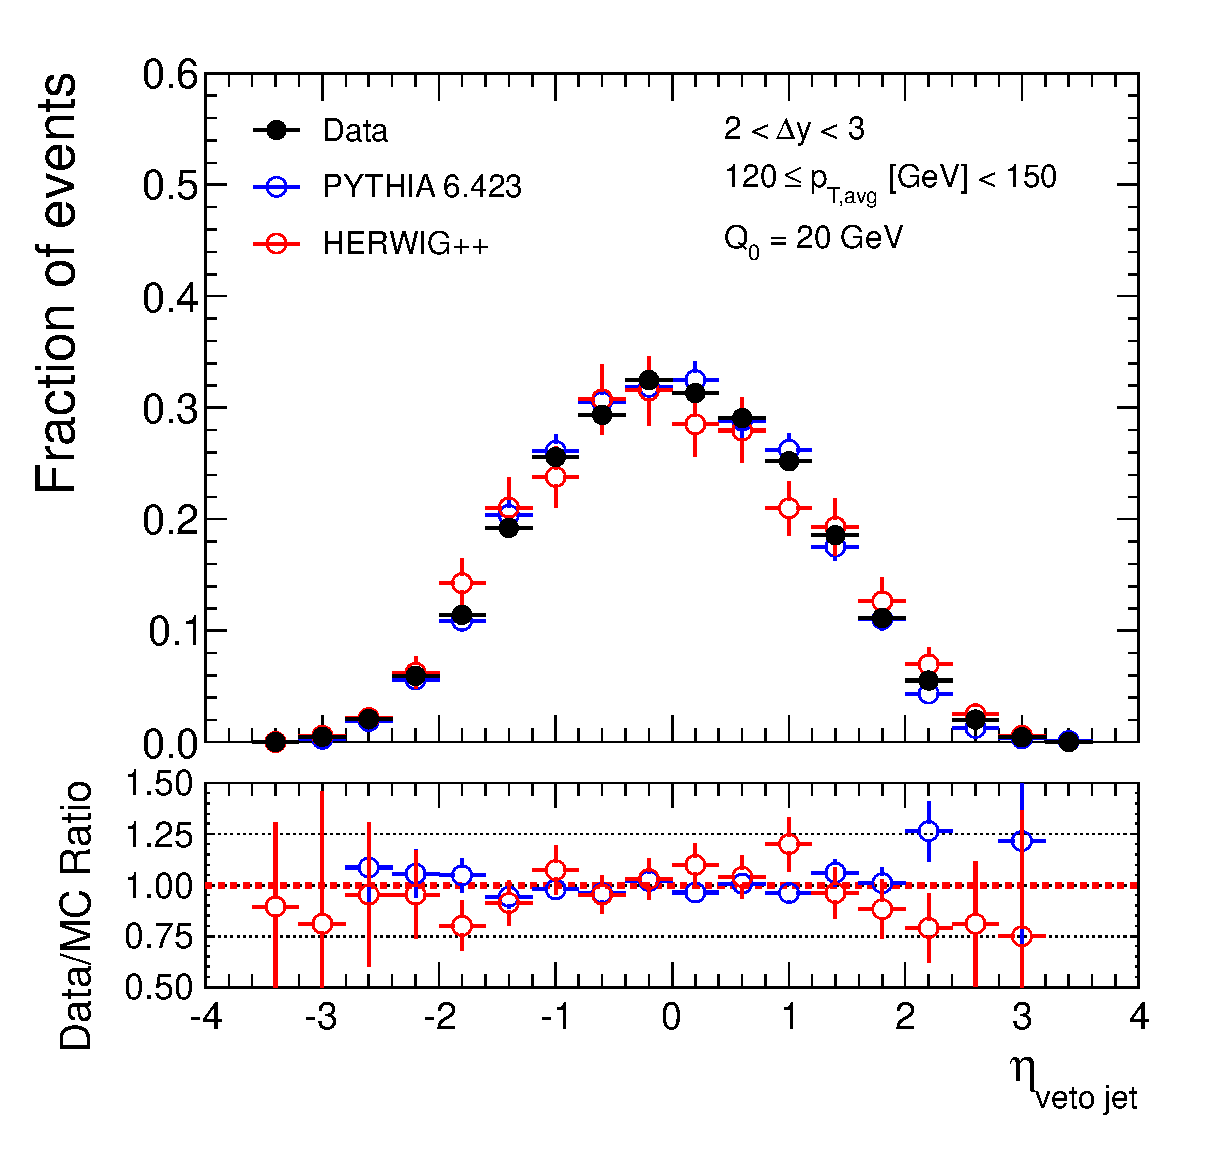
\includegraphics[width=\smallfigwidth]{chapters/gbj/VetoJetEta.SelectionA.Q020.2dY3.120pT150.eps}
    \label{fig:gbj:veto_jet_eta}}
  \quad
  \subfloat[Veto jet \pT distribution]{
    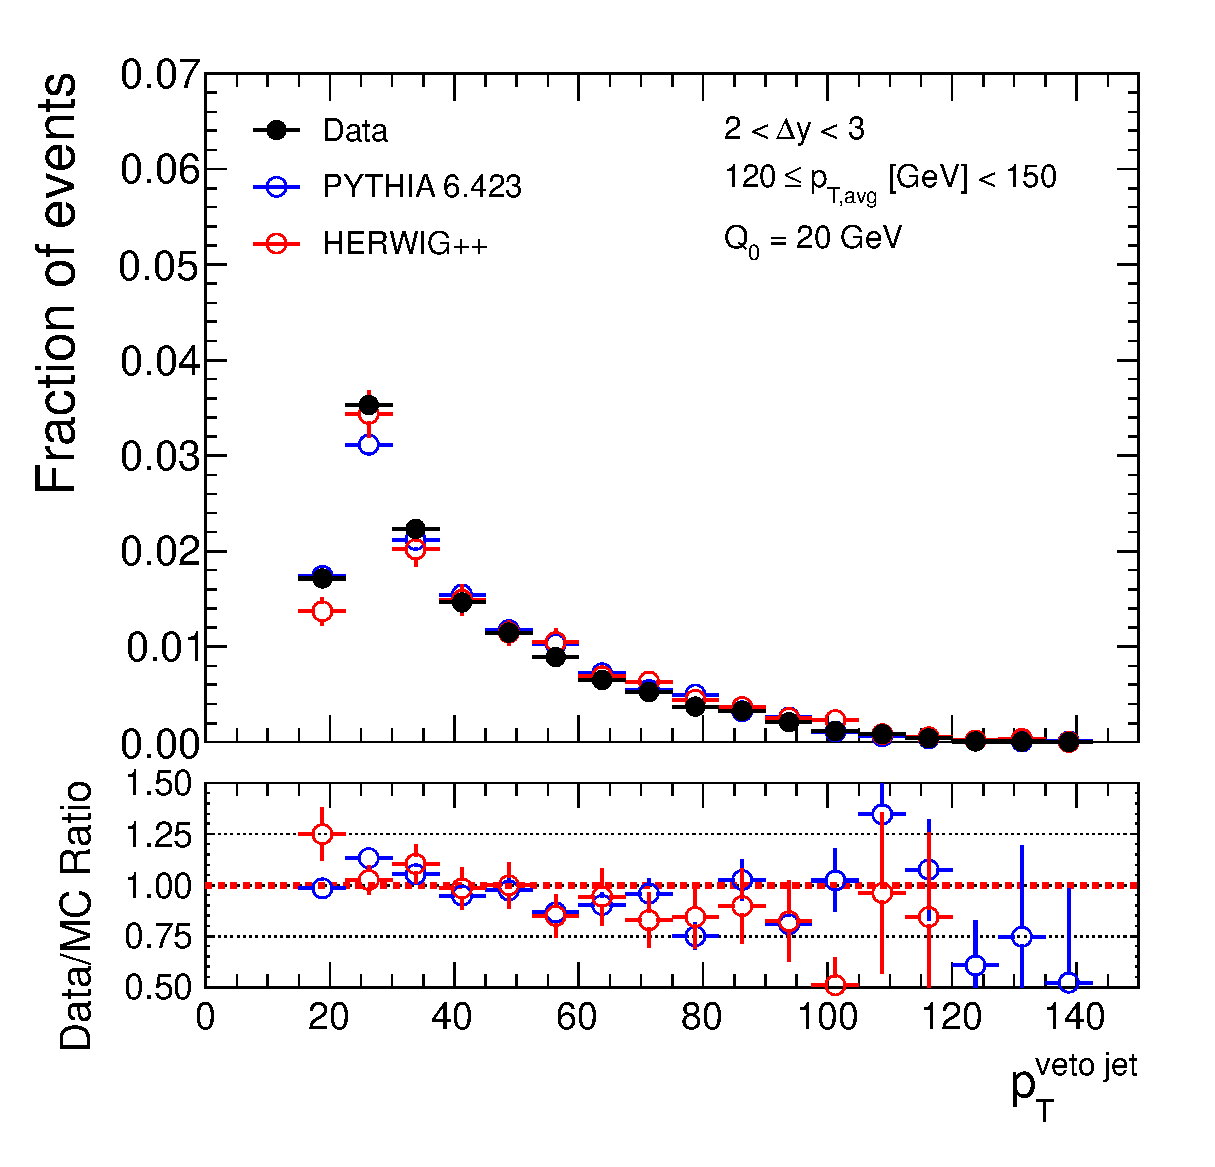
\includegraphics[width=\smallfigwidth]{chapters/gbj/VetoJetPT.SelectionA.Q020.2dY3.120pT150.eps}
    \label{c}}
  \caption{The distributions of jets which are above the veto threshold, $\Qnought = \unit{20}{\GeV}$, and in the rapidity gap between the boundary jets in \protect\subref{fig:gbj:veto_jet_eta} \pseudorap and \protect\subref{fig:gbj:veto_jet_eta} \pT.}
  \label{fig:gbj:veto_jet}
\end{figure}

\subsection{Unfolding Detector Effects and Associated Systematic Uncertainty}
\label{sec:gbj:unfolding}
For this analysis, bin-by-bin unfolding (see \SectionRef{sec:analysis-tools:unfolding})
is used as the level of migration between bins for the gap fraction is small as
a function of both \pTbar and \DeltaY.

The calculation of the unfolding correction factors is performed with \Pythia,
\Herwigpp and \Alpgen (see \SectionRef{sec:bg-theory:MC_generators}). Each of
the resultant correction factors is close to unity, with a typical deviation
being smaller than 0.01; as such, the effect of unfolding is much smaller than
the other systematic uncertainties in the analysis. Because of this, an
unfolding correction is applied; instead a systematic error associated with
unfolding is assigned as the quadrature sum of the following three quantities:
the deviation from unity of the unfolding factor obtained with \Pythia; the
statistical error on the unfolding factor obtained with \Pythia; the difference in unfolding
factors obtained when the shapes of the \pTbar, \DeltaY and \pTthree truth
distributions are changed by the maximal amount which produces detector level
distributions that are still compatible with the observed data.

\FigureRef{fig:gbj:data_mc_control_distributions} shows the level of agreement
between \Pythia and the data for two sample distributions; this provides a cross-check
that using \Pythia for the unfolding does not introduce any strong biases.

\begin{figure}[htpb]
  \subfloat[Selection A. Data to \MC comparison as a function of \pTbar]{
    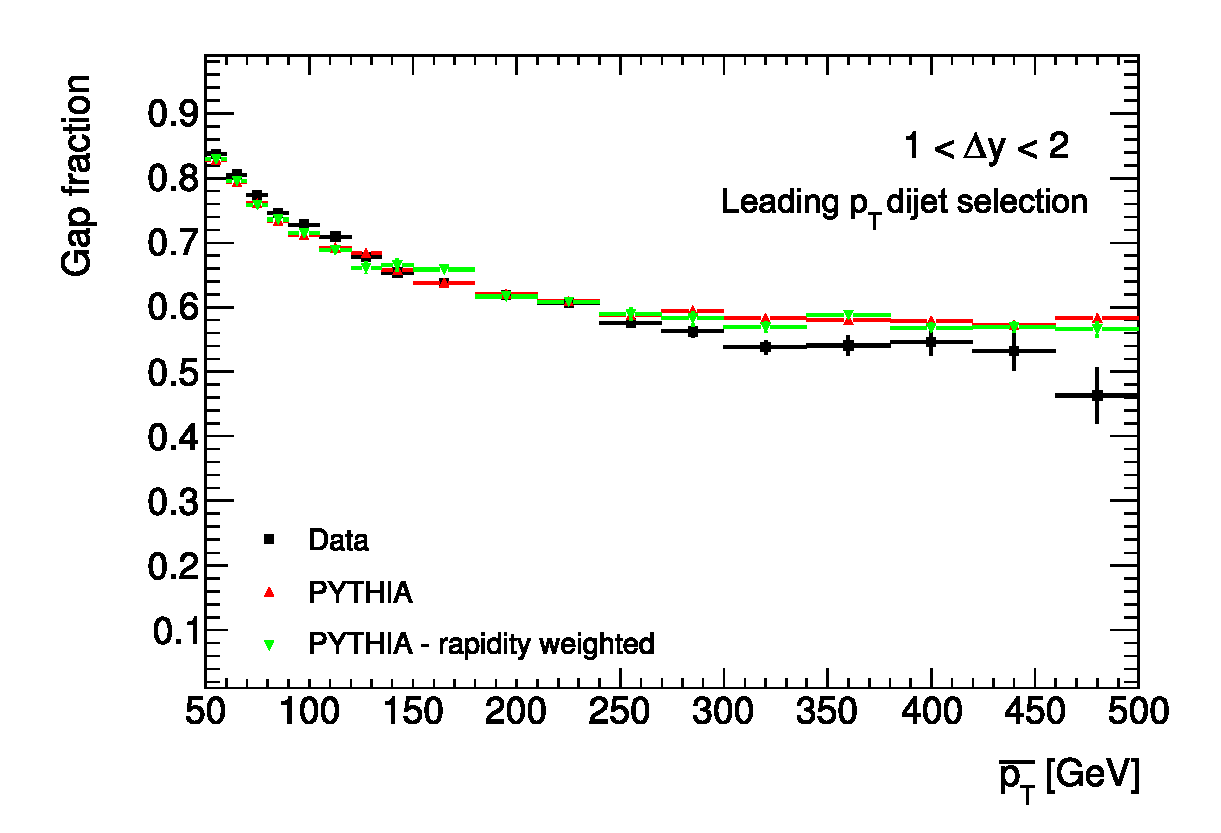
\includegraphics[width=\smallfigwidth]{chapters/gbj/Control.GapFractionPtBardist_1_2_selA_gap_Q0.eps}
    \label{fig:gbj:selectionA_control_dy}}
  \quad
  \subfloat[Selection B. Data to \MC comparison as a function of \DeltaY for inclusive events]{
    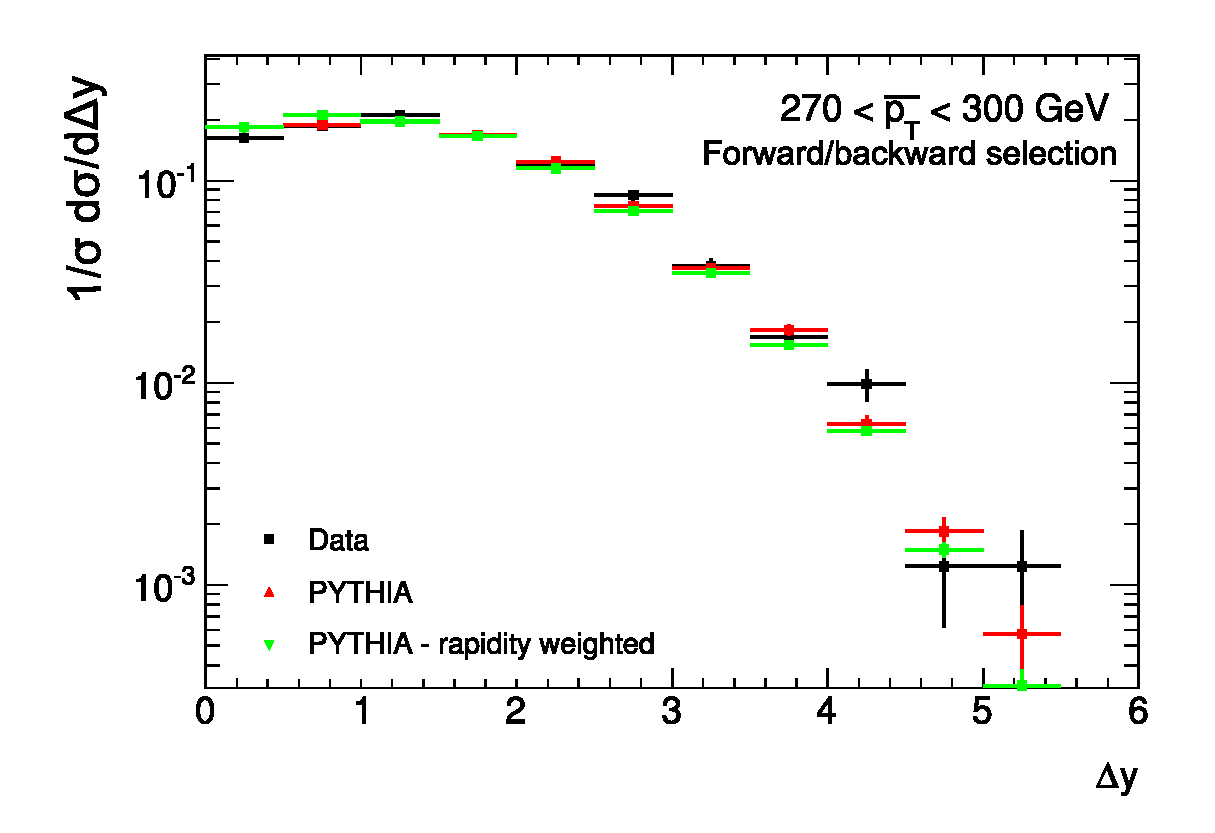
\includegraphics[width=\smallfigwidth]{chapters/gbj/Control.InclusiveJetsYdist_270_300_selB_gap_ptbar.eps}
    \label{fig:gbj:selectionB_control_pTbar}}
  \caption{Control distributions, used to demonstrate the level of agreement between data and \MC. Data is shown in black, with \Pythia in red and specially generated \Pythia samples which are weighted in \rap in green. \protect\subref{fig:gbj:selectionA_control_dy} shows the comparison in the gap fraction as a function of \pTbar for selection A, with $1 \leq \DeltaY < 2$. \protect\subref{fig:gbj:selectionB_control_pTbar} shows the comparison as a function of \DeltaY for inclusive events in selection B, with $270 \leq \pTbar < \unit{300}{\GeV}$.}
  \label{fig:gbj:data_mc_control_distributions}
\end{figure}

The final uncertainty in unfolding is typically much smaller than the JES uncertainty, except
in the largest \pTbar and \DeltaY bins, where the \MC statistics are poor. In these bins,
the unfolding uncertainty can be larger than 5\% (see \FigureRef{fig:gbj:systematics_summary}).
The correction factors predicted independently by \Herwigpp and \Alpgen agree within the statistical uncertainty of each sample.

\section{Theoretical Predictions}
The measurements presented here probe perturbative \QCD in the region where the energy
scale of the \dijet system is larger than the scale of any additional radiation. At large values of
\pTbar/\Qnought or of \DeltaY, it is expected that fixed order calculations are unlikely to describe the data and
that a resummation to all orders in perturbation theory is necessary. These measurements are not
particularly sensitive to non-perturbative physics because \Qnought is chosen to be much greater than
$\Lambda_{QCD}$. The net effect of corrections arising from non-perturbative physics is estimated by turning the
hadronisation and underlying event on and off in \Pythia: the resulting shift in the gap fraction
is less than 2\% and the change in the mean number of jets in the rapidity interval bounded by
the \dijet system is less than 4\%.

Theoretical predictions are produced using the next-to-leading order (NLO) \Powheg generator (see \SectionRef{sec:bg-theory:MC:Powheg})
and \HEJ, a parton level event generator that provides an all-order description of wide-angle emissions
of similar transverse momentum (see \SectionRef{sec:bg-theory:MC:HEJ}). In this \BFKL-inspired limit, \HEJ reproduces the full \QCD results
and should be especially suited for events with at least two jets separated by a large rapidity interval. \HEJ
events are generated with the MSTW 2008 NLO PDF set~\cite{Martin:2009:lhcpartons,Sherstnev:2008:LOMC}
and with the renormalisation and factorisation scales chosen to be the \pT of the leading parton. The uncertainty
due to this scale choice was estimated by increasing and decreasing each scale by a factor of two.
Uncertainties coming from the choice of PDF are estimated using the full set of eigenvector errors provided
by MSTW and also by changing the PDF to CTEQ6L1~\cite{Pumplin:2002:CTEQ6L1}. The overall uncertainty in the \HEJ
calculation is dominated by the scale choice and is typically 5\% for the gap fraction and 8\% for
the mean number of jets in the rapidity interval bounded by the \dijet system. These uncertainties
are larger than the non-perturbative physics corrections which were therefore incorporated
into the systematic uncertainty in quadrature, rather than being applied explicitly.

\section{Jet Veto Results}
The unfolded data, for specific phase space regions, is compared against three
of the leading order \MC event generators that are commonly used for predictive
purposes in \ATLAS, namely \Pythia, \Herwigpp and \Alpgen. \FigureRef{fig:gbj:mc_gap_fraction_dY} shows the gap fraction
as a function of \DeltaY given that the boundary jets satisfy $90 \leq \pTbar < \unit{120}{\GeV}$.

\begin{figure}[htpb]
  \subfloat[Selection A. Leading \pT \dijet{s}]{
    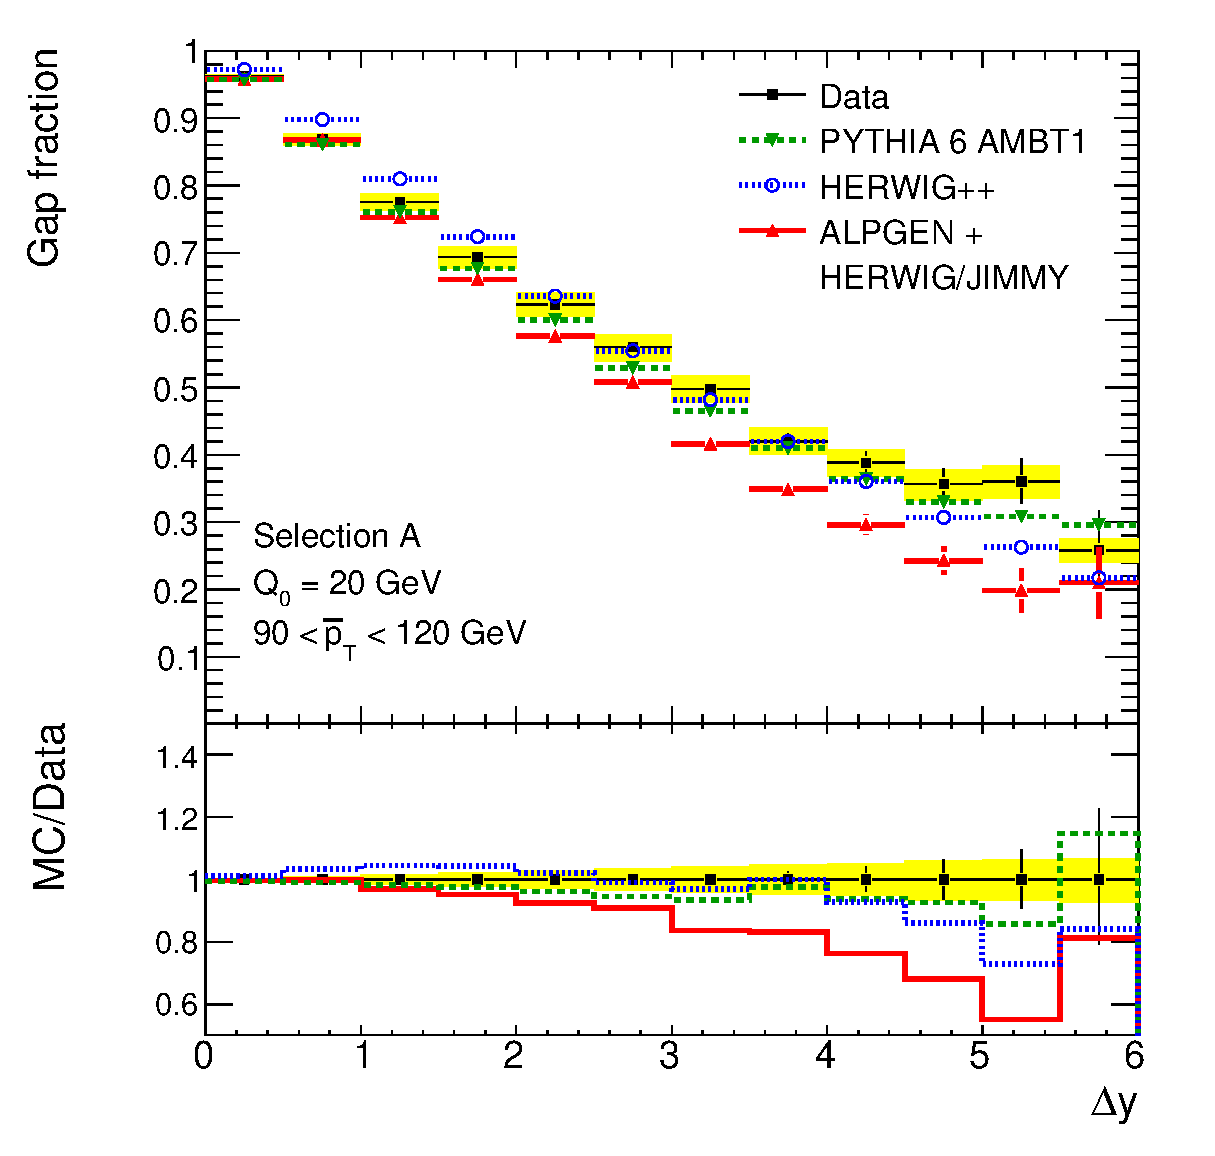
\includegraphics[width=\smallfigwidth]{chapters/gbj/GapFraction_Ydist_MC_selA.eps}
    \label{fig:gbj:mc_gap_fraction_dY_A}}
  \quad
  \subfloat[Selection B. Forward/backward \dijet{s}]{
    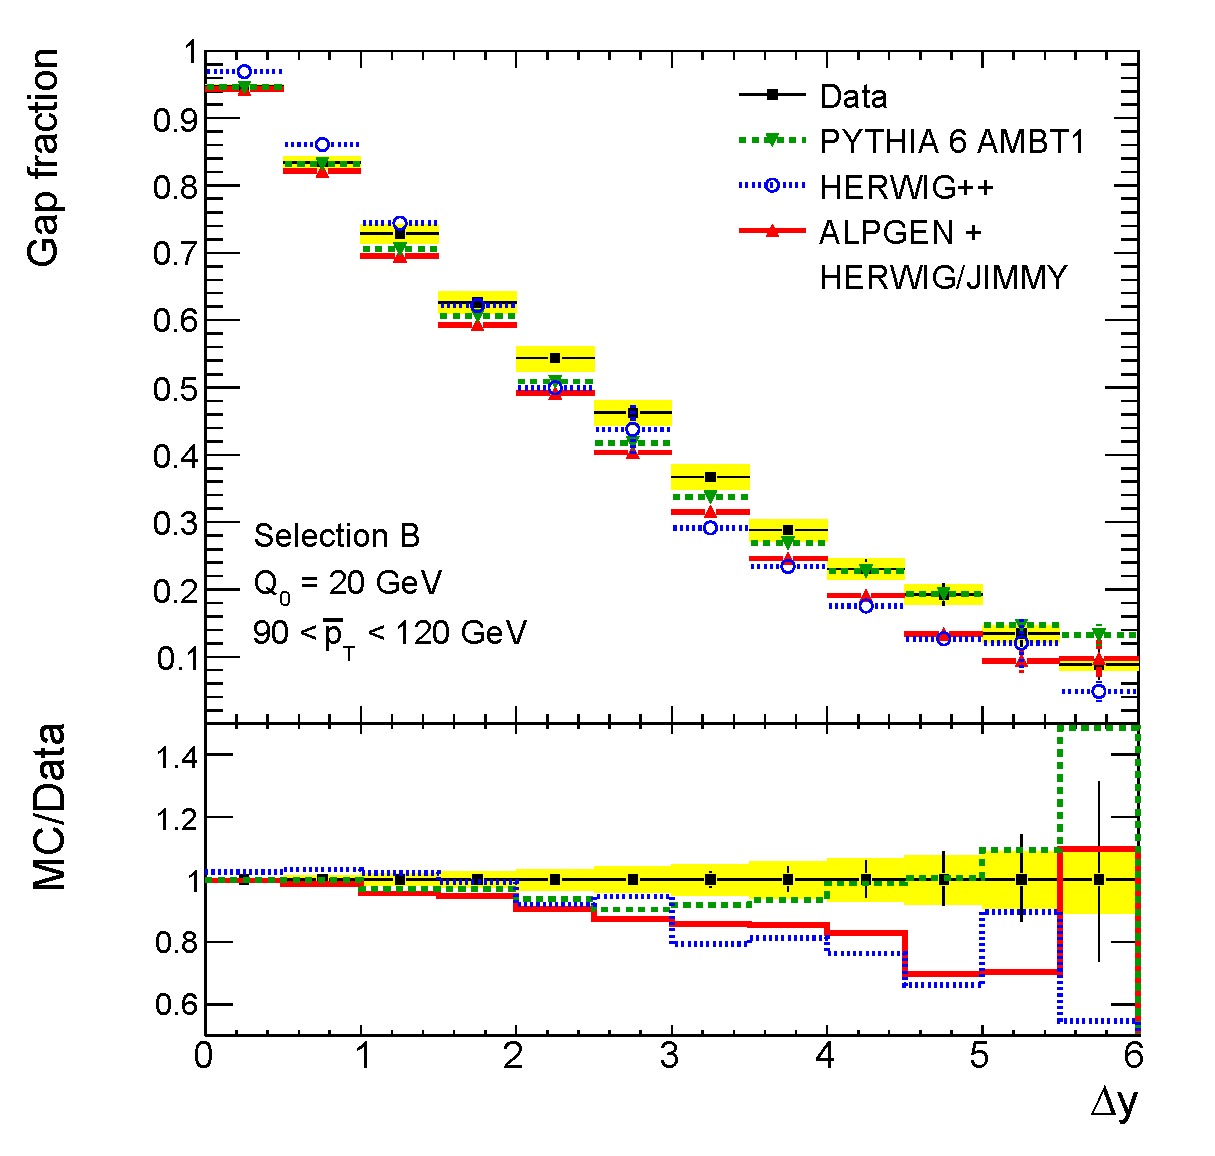
\includegraphics[width=\smallfigwidth]{chapters/gbj/GapFraction_Ydist_MC_selB.eps}
    \label{fig:gbj:mc_gap_fraction_dY_B}}
  \caption{Gap fraction as a function of \DeltaY for boundary jets that satisfy
           $90 \leq \pTbar < \unit{120}{\GeV}$ for \protect\subref{fig:gbj:mc_gap_fraction_dY_A}
           selection A and \protect\subref{fig:gbj:mc_gap_fraction_dY_B} selection B. The (unfolded)
           data are the black points, with error bars representing the statistical
           uncertainty. The systematic uncertainty on the measurement is represented
           by the yellow band. The green curve represents the \Pythia prediction
           (tune AMBT1), the blue curve represents the \Herwigpp prediction (tune
           for LO* PDFs) and the red curve represents the \Alpgen+\Herwig/\Jimmy
           prediction (tune AUET1).}
  \label{fig:gbj:mc_gap_fraction_dY}
\end{figure}

\begin{figure}[htpb]
  \subfloat[Selection A. Leading \pT \dijet{s}]{
    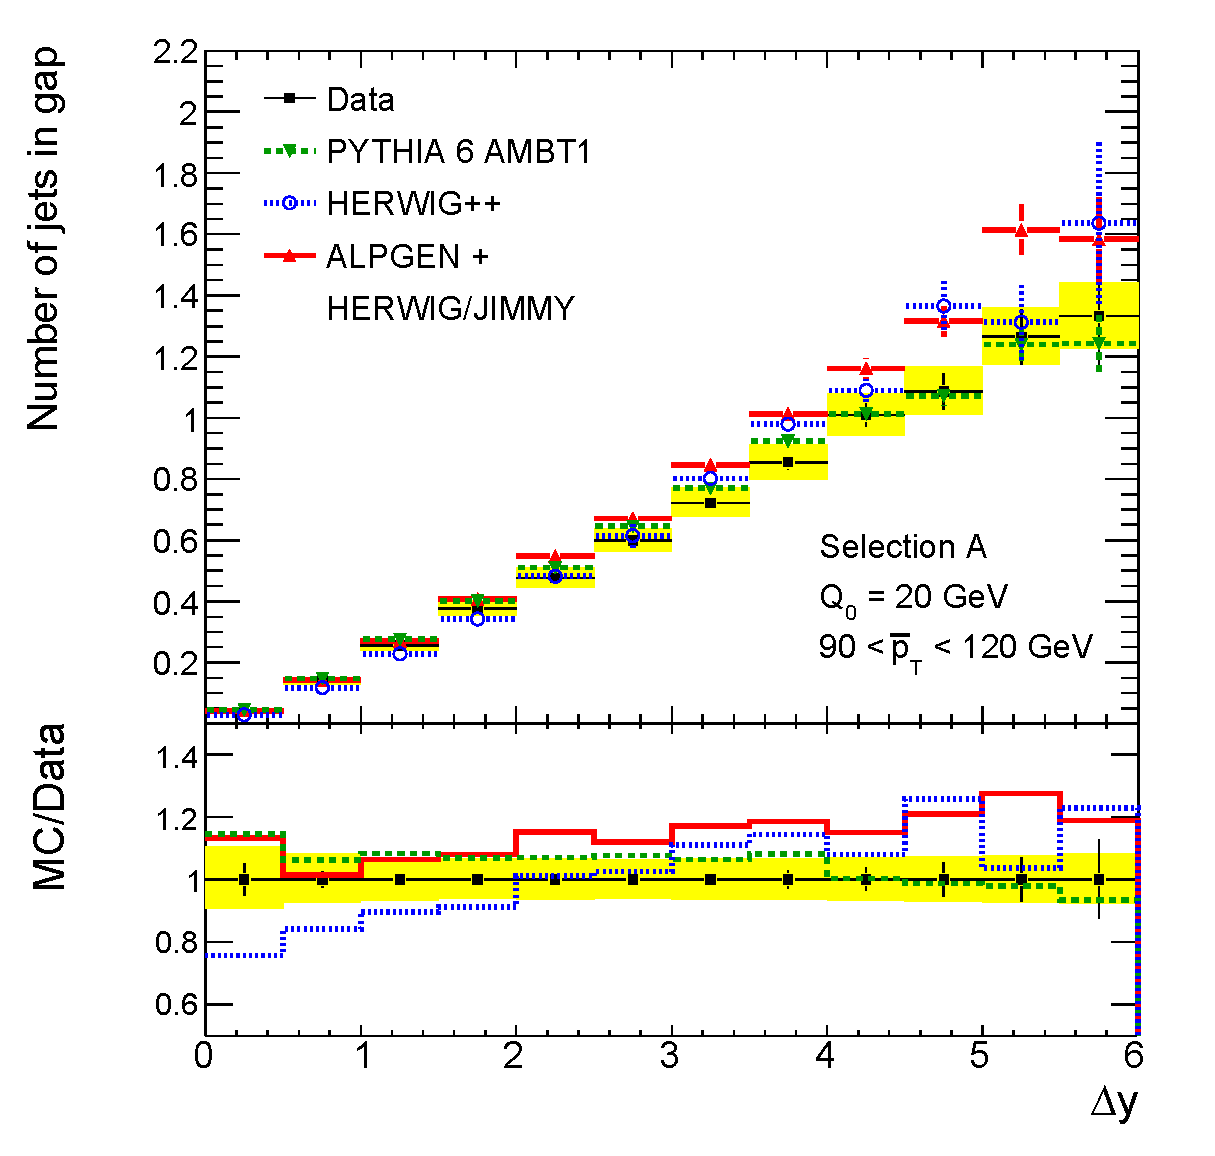
\includegraphics[width=\smallfigwidth]{chapters/gbj/Njet_Ydist_MC_selA.eps}
    \label{fig:gbj:mc_n_jets_dY_A}}
  \quad
  \subfloat[Selection B. Forward/backward \dijet{s}]{
    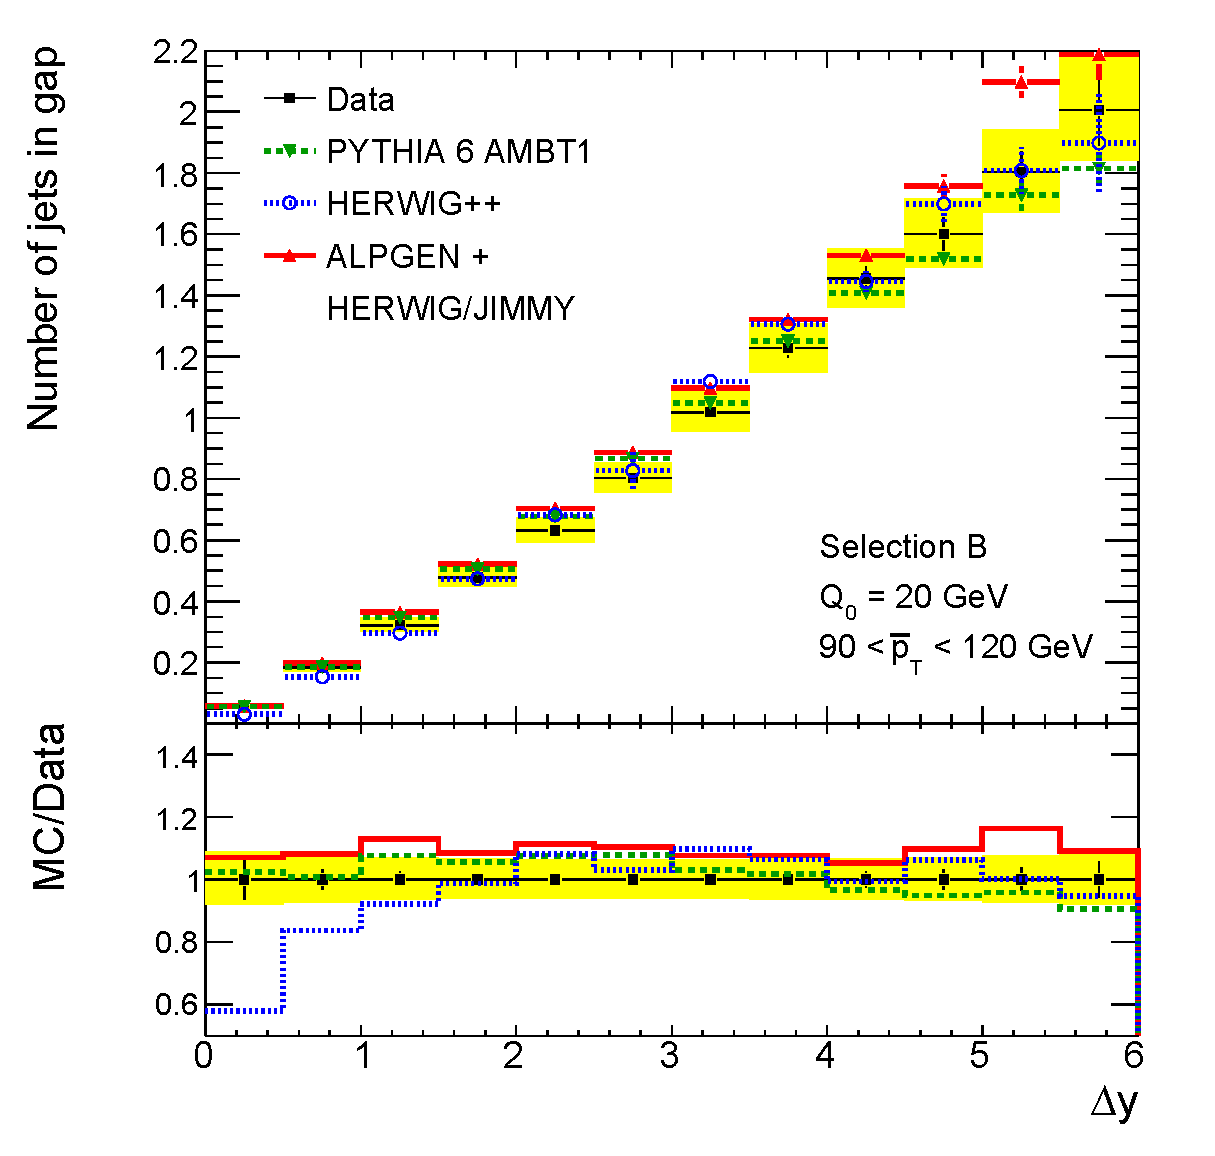
\includegraphics[width=\smallfigwidth]{chapters/gbj/Njet_Ydist_MC_selB.eps}
    \label{fig:gbj:mc_n_jets_dY_B}}
  \caption{Mean number of jets in the rapidity interval between the boundary jets
           as a function of \DeltaY, for boundary jets that satisfy $90 \leq \pTbar < \unit{120}{\GeV}$,
           for \protect\subref{fig:gbj:mc_n_jets_dY_A} selection A and \protect\subref{fig:gbj:mc_n_jets_dY_B}
           selection B. The unfolded data are compared to predictions from three leading-order \MC generators. The data and theory
           are presented in the same way as in \FigureRef{fig:gbj:mc_gap_fraction_dY}.}
           \label{fig:gbj:mc_n_dy}
  \label{fig:gbj:mc_n_jets_dY}
\end{figure}

\begin{figure}[htpb]
  \subfloat[Selection A. Leading \pT \dijet{s}]{
    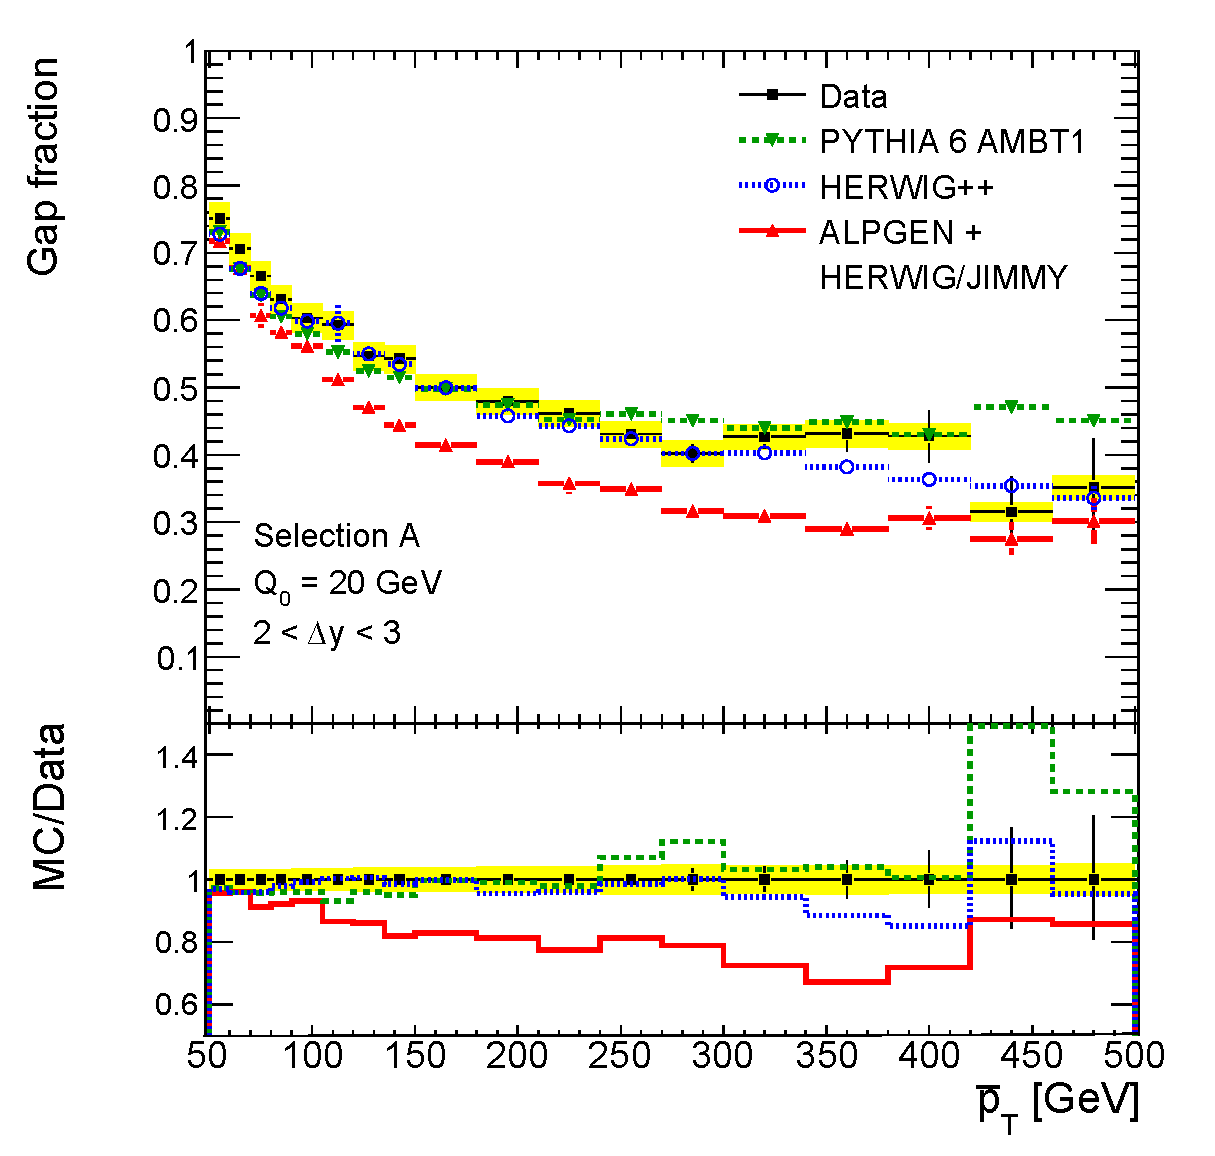
\includegraphics[width=\smallfigwidth]{chapters/gbj/GapFraction_PtBardist_MC_selA.eps}
    \label{fig:gbj:mc_gap_fraction_pTbar_A}}
  \quad
  \subfloat[Selection B. Forward/backward \dijet{s}]{
    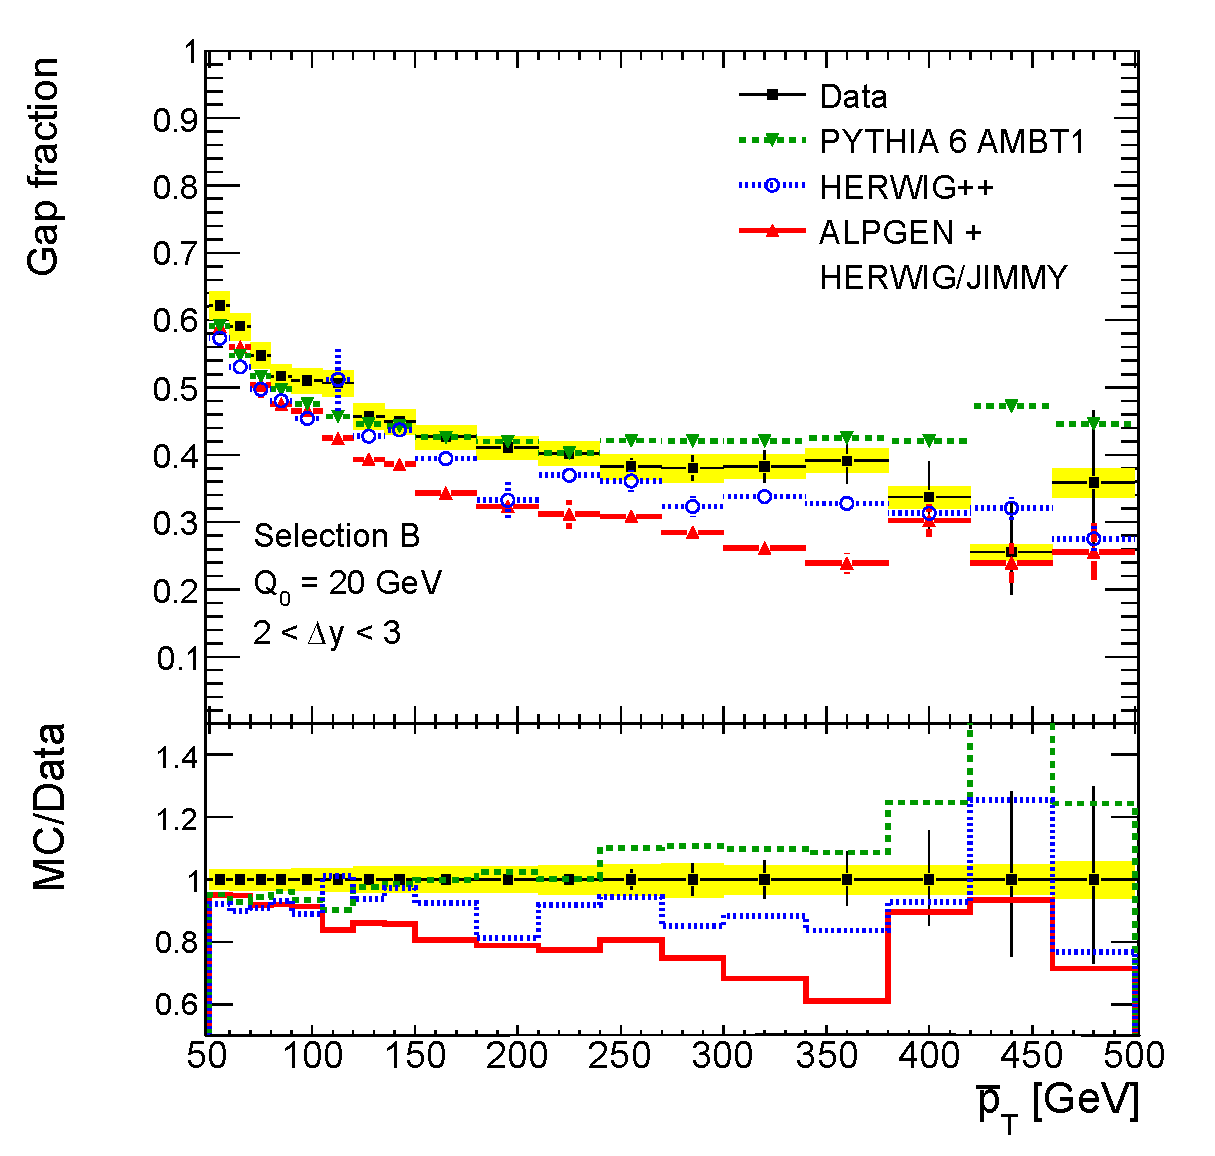
\includegraphics[width=\smallfigwidth]{chapters/gbj/GapFraction_PtBardist_MC_selB.eps}
    \label{fig:gbj:mc_gap_fraction_pTbar_B}}
  \caption{Gap fraction as a function of \pTbar for boundary jets that satisfy $2 \leq \DeltaY < 3$
           for \protect\subref{fig:gbj:mc_gap_fraction_pTbar_A} selection A and \protect\subref{fig:gbj:mc_gap_fraction_pTbar_B}
           selection B. The unfolded data are compared
           to predictions from three leading-order \MC generators. The data and theory
           are presented in the same way as in \FigureRef{fig:gbj:mc_gap_fraction_dY}.}
  \label{fig:gbj:mc_gap_fraction_pTbar}
\end{figure}

\begin{figure}[htpb]
  \subfloat[Selection A. Leading \pT \dijet{s}]{
    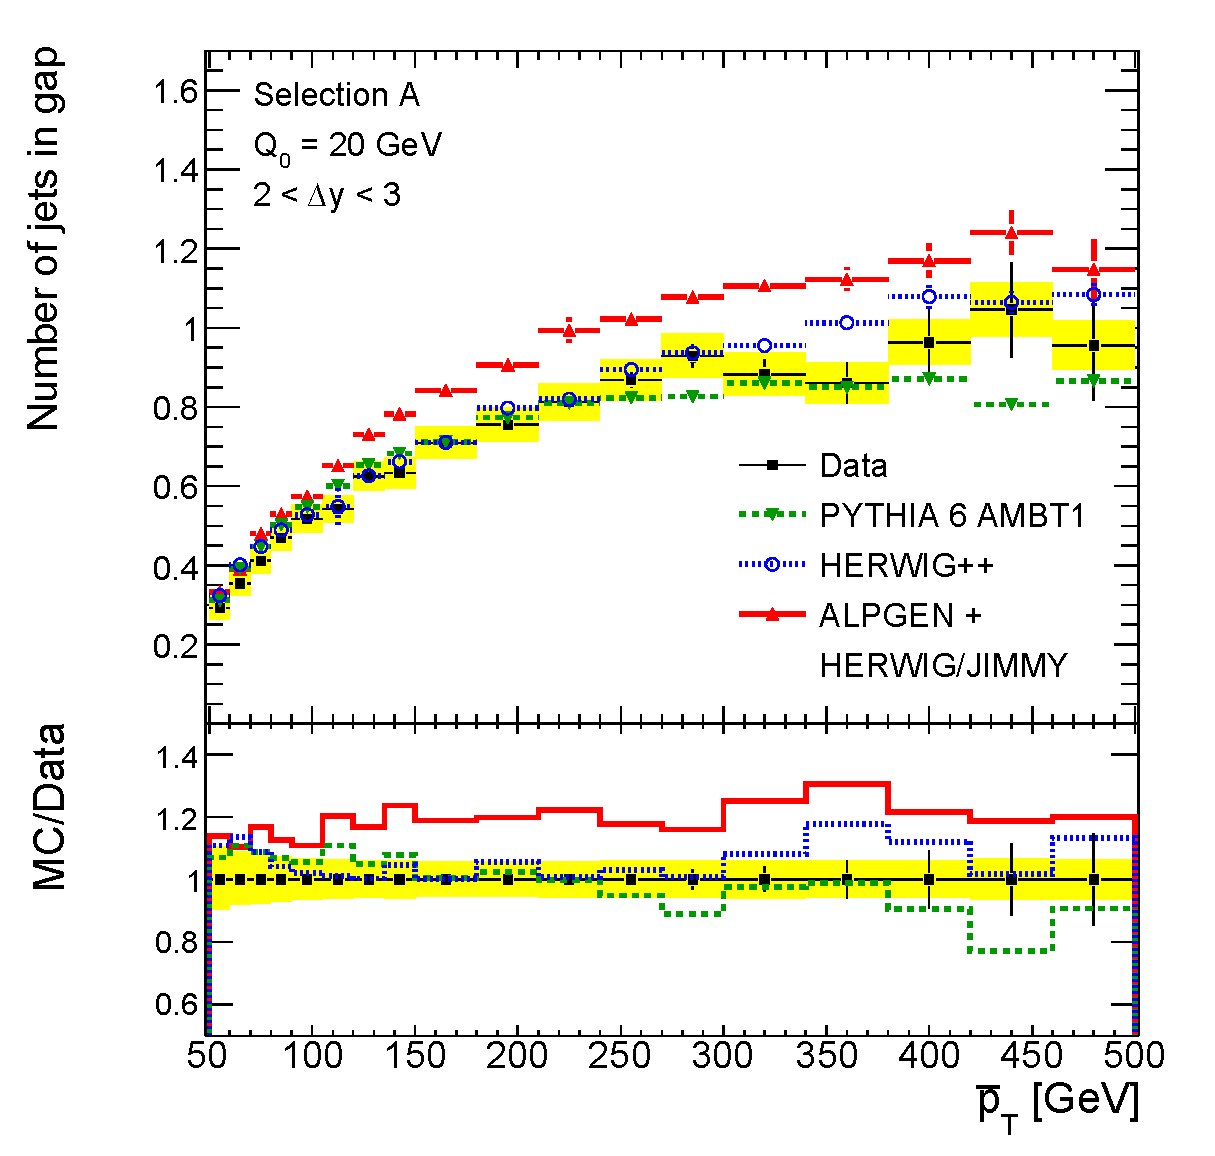
\includegraphics[width=\smallfigwidth]{chapters/gbj/Njet_PtBardist_MC_selA.eps}
    \label{fig:gbj:mc_n_jets_pTbar_A}}
  \quad
  \subfloat[Selection B. Forward/backward \dijet{s}]{
    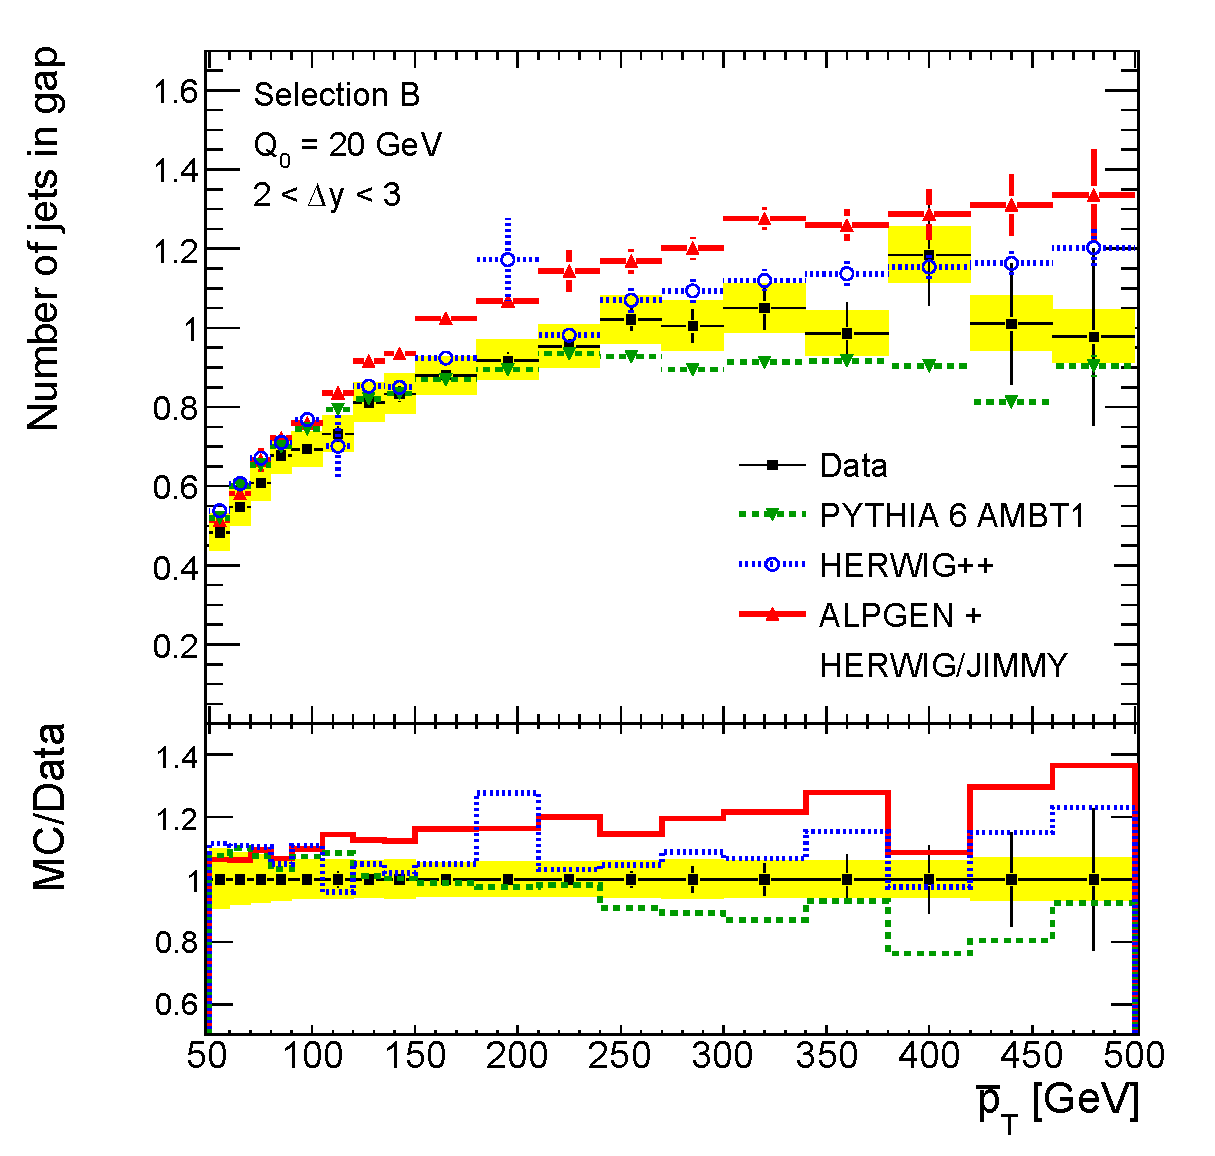
\includegraphics[width=\smallfigwidth]{chapters/gbj/Njet_PtBardist_MC_selB.eps}
    \label{fig:gbj:mc_n_jets_pTbar_B}}
  \caption{Mean number of jets in the rapidity interval between the boundary jets
           as a function of \pTbar, for boundary jets that satisfy $2 \leq \DeltaY < 3$,
           for \protect\subref{fig:gbj:mc_n_jets_pTbar_A} selection A and \protect\subref{fig:gbj:mc_n_jets_pTbar_B}
           selection B. The unfolded data are compared
           to predictions from three leading-order \MC generators. The data and theory
           are presented in the same way as in \FigureRef{fig:gbj:mc_gap_fraction_dY}.}
  \label{fig:gbj:mc_n_jets_pTbar}
\end{figure}

\FigureRef{fig:gbj:mc_n_jets_dY} shows the mean number of jets in the rapidity interval between the boundary jets for
the same cuts. \FigureRef{fig:gbj:mc_gap_fraction_pTbar} shows the gap fraction as a
function of \pTbar given that $2 < \DeltaY < 3$ while \FigureRef{fig:gbj:mc_n_jets_pTbar} shows
the mean number of jets in the rapidity interval between the boundary jets as a function
of \pTbar for the same phase space region.

In all cases, the \MC event generators provide different predictions.
\Pythia tends to slightly overestimate jet activity, and hence underestimate the
gap fraction at low \DeltaY and low \pTbar, but in general gives the best
description of the data. \Herwigpp predicts the gap fraction reasonably well at
low values of \DeltaY, but not the number of jets in the same region, and predicts
too much jet activity, and so too small a gap fraction, at large values of \DeltaY.
\Alpgen shows the largest deviation from the data, predicting too much jet activity, and
thus too low a gap fraction, at large values of \DeltaY and \pTbar. Some of this deviation
can be attributed to the use of \Herwig and \Jimmy for parton shower, hadronisation
and underlying event - \Herwig and \Jimmy implement similar algorithms to those in
\Herwigpp, which also predicts more jet activity than is observed in the data.

The unfolded data, for all phase space regions, is compared to the theoretical
predictions supplied by \Powheg and \HEJ. The \HEJ predictions are presented as a band
in order to represent the theoretical uncertainty due to scale and PDF choices. The \Powheg predictions are presented
after parton showering, hadronisation and underlying event simulation with either \Pythia or \Herwig.
The difference between these two predictions is much larger than the uncertainty
obtained by varying the PDFs or the renormalisation and factorisation scales and
both curves are therefore shown as a conservative estimate of the uncertainty
due to higher order effects. The experimental uncertainties
are much smaller than the theoretical uncertainty on the \HEJ prediction except when
both \DeltaY and \pTbar are large. 

\begin{figure}[htpb]
  \subfloat[\DeltaY slices]{
    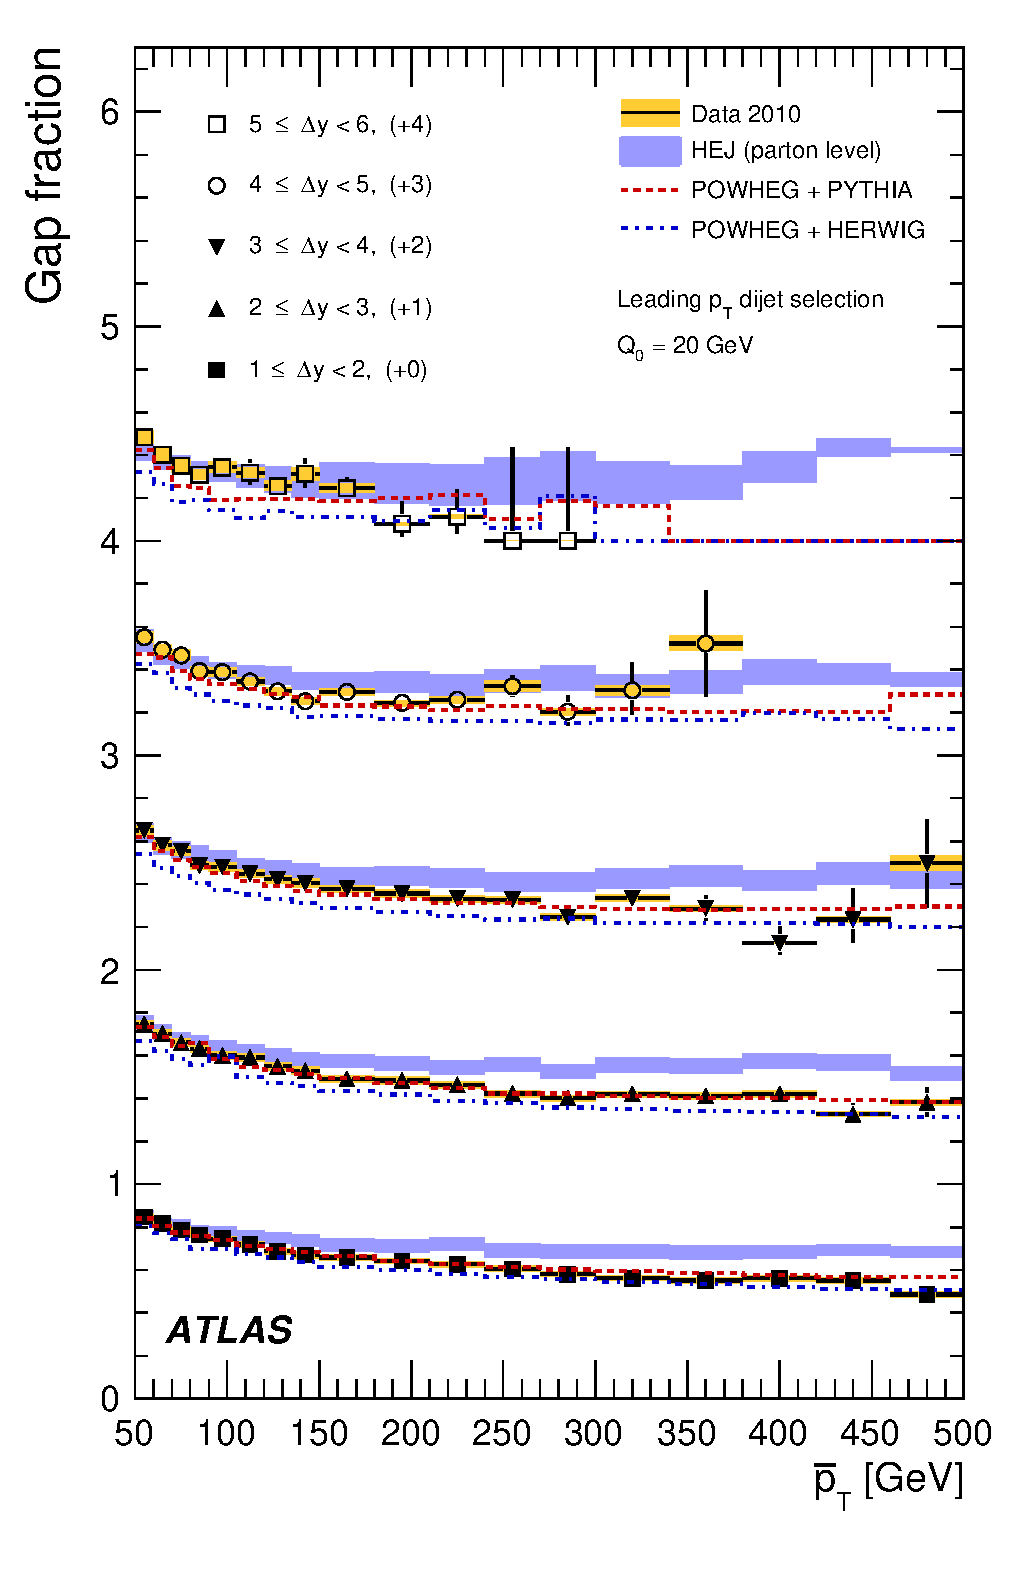
\includegraphics[width=\smallfigwidth]{chapters/gbj/GapFraction_PtBarDist_gap_Q0_sel_A.eps}
    \label{fig:gbj:Gap_fraction_pTbar_A_comparison}}
  \quad
  \subfloat[Ratio to theory]{
    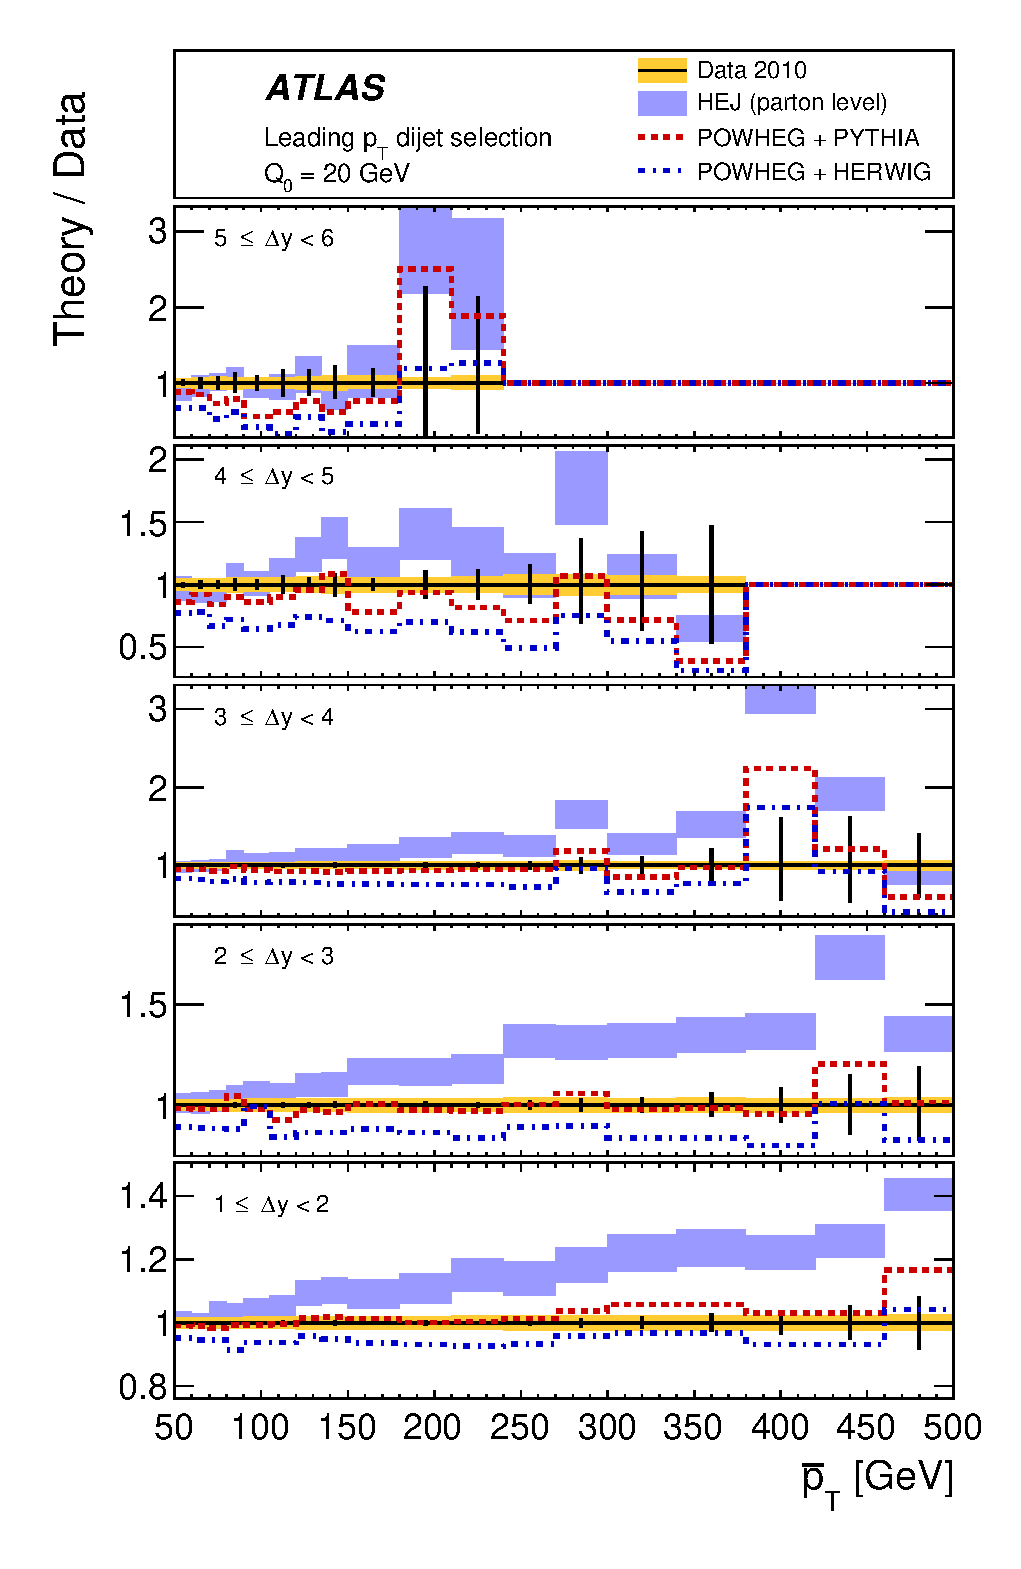
\includegraphics[width=\smallfigwidth]{chapters/gbj/GapFraction_PtBarDist_gap_Q0_sel_A_Ratio.eps}
    \label{fig:gbj:Gap_fraction_pTbar_A_ratio}}
  \caption{Gap fraction as a function of \pTbar for five \DeltaY slices. \protect\subref{fig:gbj:Gap_fraction_pTbar_A_comparison}
           shows selection A data against the \HEJ and \Powheg generators, while \protect\subref{fig:gbj:Gap_fraction_pTbar_A_ratio}
           shows the ratio of the theory predictions to the data. The unfolded data
           are the black points, with error bars representing the statistical uncertainty.
           The systematic uncertainty on the measurement is represented by the yellow band. 
           The light, solid band represents the theoretical uncertainty in the \HEJ calculation
           from variation of the PDF and renormalisation/factorisation scales. The red
           and blue dotted lines represent the \Powheg predictions after showering, hadronisation
           and underlying event simulation with \Pythia (tune AMBT1) and \Herwig+\Jimmy
           (tune AUET1), respectively.}
  \label{fig:gbj:Gap_fraction_pTbar_A}
\end{figure}

\begin{figure}[htpb]
  \subfloat[\DeltaY slices]{
    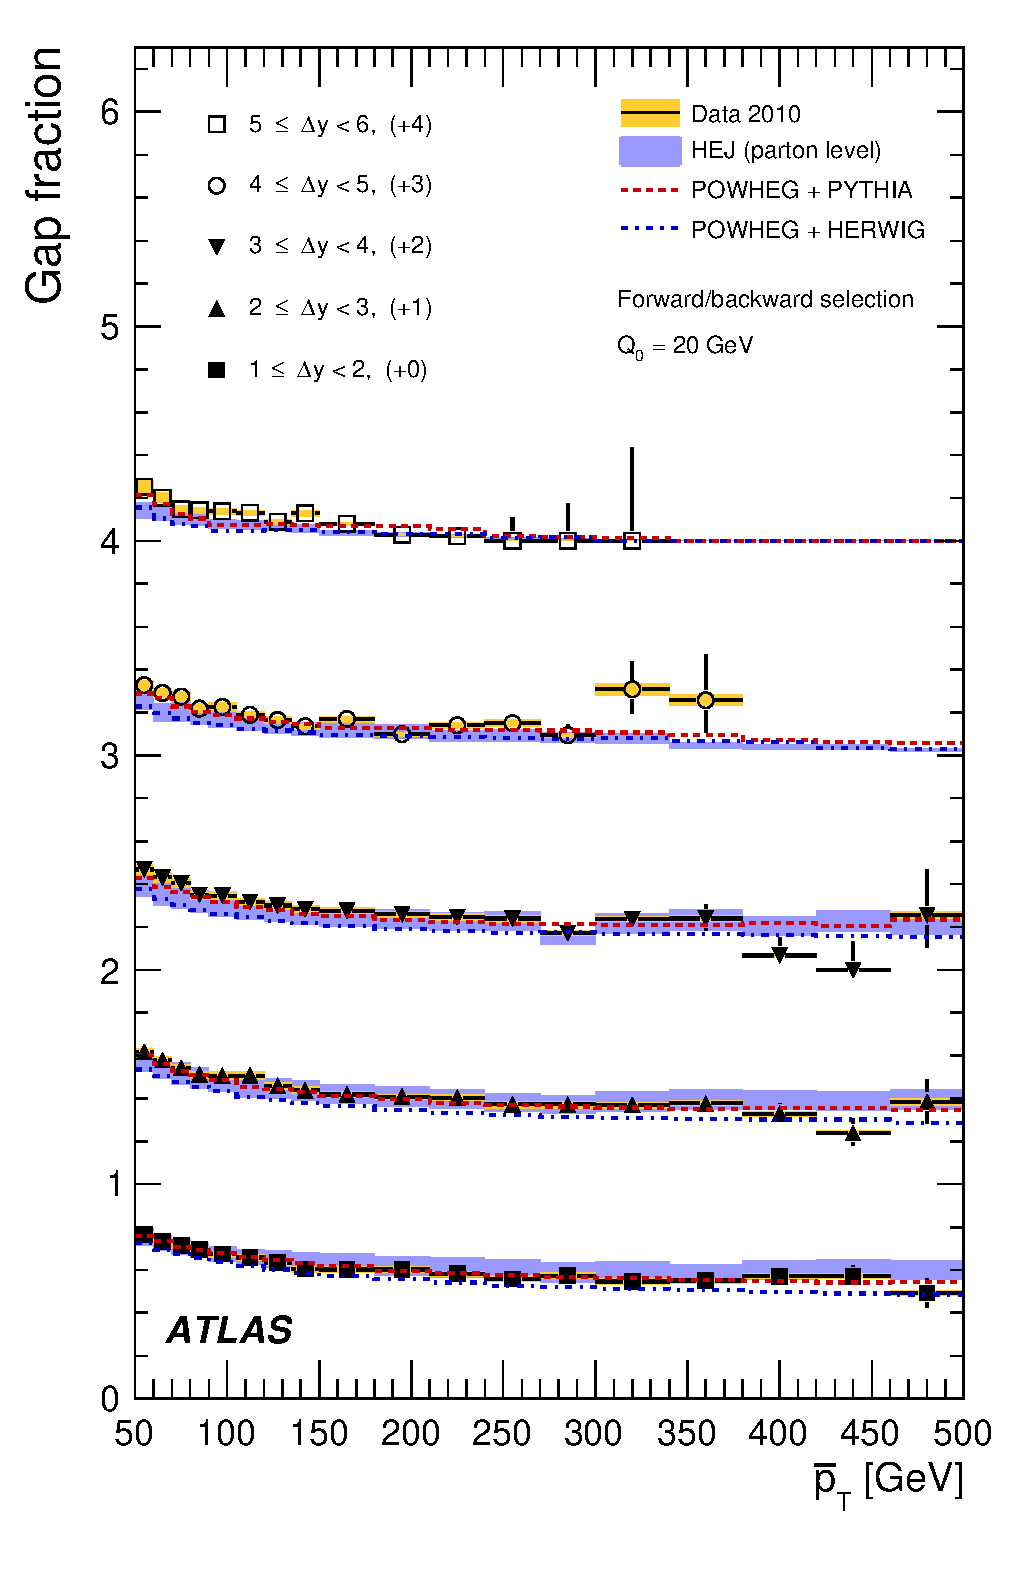
\includegraphics[width=\smallfigwidth]{chapters/gbj/GapFraction_PtBarDist_gap_Q0_sel_B.eps}
    \label{fig:gbj:Gap_fraction_pTbar_B_comparison}}
  \quad
  \subfloat[Ratio to theory]{
    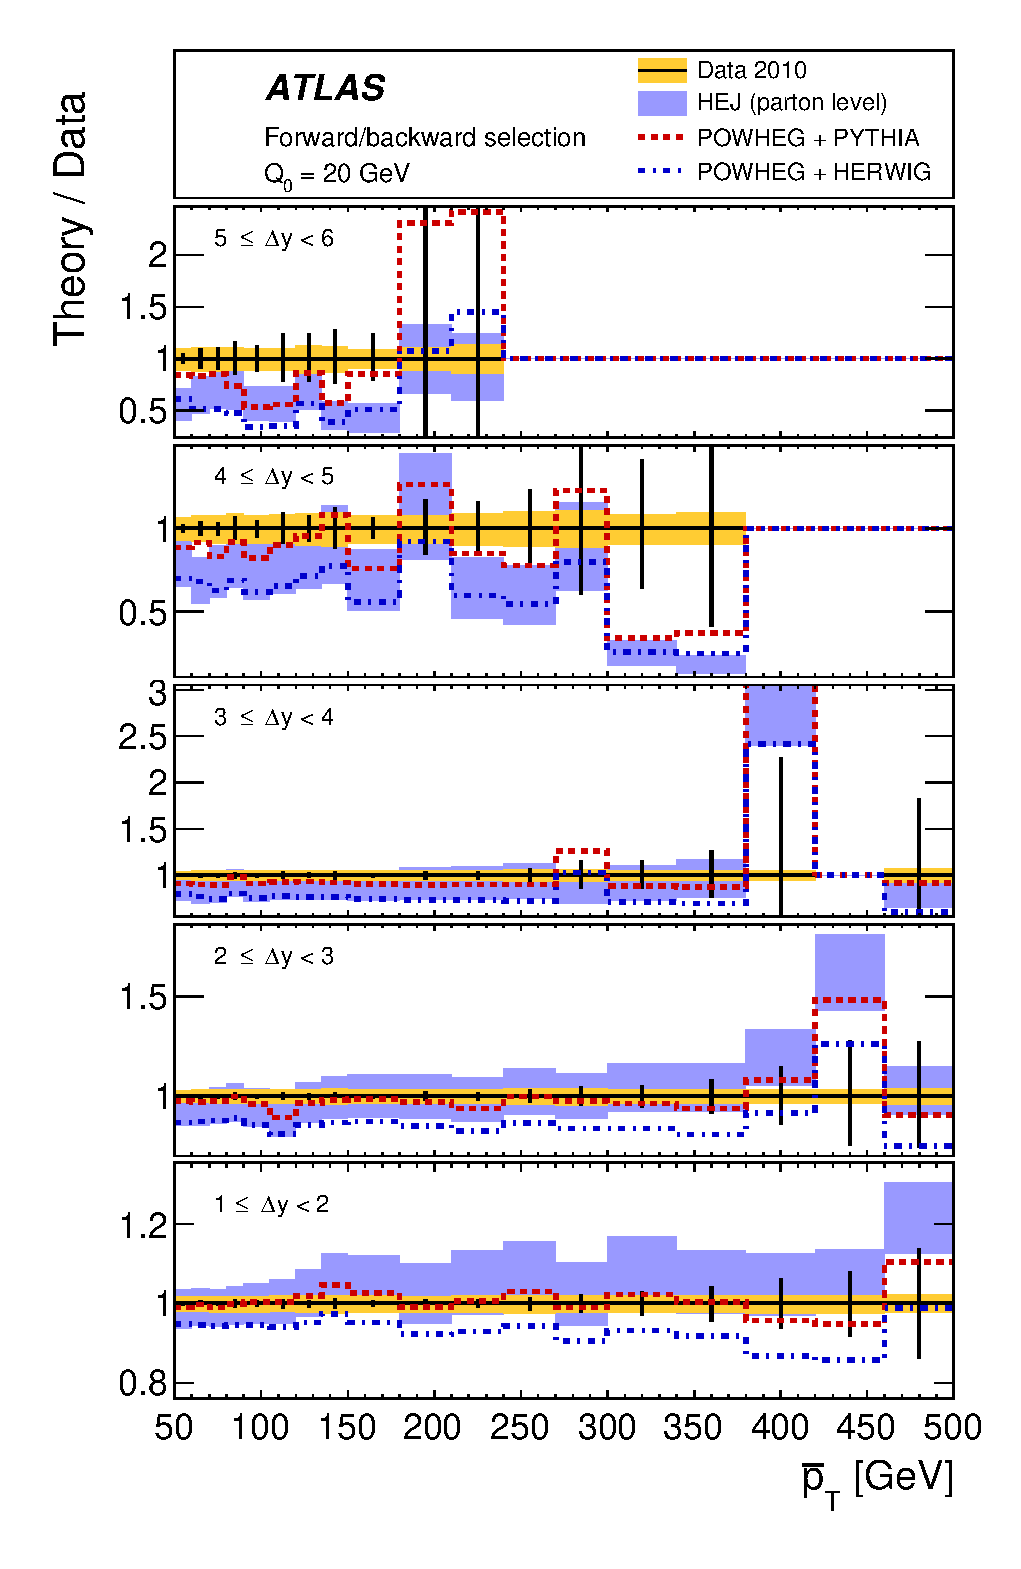
\includegraphics[width=\smallfigwidth]{chapters/gbj/GapFraction_PtBarDist_gap_Q0_sel_B_Ratio.eps}
    \label{fig:gbj:Gap_fraction_pTbar_B_ratio}}
  \caption{Gap fraction as a function of \pTbar for five \DeltaY slices. \protect\subref{fig:gbj:Gap_fraction_pTbar_B_comparison}
           shows selection B data against the \HEJ and \Powheg generators, while \protect\subref{fig:gbj:Gap_fraction_pTbar_B_ratio}
           shows the ratio of the theory predictions to the data. The data and theory
           are presented in the same way as \FigureRef{fig:gbj:Gap_fraction_pTbar_A}.}
  \label{fig:gbj:Gap_fraction_pTbar_B}
\end{figure}

\FiguresRef{fig:gbj:Gap_fraction_pTbar_A}{fig:gbj:Gap_fraction_pTbar_B} show the
gap fraction as a function of \pTbar for selections A and B, respectively. A particularly striking feature
is that the parton level \HEJ prediction, based on \BFKL resummation, predicts too
little jet activity, and hence too large a gap fraction, at large values of $\pTbar / \Qnought$
for selection A. For selection B, however, the \HEJ prediction shows much better
agreement with the data; this behaviour is expected since the \HEJ formalism assumes
a large rapidity gap between the boundary jets.

\begin{figure}[htpb]
  \subfloat[\pTbar slices]{
    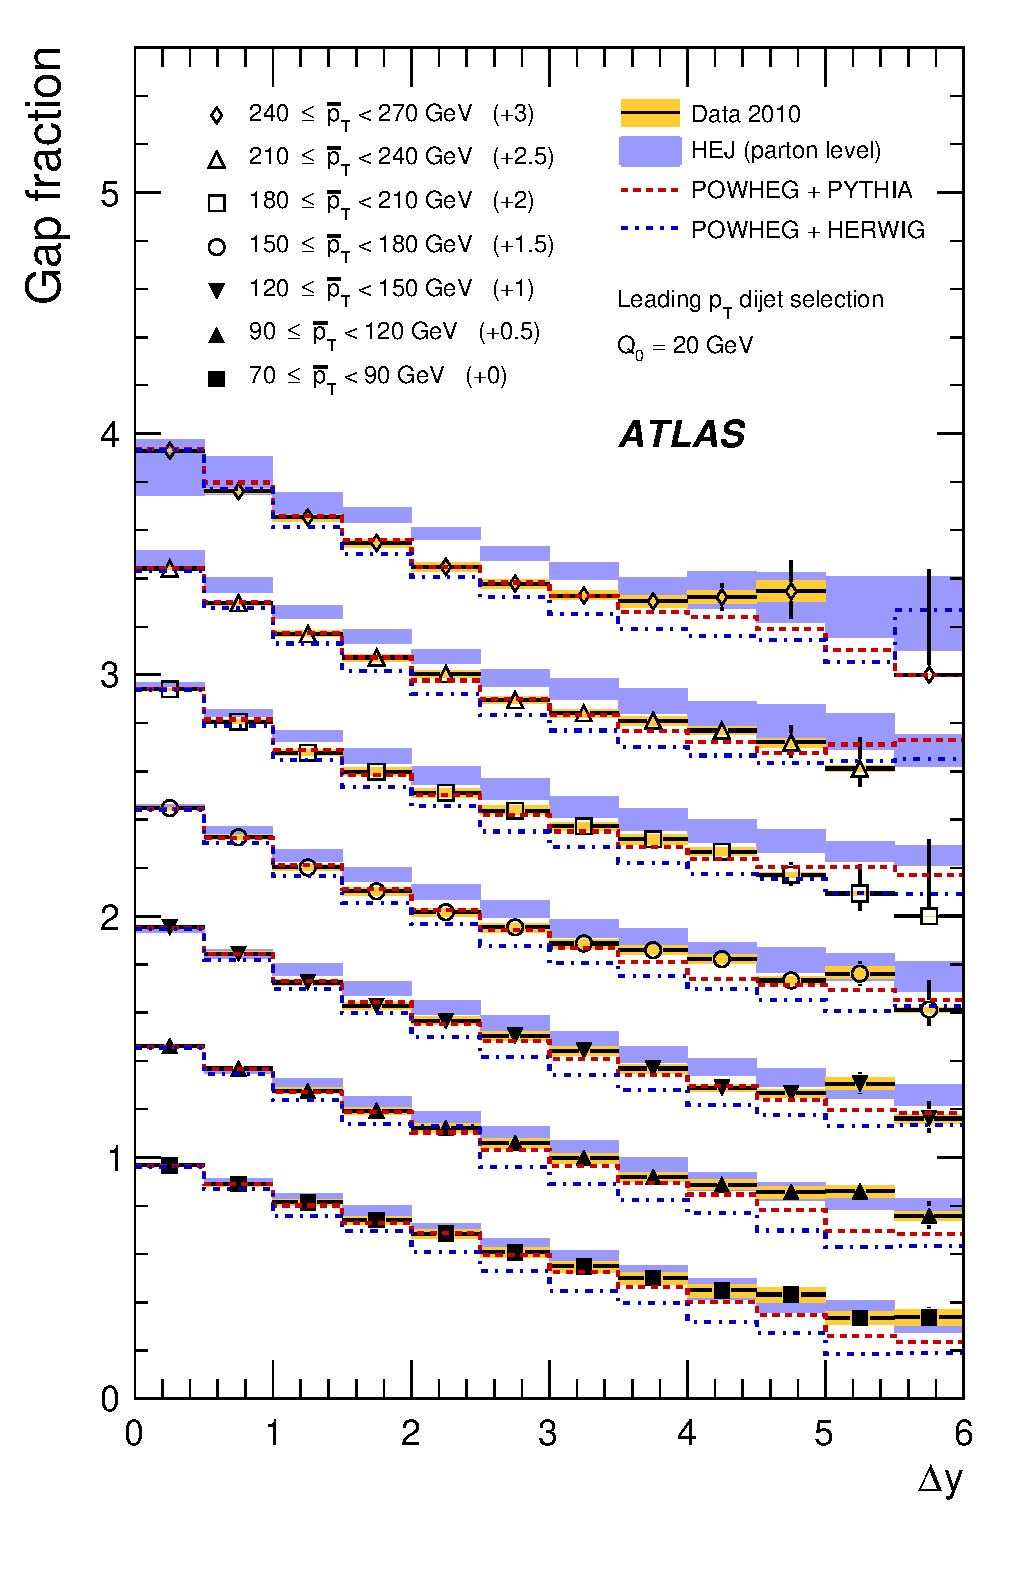
\includegraphics[width=\smallfigwidth]{chapters/gbj/GapFraction_YDist_gap_Q0_sel_A.eps}
    \label{fig:gbj:Gap_fraction_dY_A_comparison}}
  \quad
  \subfloat[Ratio to theory]{
    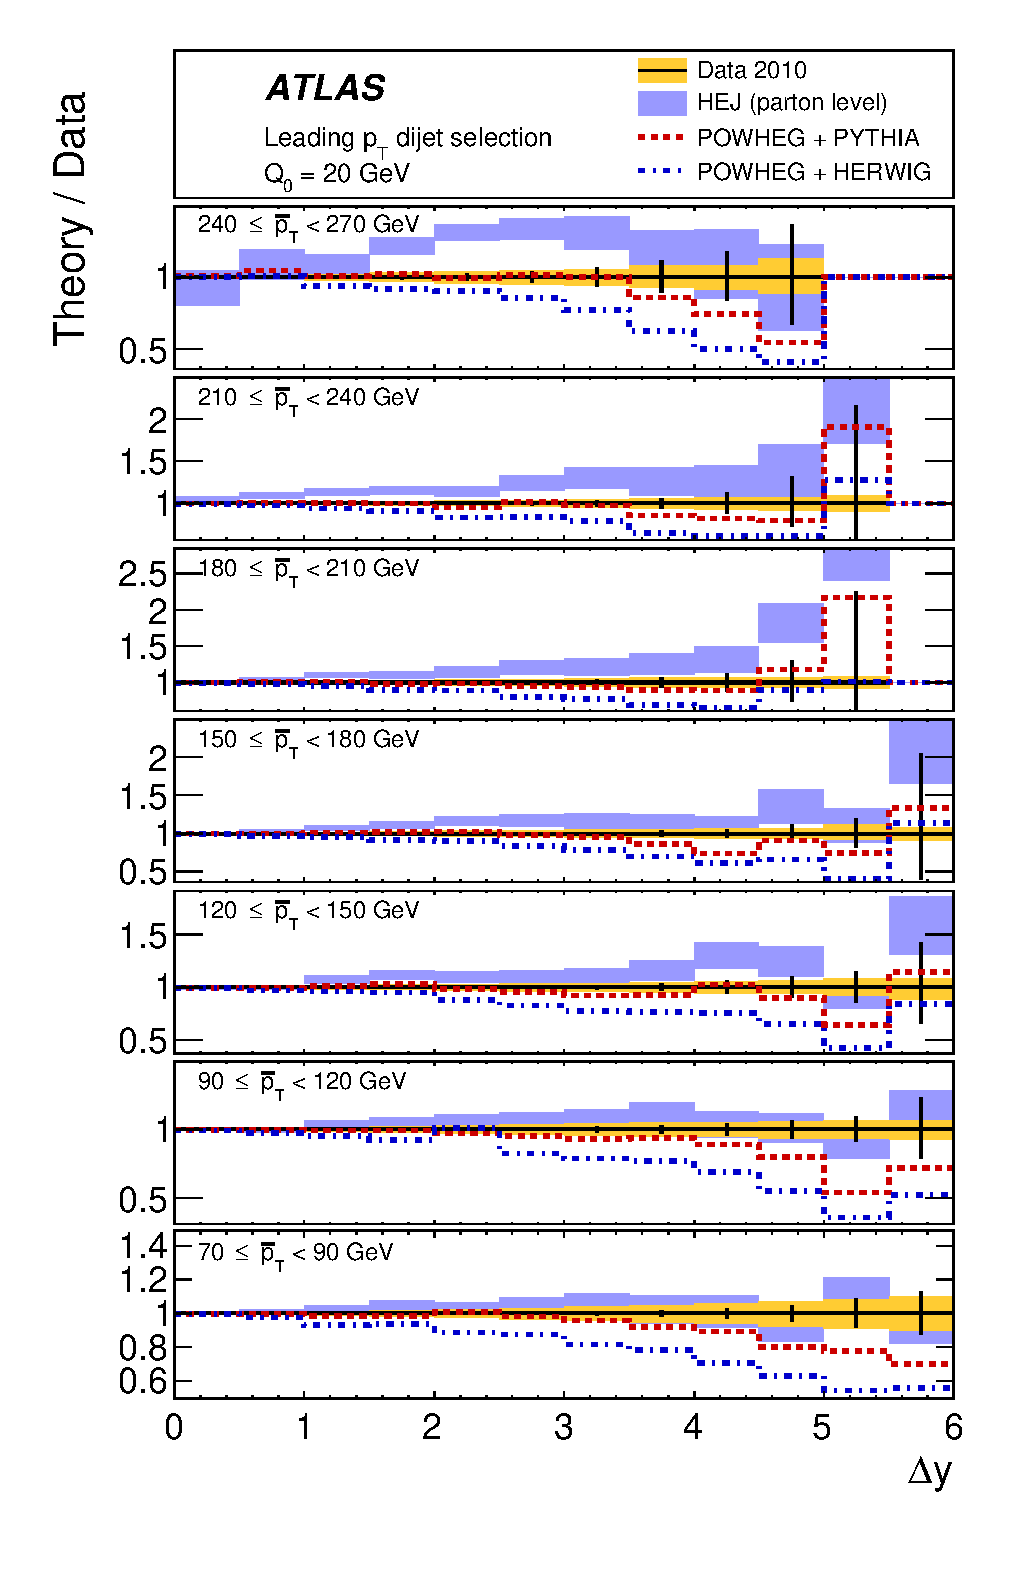
\includegraphics[width=\smallfigwidth]{chapters/gbj/GapFraction_YDist_gap_Q0_sel_A_Ratio.eps}
    \label{fig:gbj:Gap_fraction_dY_A_ratio}}
  \caption{Gap fraction as a function of \DeltaY for seven \pTbar slices. \protect\subref{fig:gbj:Gap_fraction_dY_A_comparison}
           shows selection A data against the \HEJ and \Powheg generators, while \protect\subref{fig:gbj:Gap_fraction_dY_A_ratio}
           shows the ratio of the theory predictions to the data. The data and theory
           are presented in the same way as \FigureRef{fig:gbj:Gap_fraction_pTbar_A}.}
  \label{fig:gbj:Gap_fraction_dY_A}
\end{figure}

\begin{figure}[htpb]
  \subfloat[\pTbar slices]{
    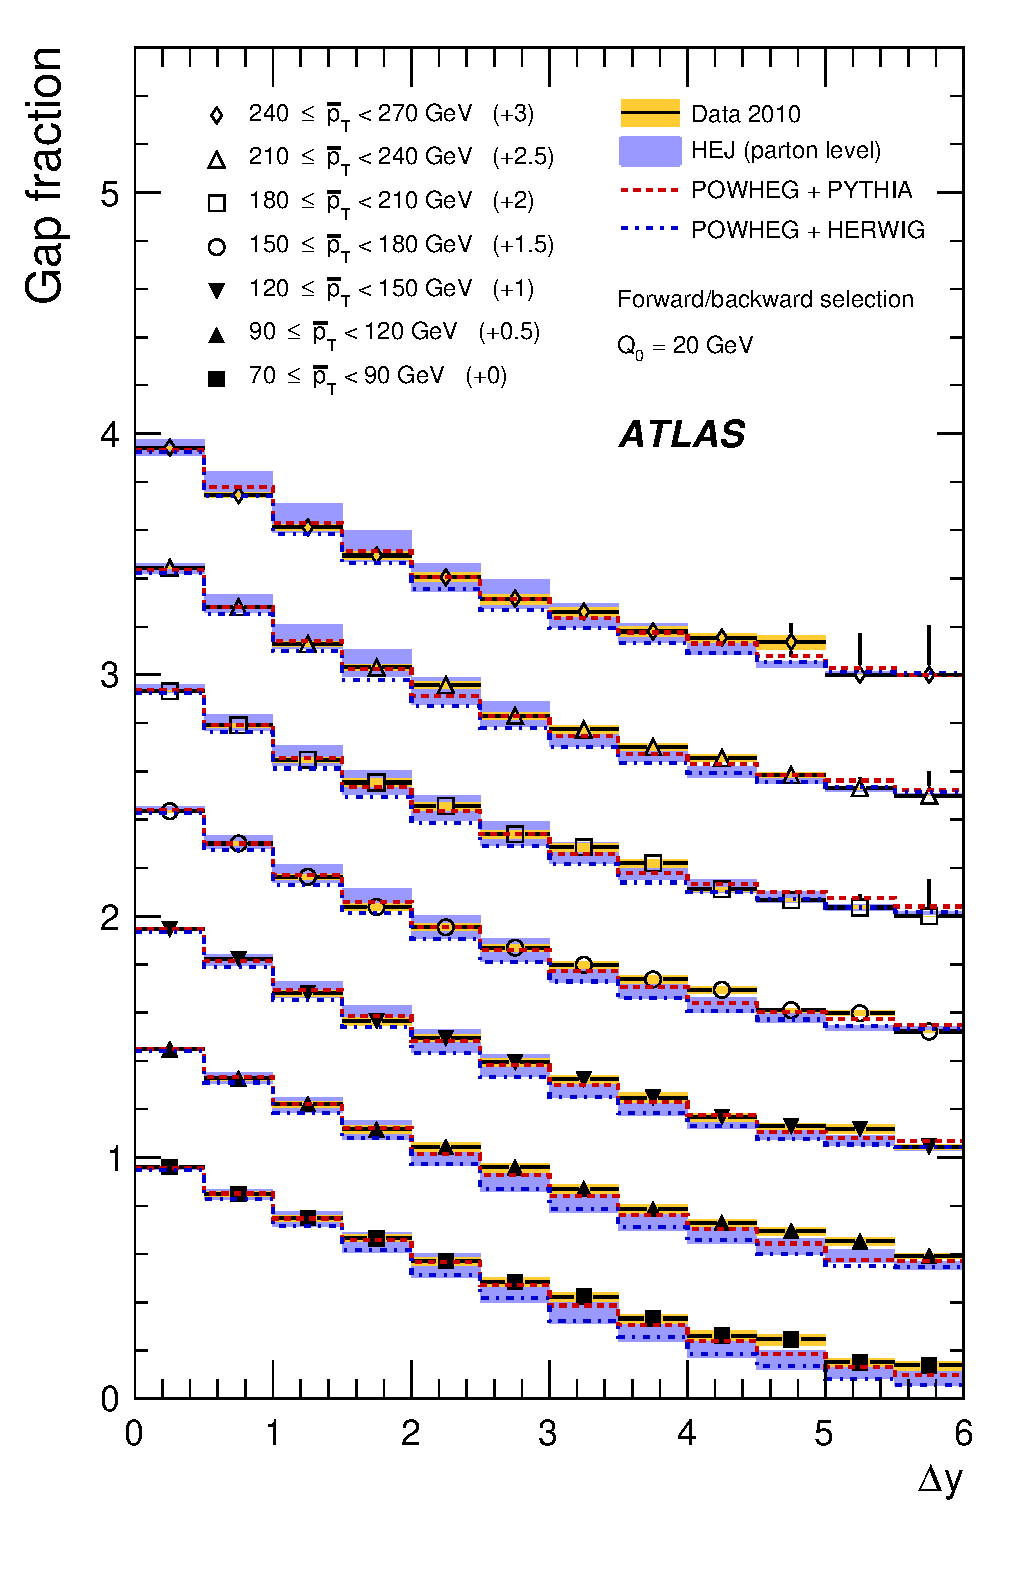
\includegraphics[width=\smallfigwidth]{chapters/gbj/GapFraction_YDist_gap_Q0_sel_B.eps}
    \label{fig:gbj:Gap_fraction_dY_B_comparison}}
  \quad
  \subfloat[Ratio to theory]{
    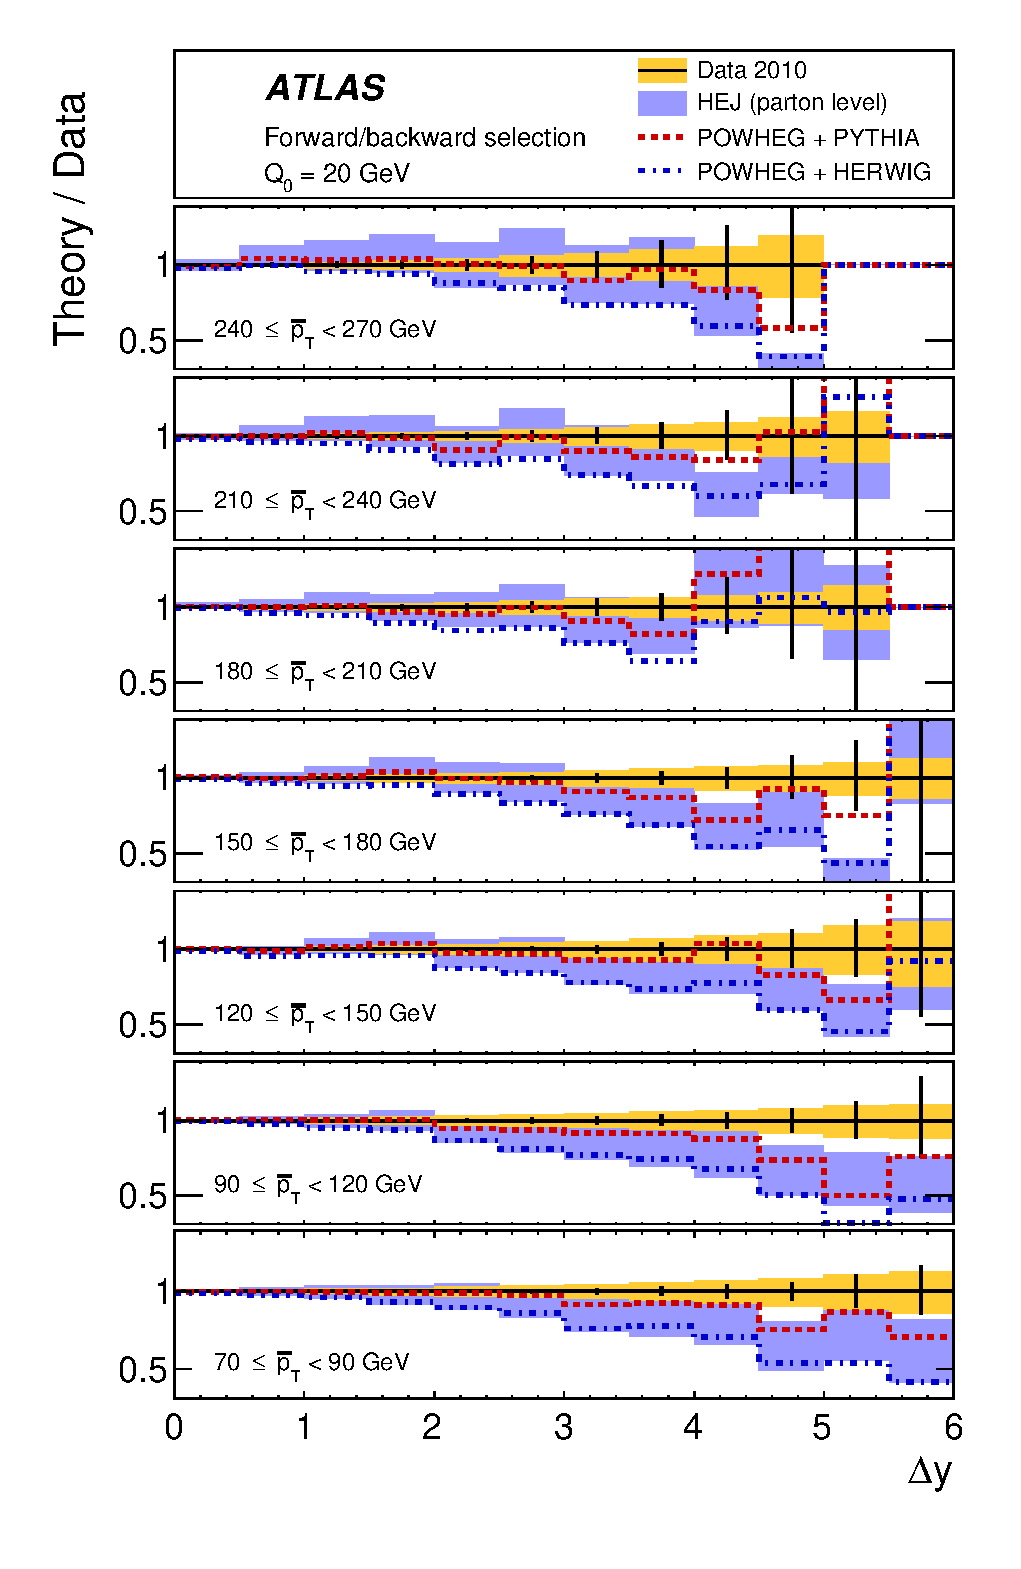
\includegraphics[width=\smallfigwidth]{chapters/gbj/GapFraction_YDist_gap_Q0_sel_B_Ratio.eps}
    \label{fig:gbj:Gap_fraction_dY_B_ratio}}
  \caption{Gap fraction as a function of \DeltaY for seven \pTbar slices. \protect\subref{fig:gbj:Gap_fraction_dY_B_comparison}
           shows selection B data against the \HEJ and \Powheg generators, while \protect\subref{fig:gbj:Gap_fraction_dY_B_ratio}
           shows the ratio of the theory predictions to the data. The data and theory
           are presented in the same way as \FigureRef{fig:gbj:Gap_fraction_pTbar_A}.}
  \label{fig:gbj:Gap_fraction_dY_B}
\end{figure}

\FiguresRef{fig:gbj:Gap_fraction_dY_A}{fig:gbj:Gap_fraction_dY_B} show the gap
fraction as a function of \DeltaY. Again, the \HEJ prediction deviates from the
data, here specifying too much jet activity, and so too low a gap fraction at
large \DeltaY when the boundary jets are selected as the most forward and most backward jets in the event. 

\begin{figure}[htpb]
  \subfloat[\pTbar and \DeltaY slices]{
    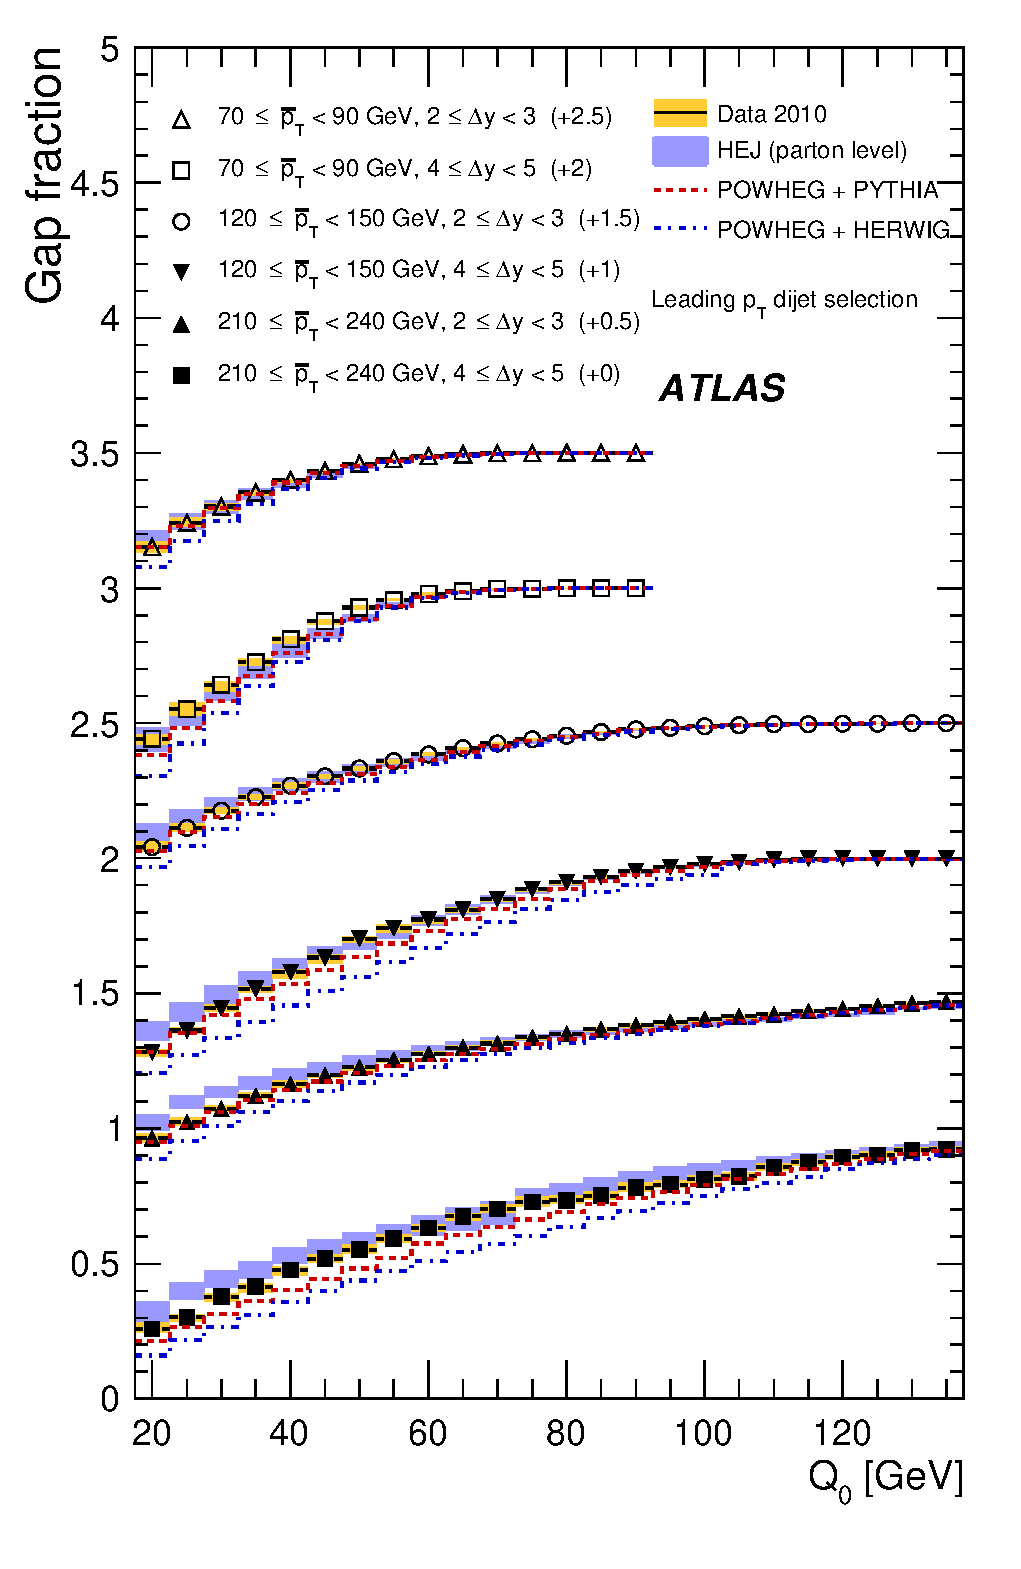
\includegraphics[width=\smallfigwidth]{chapters/gbj/GapFraction_Q0Dist_gap_sel_A.eps}
    \label{fig:gbj:Gap_fraction_Q0_A_comparison}}
  \quad
  \subfloat[Ratio to theory]{
    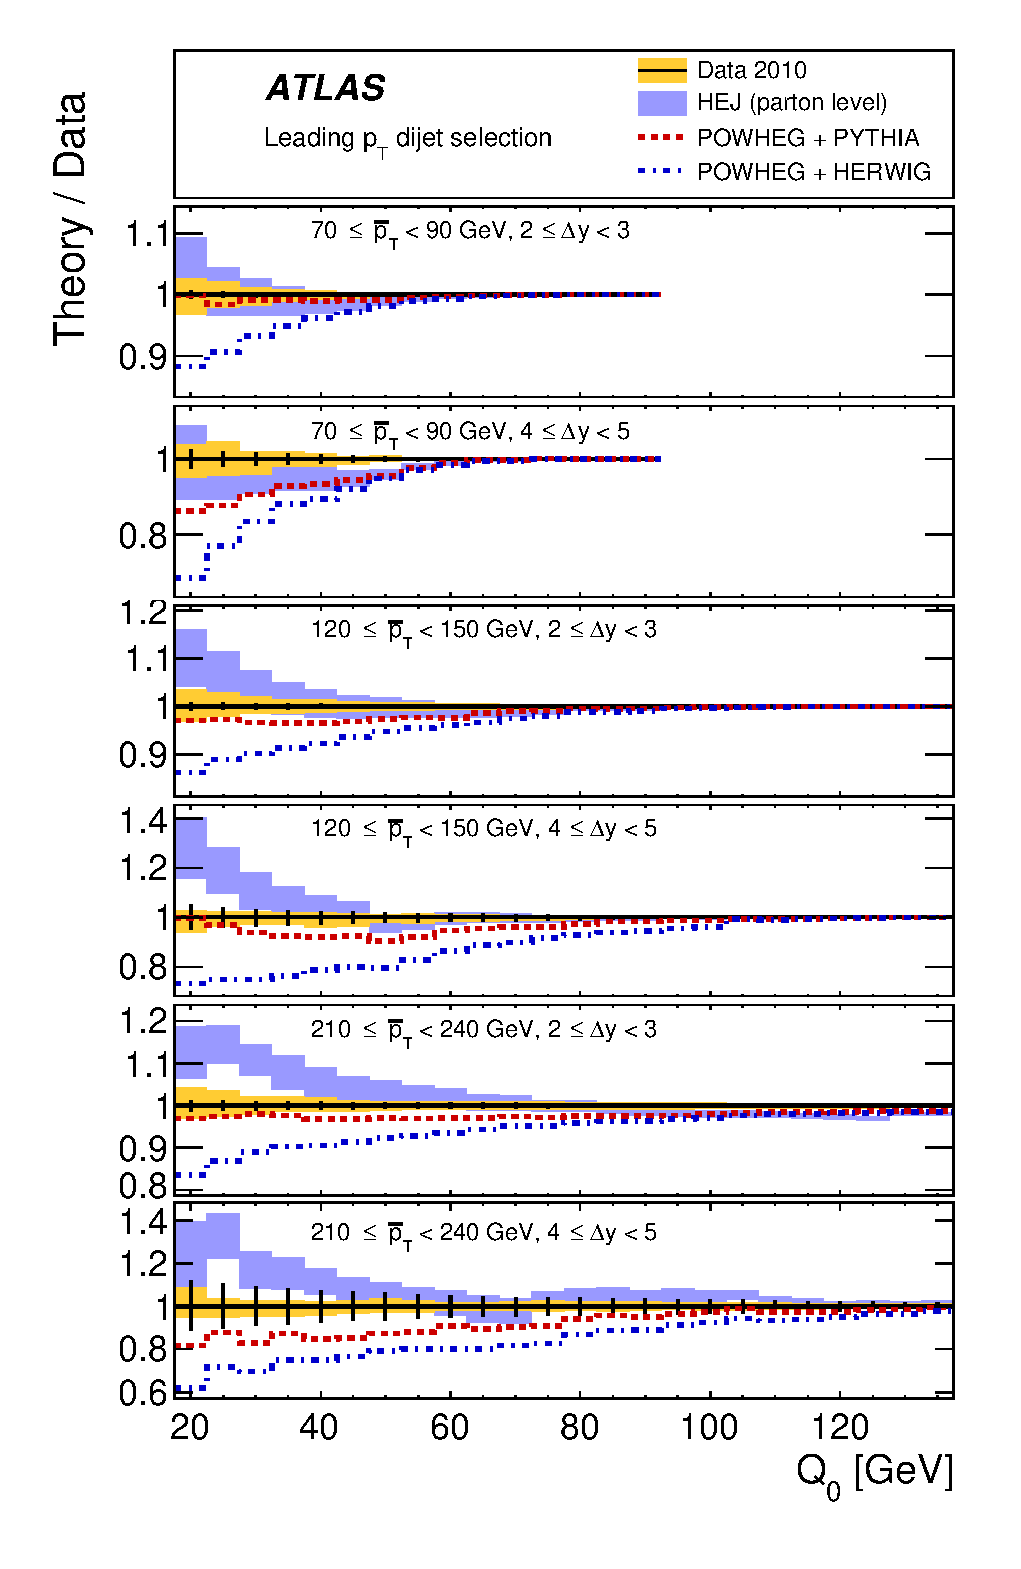
\includegraphics[width=\smallfigwidth]{chapters/gbj/GapFraction_Q0Dist_gap_sel_A_Ratio.eps}
    \label{fig:gbj:Gap_fraction_Q0_A_ratio}}
  \caption{Gap fraction as a function of \Qnought for six different \pTbar and \DeltaY
           slices. \protect\subref{fig:gbj:Gap_fraction_Q0_A_comparison} shows selection
           A data against the \HEJ and \Powheg generators, while \protect\subref{fig:gbj:Gap_fraction_Q0_A_ratio}
           shows the ratio of the theory predictions to the data. The data points for $\Qnought > \pTbar$ have been
           removed because the gap fraction is always equal to one for this
           \dijet selection, by definition. The data and theory are presented in
           the same way as \FigureRef{fig:gbj:Gap_fraction_pTbar_A}.}
  \label{fig:gbj:Gap_fraction_Q0_A}
\end{figure}

\begin{figure}[htpb]
  \subfloat[\DeltaY slices]{
    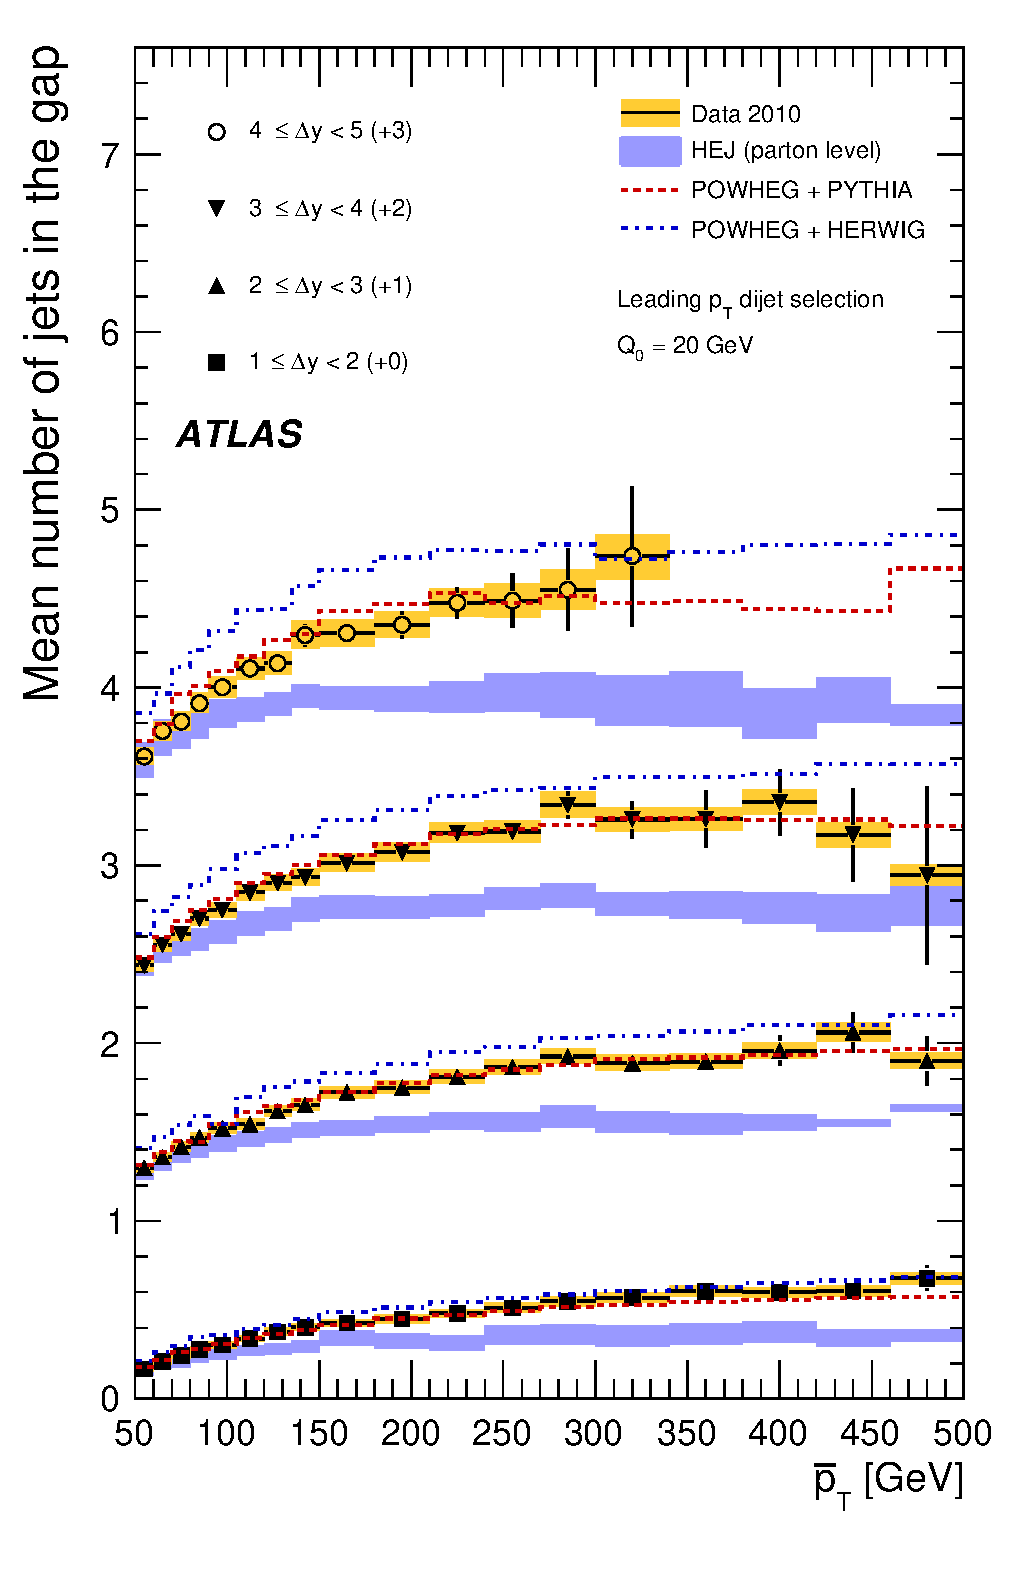
\includegraphics[width=\smallfigwidth]{chapters/gbj/Njet_PtBarDist_gap_Q0_sel_A.eps}
    \label{fig:gbj:N_jets_pTbar_A_comparison}}
  \quad
  \subfloat[Ratio to theory]{
    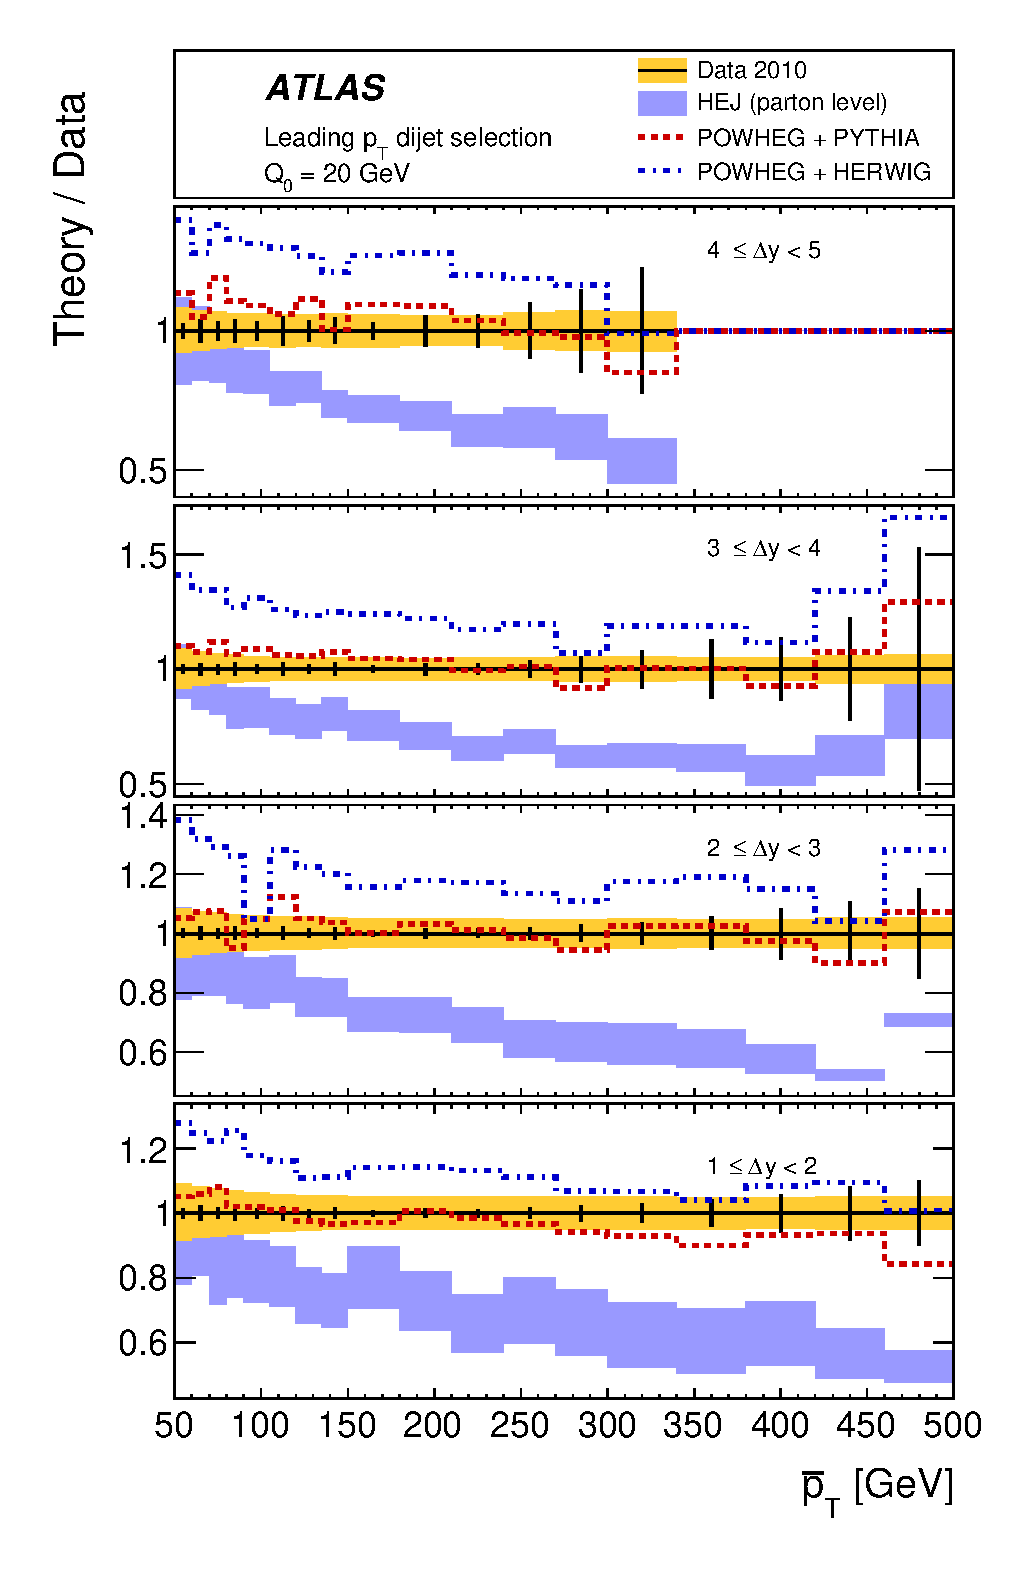
\includegraphics[width=\smallfigwidth]{chapters/gbj/Njet_PtBarDist_gap_Q0_sel_A_Ratio.eps}
    \label{fig:gbj:N_jets_pTbar_A_ratio}}
  \caption{Mean number of jets in the gap as a function of \pTbar for four \DeltaY
           slices. \protect\subref{fig:gbj:N_jets_pTbar_A_comparison} shows selection
           A data against the \HEJ and \Powheg generators, while \protect\subref{fig:gbj:N_jets_pTbar_A_ratio}
           shows the ratio of the theory predictions to the data. The data and theory
           are presented in the same way as \FigureRef{fig:gbj:Gap_fraction_pTbar_A}.}
  \label{fig:gbj:N_jets_pTbar_A}
\end{figure}

\begin{figure}[htpb]
  \subfloat[\DeltaY slices]{
    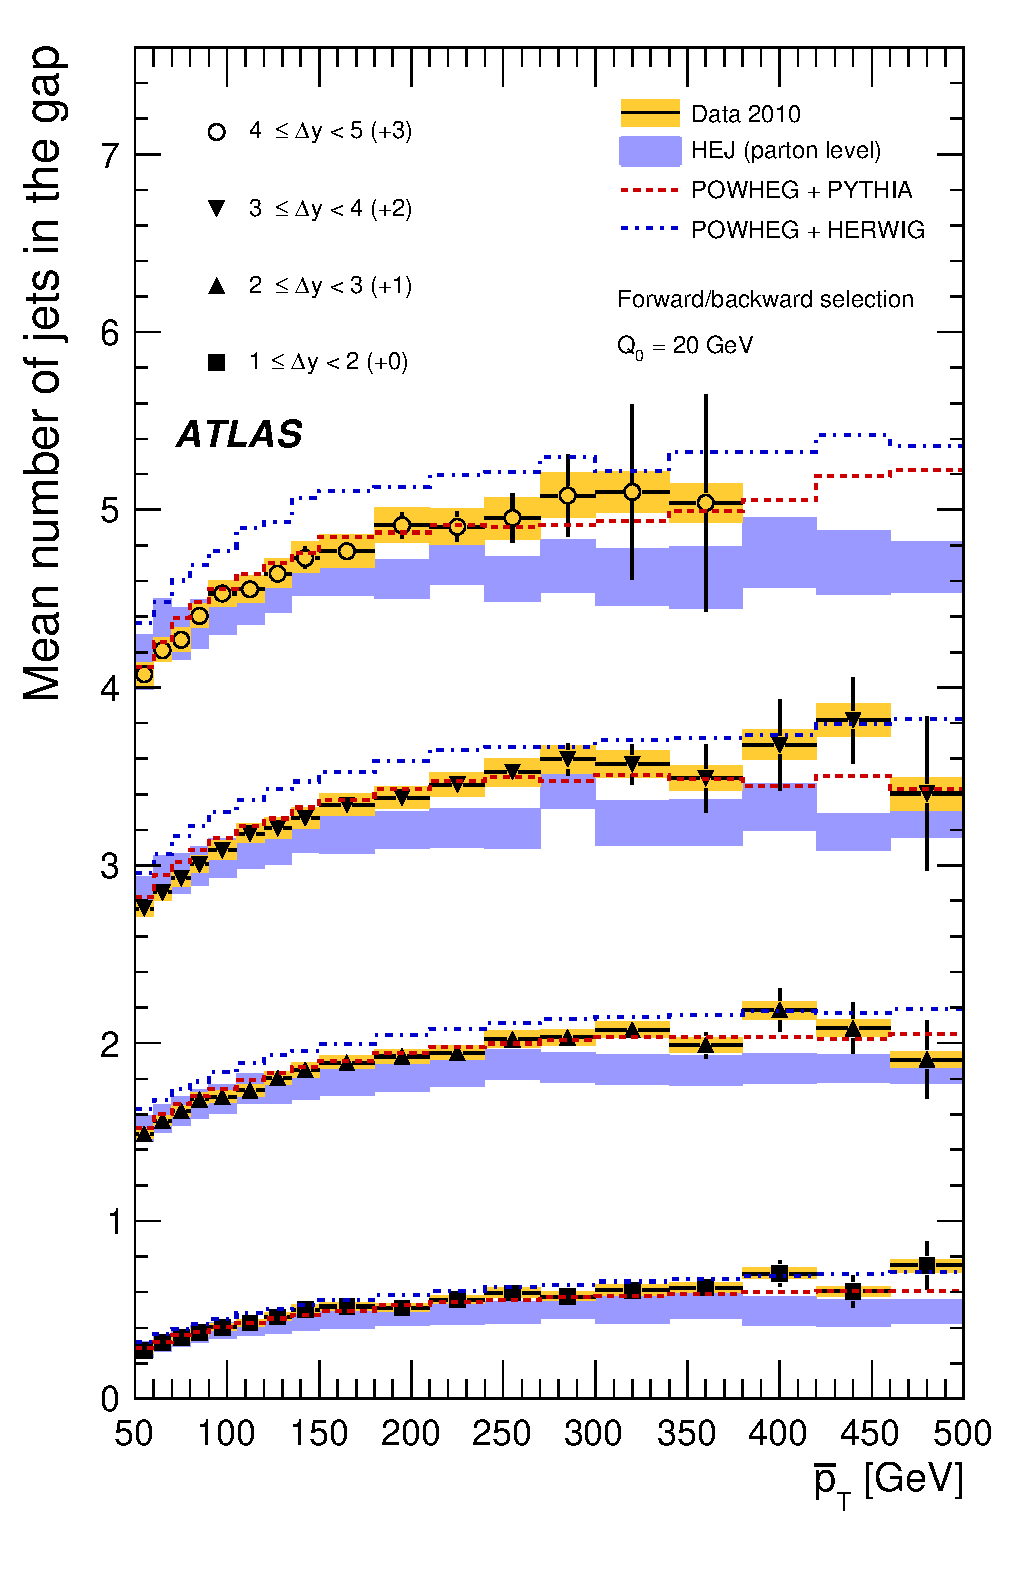
\includegraphics[width=\smallfigwidth]{chapters/gbj/Njet_PtBarDist_gap_Q0_sel_B.eps}
    \label{fig:gbj:N_jets_pTbar_B_comparison}}
  \quad
  \subfloat[Ratio to theory]{
    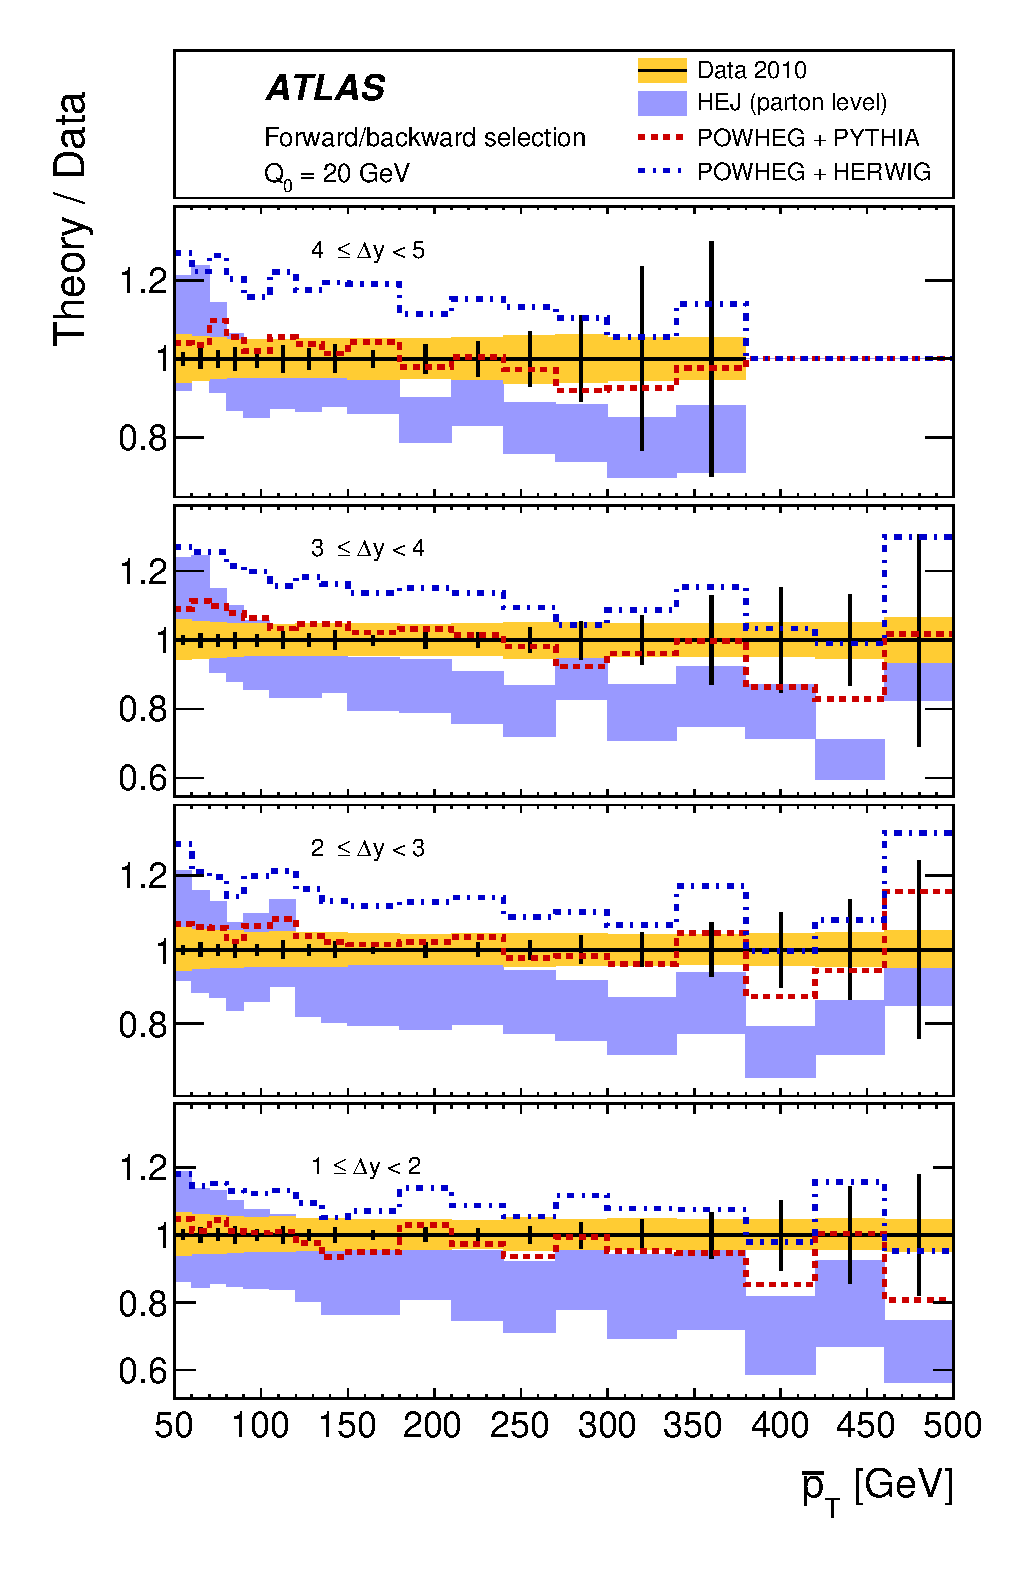
\includegraphics[width=\smallfigwidth]{chapters/gbj/Njet_PtBarDist_gap_Q0_sel_B_Ratio.eps}
    \label{fig:gbj:N_jets_pTbar_B_ratio}}
  \caption{Mean number of jets in the gap as a function of \pTbar for four \DeltaY
           slices. \protect\subref{fig:gbj:N_jets_pTbar_B_comparison} shows selection
           B data against the \HEJ and \Powheg generators, while \protect\subref{fig:gbj:N_jets_pTbar_B_ratio}
           shows the ratio of the theory predictions to the data. The data and theory
           are presented in the same way as \FigureRef{fig:gbj:Gap_fraction_pTbar_A}.}
  \label{fig:gbj:N_jets_pTbar_B}
\end{figure}

\FigureRef{fig:gbj:Gap_fraction_Q0_A} shows the gap fraction as a function of
the veto scale, \Qnought for selection A data. \FiguresRef{fig:gbj:N_jets_pTbar_A}{fig:gbj:N_jets_pTbar_B} show the mean
number of jets in the gap region as a function of \pTbar for selections A and B,
respectively. Again \HEJ can be seen to perform poorly at high \pTbar and high
\DeltaY.

\begin{figure}[htpb]
  \subfloat[\pTbar slices]{
    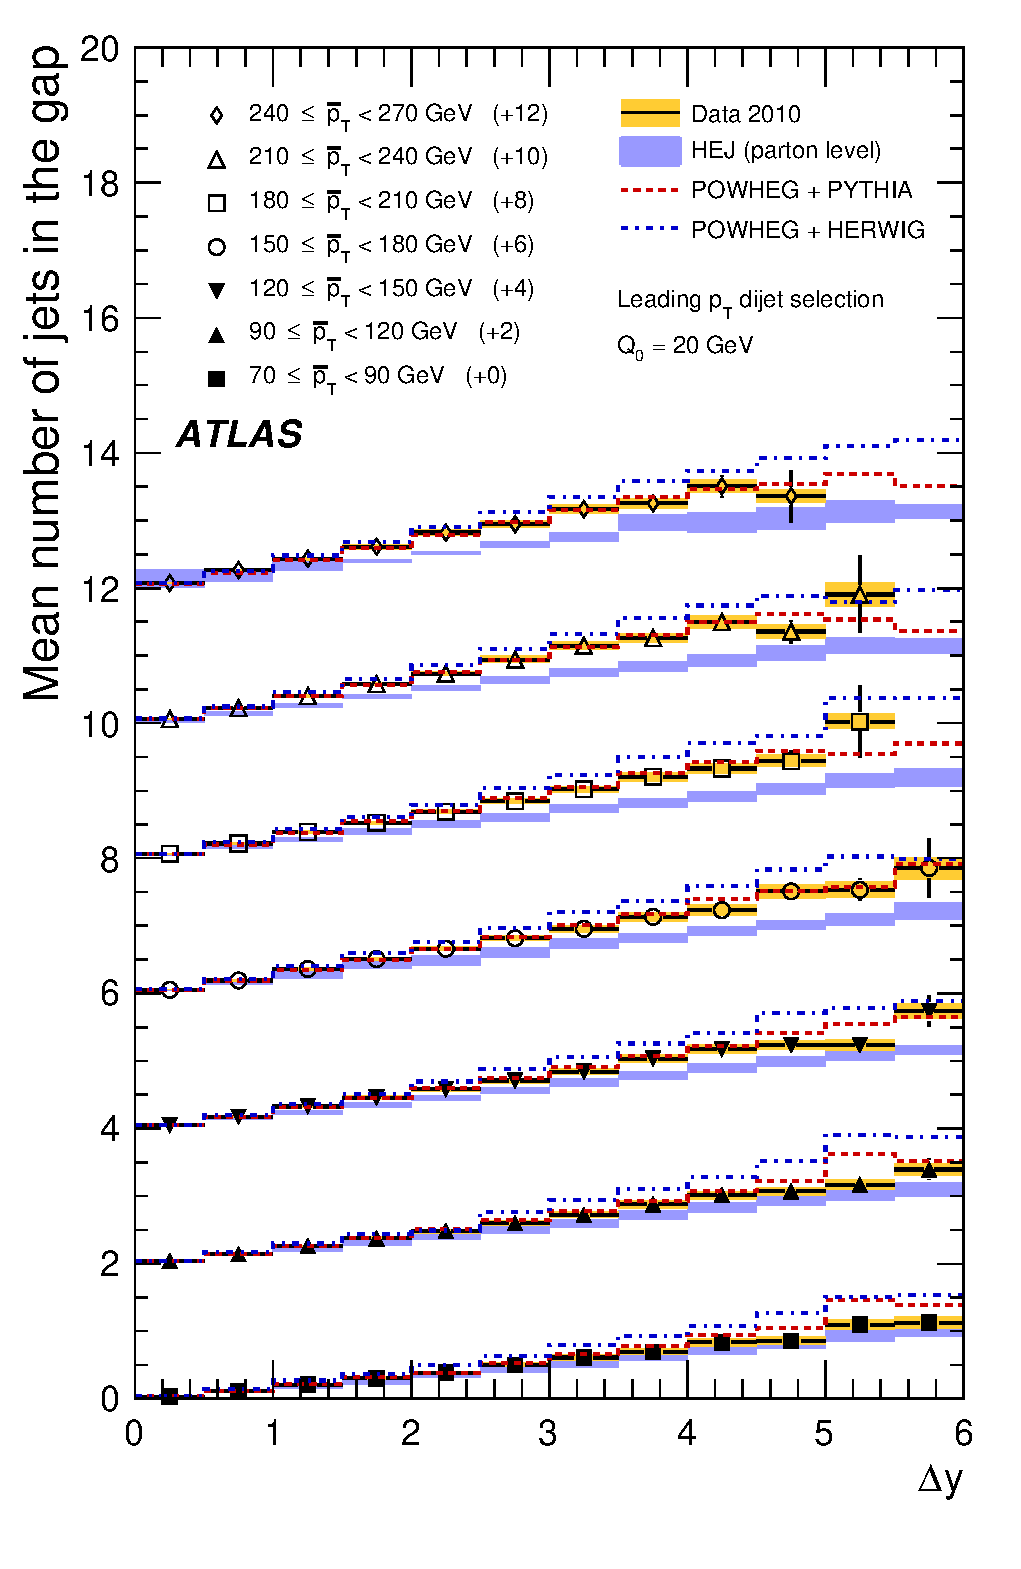
\includegraphics[width=\smallfigwidth]{chapters/gbj/Njet_YDist_gap_Q0_sel_A.eps}
    \label{fig:gbj:N_jets_dY_A_comparison}}
  \quad
  \subfloat[Ratio to theory]{
    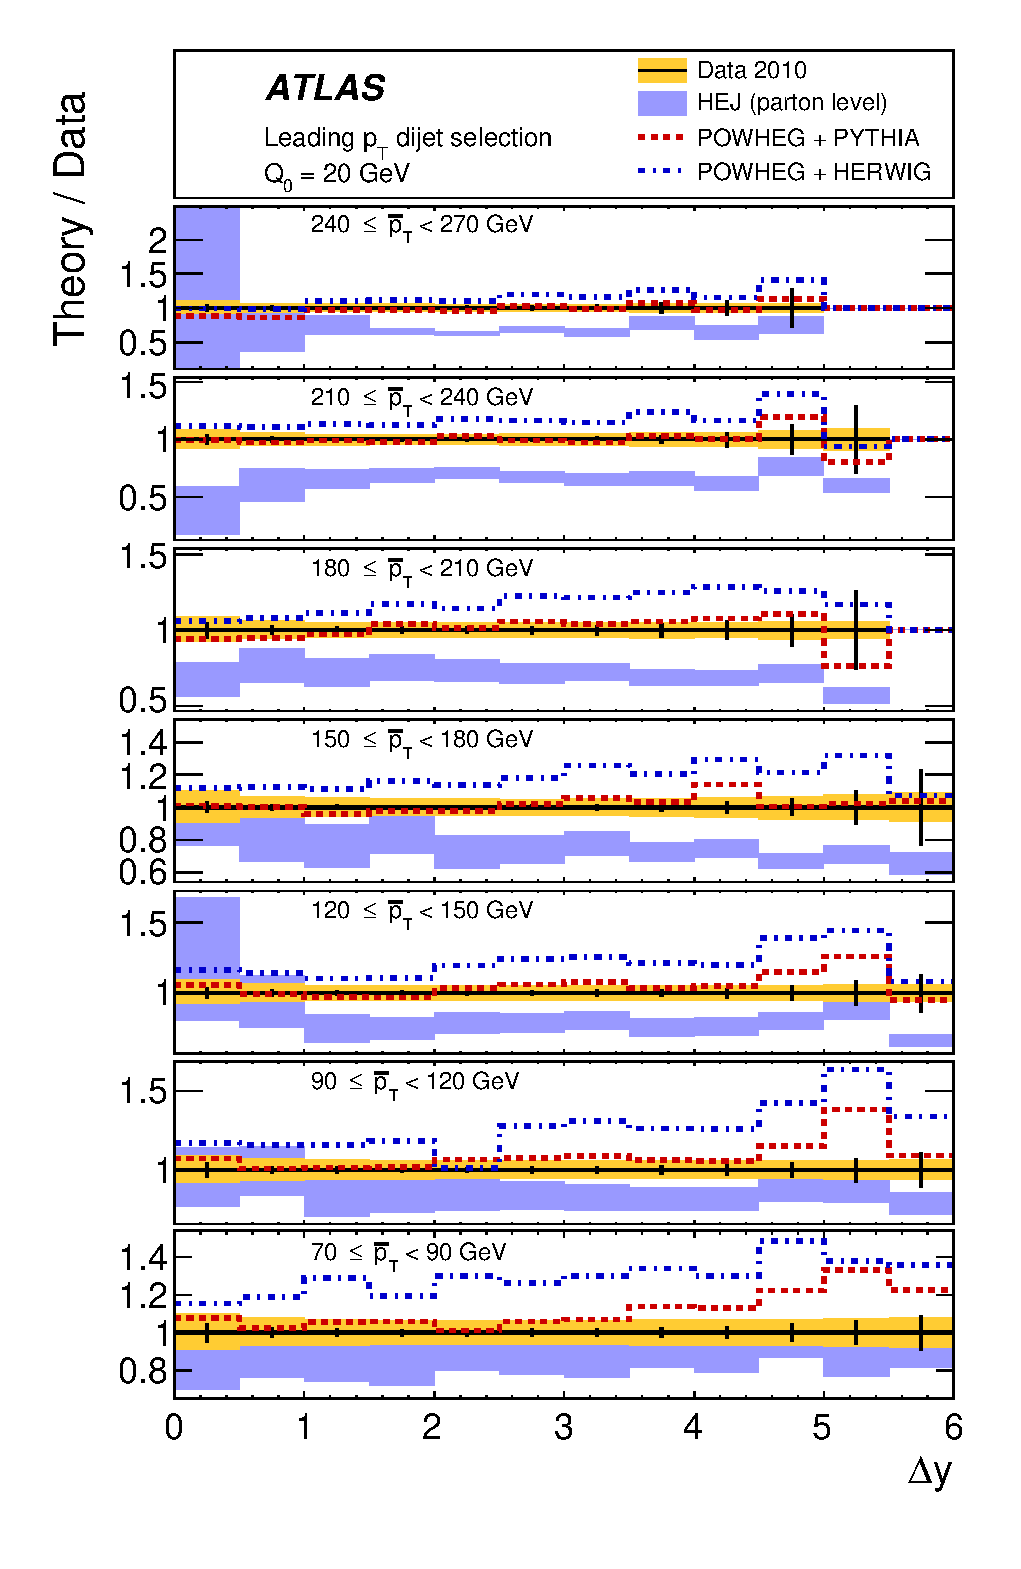
\includegraphics[width=\smallfigwidth]{chapters/gbj/Njet_YDist_gap_Q0_sel_A_Ratio.eps}
    \label{fig:gbj:N_jets_dY_A_ratio}}
  \caption{Mean number of jets in the gap as a function of \DeltaY for seven \pTbar
           slices. \protect\subref{fig:gbj:N_jets_dY_A_comparison} shows selection
           A data against the \HEJ and \Powheg generators, while \protect\subref{fig:gbj:N_jets_dY_A_ratio}
           shows the ratio of the theory predictions to the data. The data and theory
           are presented in the same way as \FigureRef{fig:gbj:Gap_fraction_pTbar_A}.}
  \label{fig:gbj:N_jets_dY_A}
\end{figure}

\begin{figure}[htpb]
  \subfloat[\pTbar slices]{
    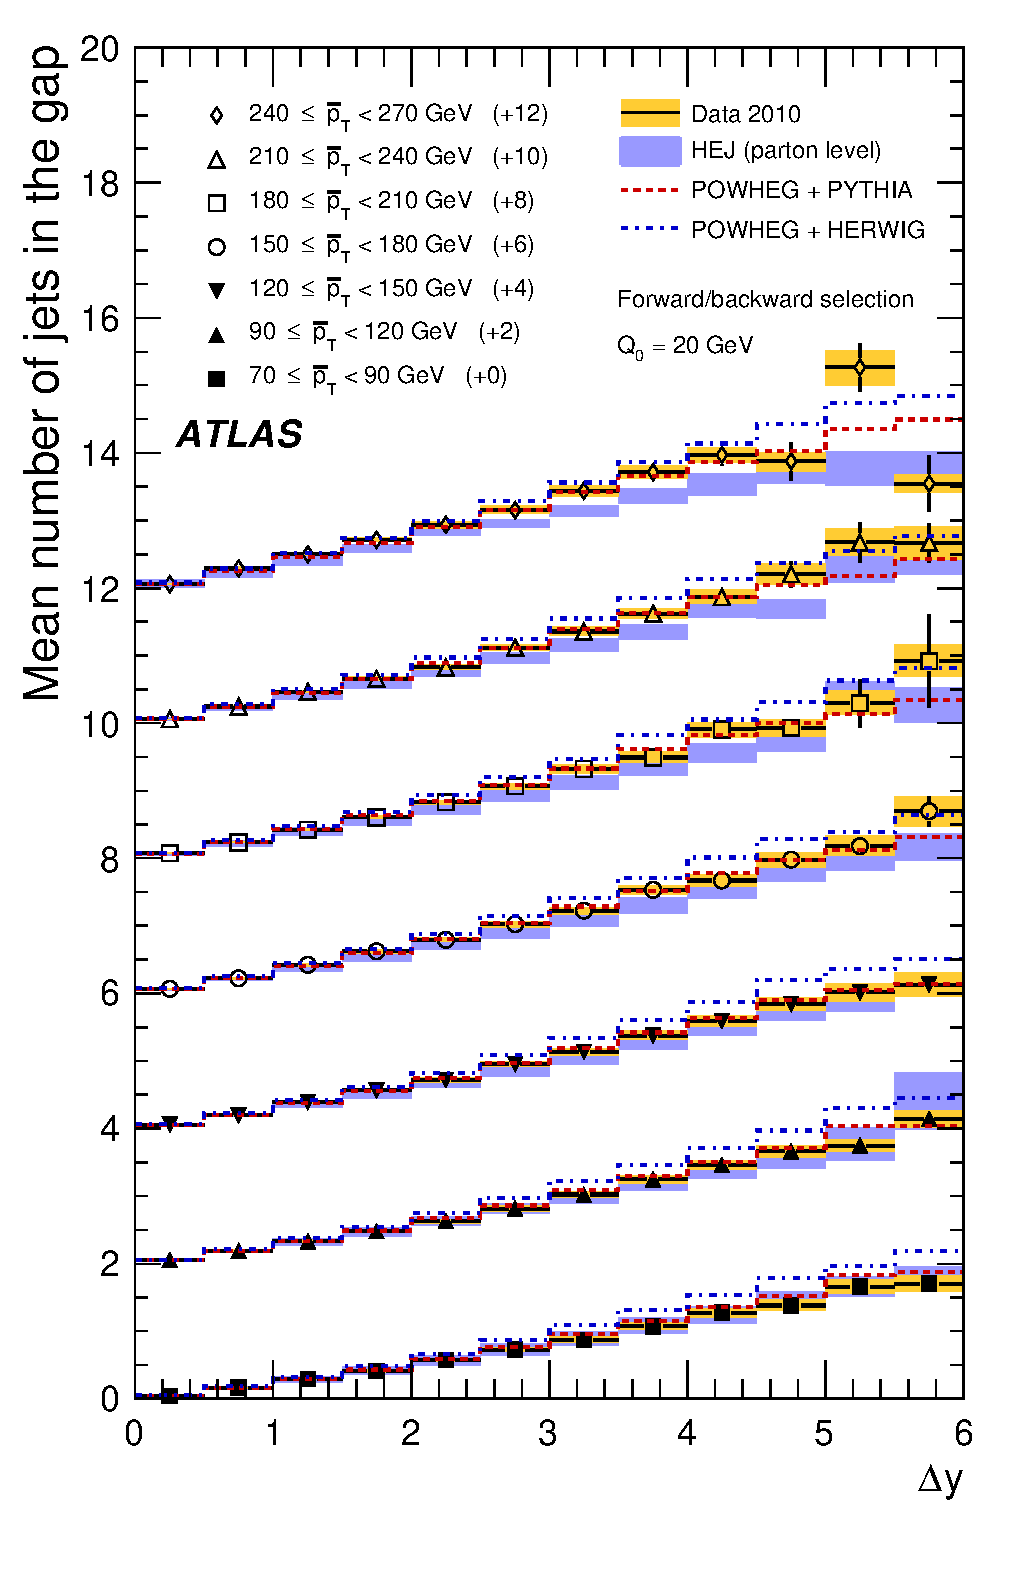
\includegraphics[width=\smallfigwidth]{chapters/gbj/Njet_YDist_gap_Q0_sel_B.eps}
    \label{fig:gbj:N_jets_dY_B_comparison}}
  \quad
  \subfloat[Ratio to theory]{
    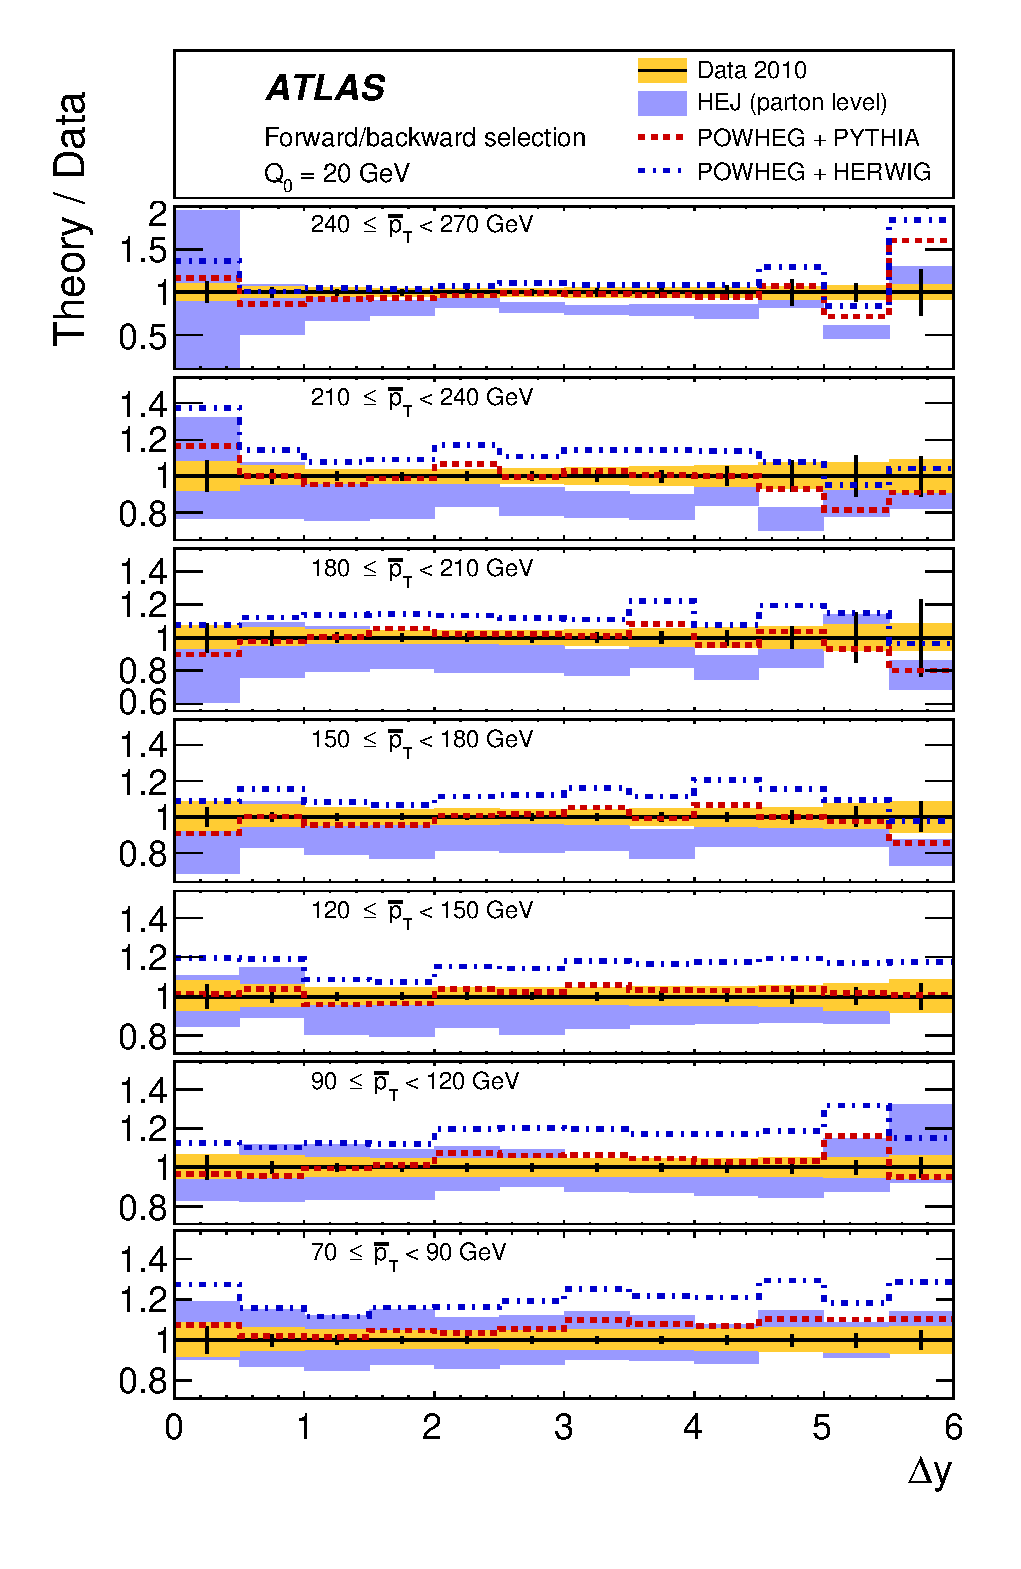
\includegraphics[width=\smallfigwidth]{chapters/gbj/Njet_YDist_gap_Q0_sel_B_Ratio.eps}
    \label{fig:gbj:N_jets_dY_B_ratio}}
  \caption{Mean number of jets in the gap as a function of \DeltaY for seven \pTbar
           slices. \protect\subref{fig:gbj:N_jets_dY_B_comparison} shows selection
           B data against the \HEJ and \Powheg generators, while \protect\subref{fig:gbj:N_jets_dY_B_ratio}
           shows the ratio of the theory predictions to the data. The data and theory
           are presented in the same way as \FigureRef{fig:gbj:Gap_fraction_pTbar_A}.}
  \label{fig:gbj:N_jets_dY_B}
\end{figure}

Finally \FiguresRef{fig:gbj:N_jets_dY_A}{fig:gbj:N_jets_dY_B} show the mean
number of jets in the gap region as a function of \DeltaY. \HEJ does not
describe the data at large values of \pTbar for selection A
(\FiguresRef{fig:gbj:Gap_fraction_pTbar_A}{fig:gbj:N_jets_pTbar_A}). This is
expected, since the underlying calculation is an all order resummation, which
accounts for terms proportional to \DeltaY but does not contain all the terms
that become important as $\pTbar / \Qnought$ increases. The large \pTbar region is
slightly better described  for selection B
(\FiguresRef{fig:gbj:Gap_fraction_pTbar_B}{fig:gbj:N_jets_pTbar_B}).  The \HEJ
generator agrees with the data in the low to medium \DeltaY range for both
selections (\FiguresRef{fig:gbj:Gap_fraction_dY_A}{fig:gbj:Gap_fraction_dY_B}),
while underestimating the gap fraction at large \DeltaY for selection B. On the other
hand, the mean number  of jets is better described by selection B (\FigureRef{fig:gbj:N_jets_dY_B}),
with larger discrepancies seen in selection A (\FigureRef{fig:gbj:N_jets_dY_A}). Work is currently
in progress to interface the \HEJ generator with a parton shower and hadronisation
programs. In principle such matching could help describe the QCD radiation for large
values of $\pTbar / \Qnought$~\cite{Andersen:2011:HEJShowered}.

In general, \Powheg describes the data well. There is often a substantial difference
between the \Powheg+\Pythia and \Powheg+\Herwig predictions, with the former showing
a better agreement for almost all distributions while \Powheg+\Herwig tends to
overproduce jets in the rapidity interval between the boundary jets. The
only serious disagreement is observed at large \DeltaY, where \Powheg slightly
underestimates the gap fraction in both cases. This indicates that the parton
showers may not be recovering terms in the resummation that are important as \DeltaY
increases. 

Finally, for selection B data, \FigureRef{fig:gbj:Gap_fraction_dY_Bp} shows the gap fraction
and \FigureRef{fig:gbj:N_jets_dY_Bp} the mean number of jets in the gap region as a function of
\DeltaY, but with the veto scale now set to $\Qnought = \pTbar$. In this case,
\Powheg+\Pythia and \Powheg+\Herwig both describe the data well, implying
a smaller dependence on the generator modelling of parton shower, hadronisation and
underlying event. The \HEJ description, however, becomes a little worse with the
increase in veto scale.

\begin{figure}[htpb]
  \subfloat[\pTbar slices]{
    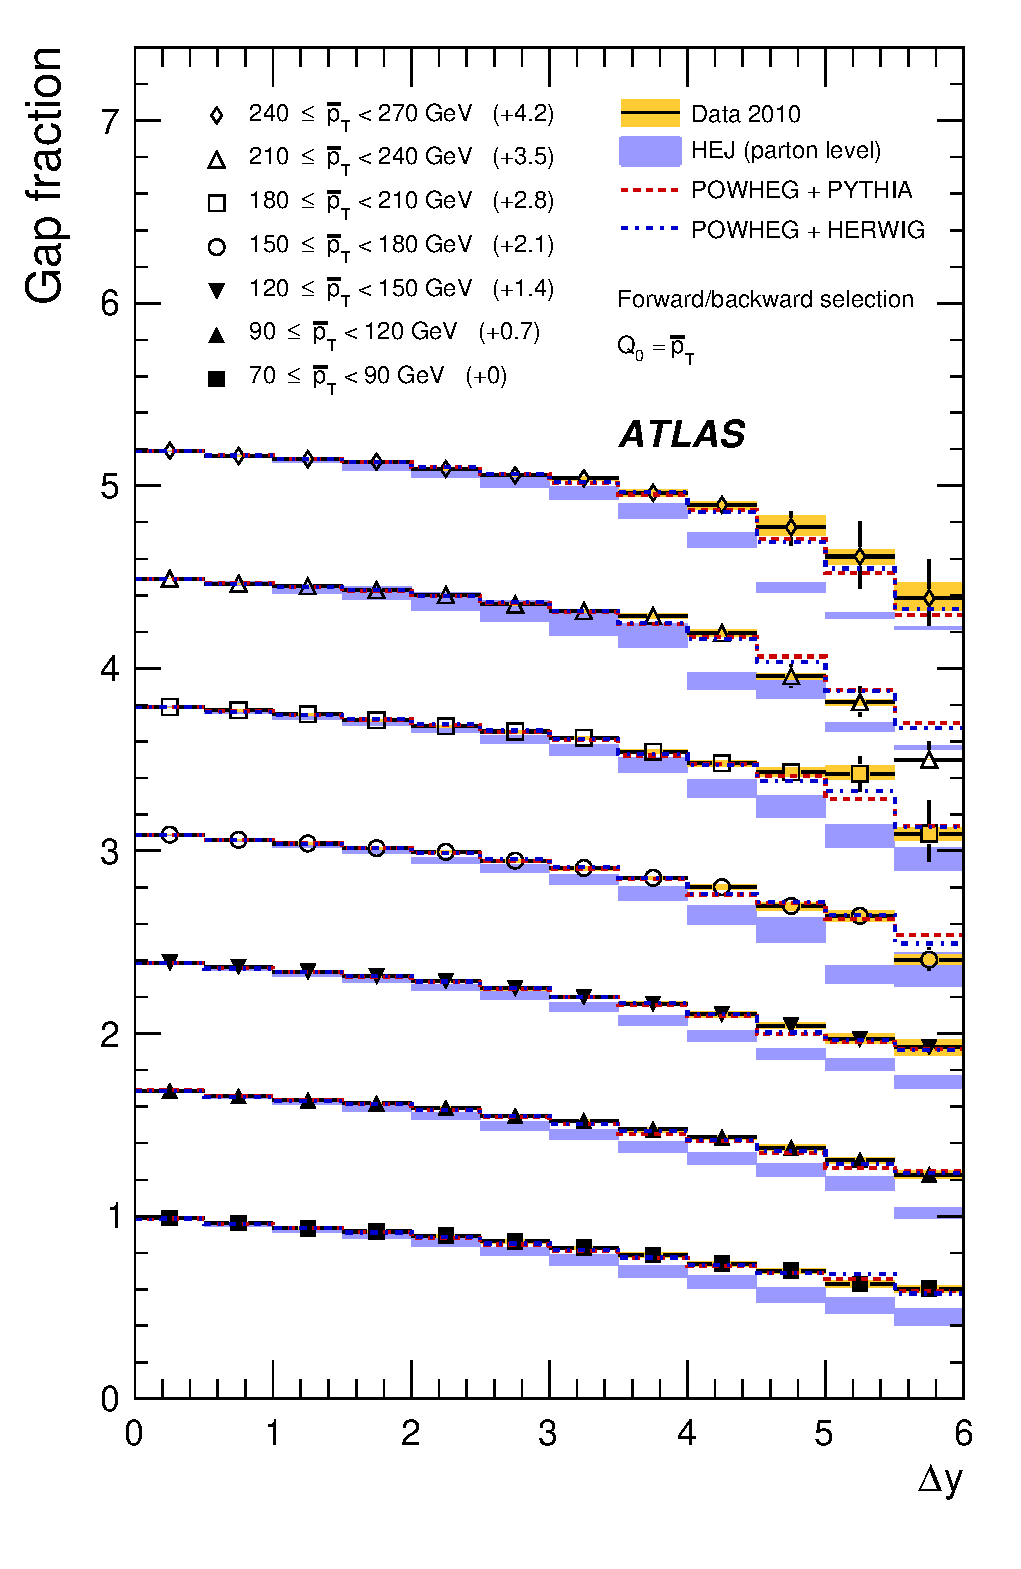
\includegraphics[width=\smallfigwidth]{chapters/gbj/GapFraction_YDist_gap_ptbar_sel_B.eps}
    \label{fig:gbj:Gap_fraction_dY_Bp_comparison}}
  \quad
  \subfloat[Ratio to theory]{
    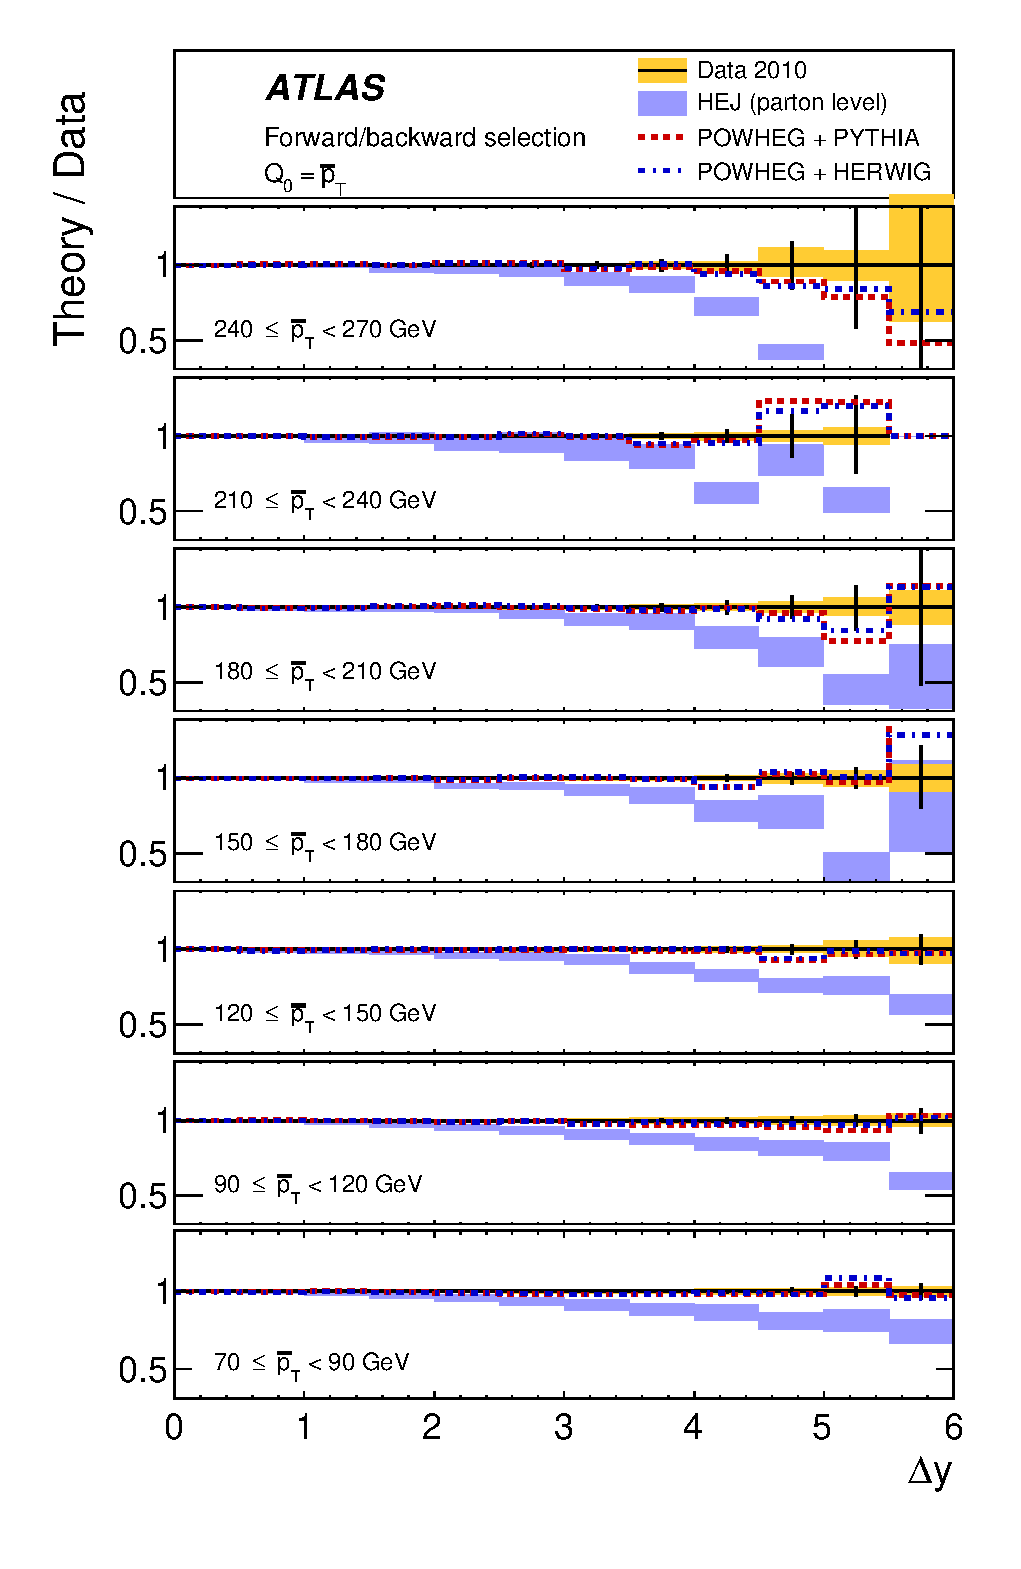
\includegraphics[width=\smallfigwidth]{chapters/gbj/GapFraction_YDist_gap_ptbar_sel_B_Ratio.eps}
    \label{fig:gbj:Gap_fraction_dY_Bp_ratio}}
  \caption{Gap fraction as a function of \DeltaY for seven \pTbar slices, but with
           the veto scale set to $\Qnought = \pTbar$. \protect\subref{fig:gbj:Gap_fraction_dY_Bp_comparison}
           shows selection B data against the \HEJ and \Powheg generators, while \protect\subref{fig:gbj:Gap_fraction_dY_Bp_ratio}
           shows the ratio of the theory predictions to the data. The data and theory
           are presented in the same way as \FigureRef{fig:gbj:Gap_fraction_pTbar_A}.}
  \label{fig:gbj:Gap_fraction_dY_Bp}
\end{figure}

\begin{figure}[htpb]
  \subfloat[\pTbar slices]{
    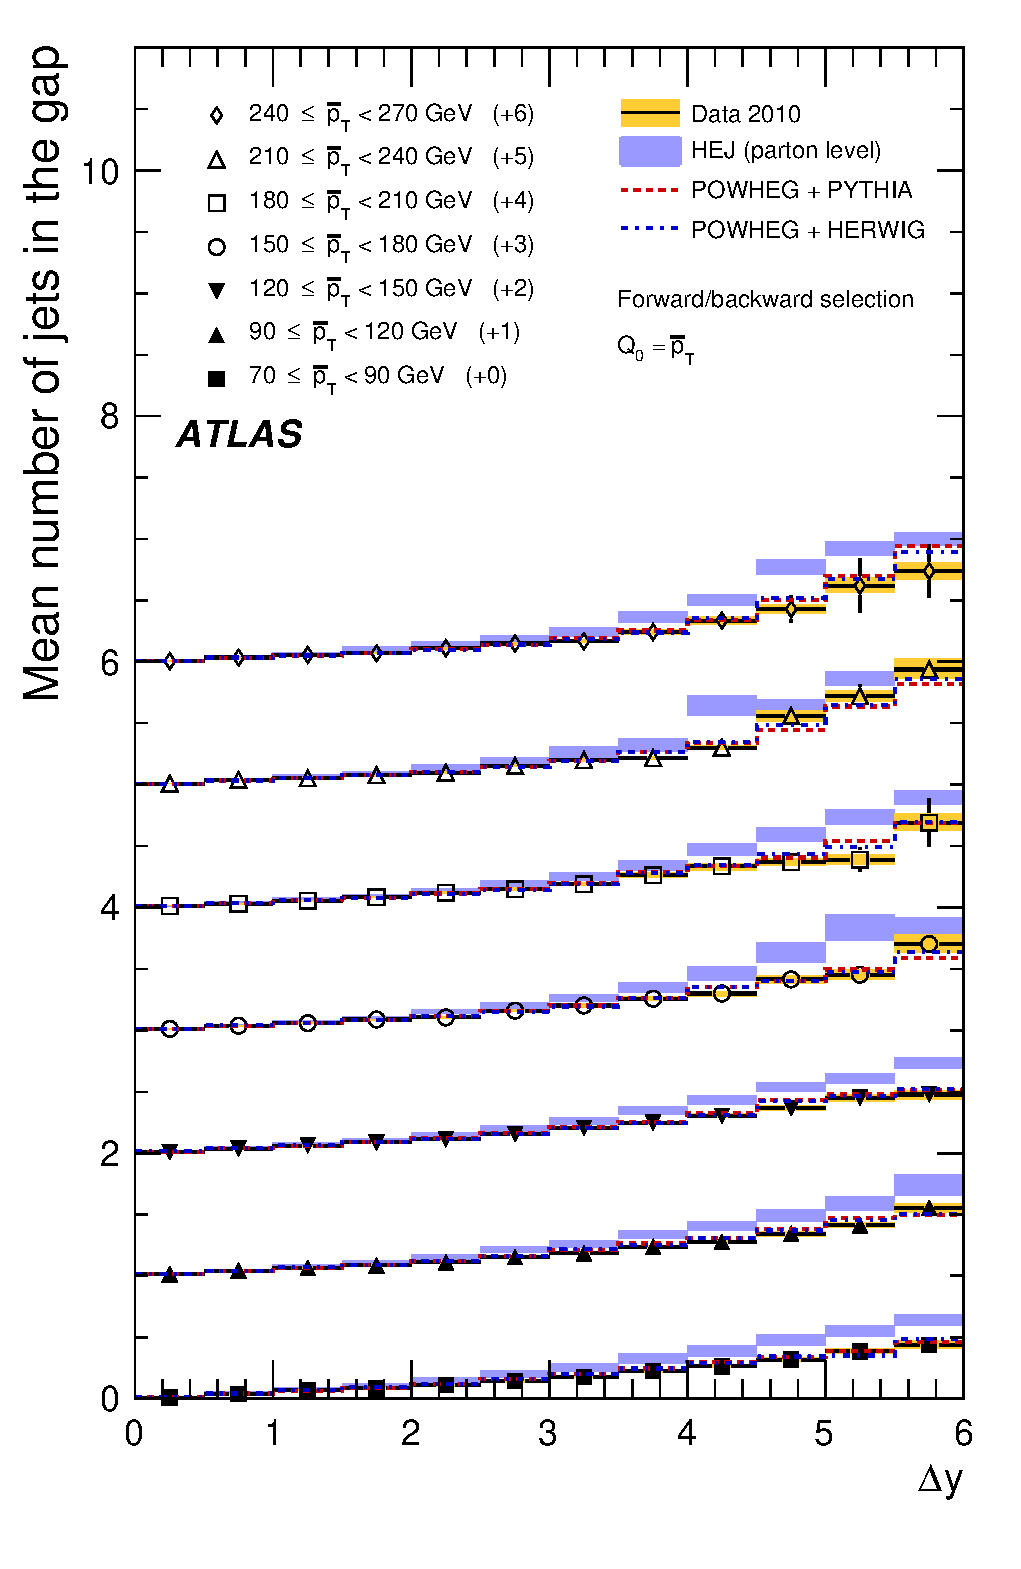
\includegraphics[width=\smallfigwidth]{chapters/gbj/Njet_YDist_gap_ptbar_sel_B.eps}
    \label{fig:gbj:N_jets_dY_Bp_comparison}}
  \quad
  \subfloat[Ratio to theory]{
    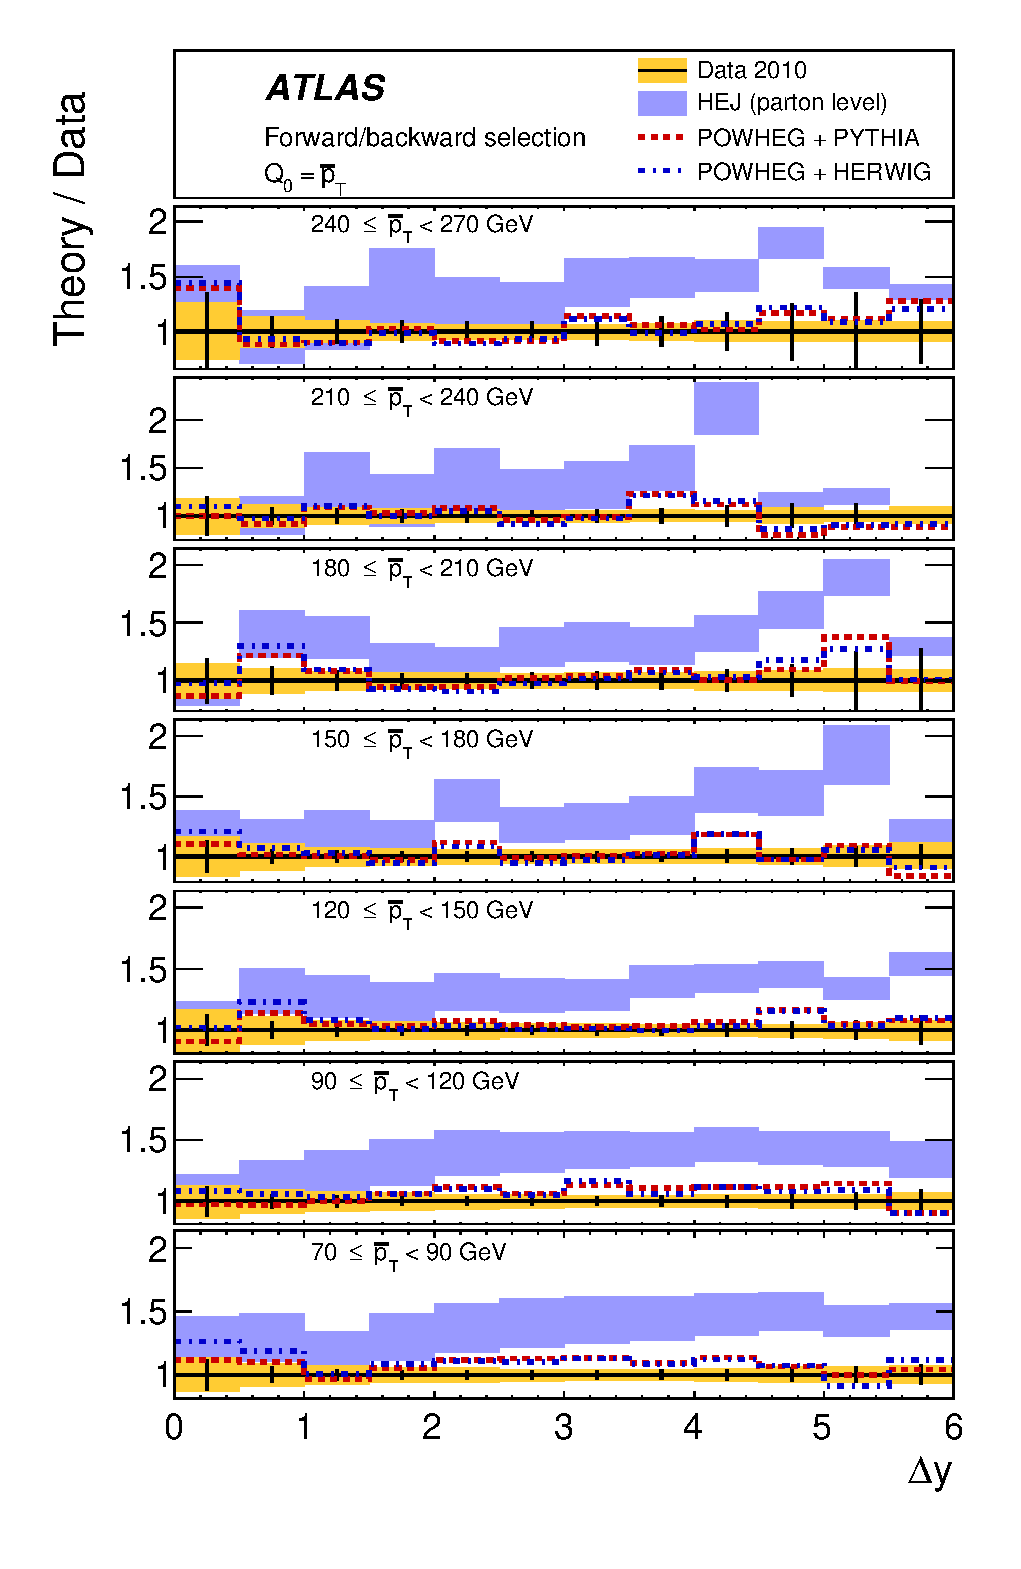
\includegraphics[width=\smallfigwidth]{chapters/gbj/Njet_YDist_gap_ptbar_sel_B_Ratio.eps}
    \label{fig:gbj:N_jets_dY_Bp_ratio}}
  \caption{Mean number of jets in the gap as a function of \DeltaY for seven \pTbar
           slices, but with the veto scale set to $\Qnought = \pTbar$. \protect\subref{fig:gbj:N_jets_dY_Bp_comparison}
           shows selection B data against the \HEJ and \Powheg generators, while \protect\subref{fig:gbj:N_jets_dY_Bp_ratio}
           shows the ratio of the theory predictions to the data. The data and theory
           are presented in the same way as \FigureRef{fig:gbj:Gap_fraction_pTbar_A}.}
  \label{fig:gbj:N_jets_dY_Bp}
\end{figure}

\section{Summary}
These results show the expected behaviour of a reduction of gap events for
harder jets and for larger rapidity gaps~\cite{Forshaw:2009:JetVeto} for both
selections. There are some interesting deviations between the data and the
various theory calculations, in particular, the parton level \HEJ prediction
deviates from the data at large \DeltaY and large $\pTbar / \Qnought$; areas of
phase space in which it was expected that it should perform well. \Powheg generally describes the data well when interfaced to \Pythia,
except at large \DeltaY, and performs much more poorly when combined with \Herwig.

Experimental uncertainties are smaller than the theoretical ones for most of the
phase-space considered here. In addition, the experimental uncertainty is
smaller than the spread of \MC event generator predictions. These results could,
therefore, be used to constrain the modelling of \QCD radiation in widely
separated \dijet systems, leading to an improved understanding of the behaviour
of jet vetoes for future measurements. This work was published in the Journal of
High Energy Physics~\cite{JHEP:2011:ATLAS_GBJ}.
